
\section{Benchmark IS}
Celem eksperymentów była ocena efektywności implementacji algorytmu sortowania całkowitoliczbowego (Integer Sort, IS) w czterech wersjach programistycznych (\texttt{new\_omp}, \texttt{old\_omp}, \texttt{tbb}, \texttt{rust}) przy różnych klasach problemów (S, W, A, B) i liczbie wątków. Porównanie obejmuje czas wykonania, wydajność (MFLOPS) oraz współczynnik zmienności (CV - coefficient of variation), obrazujący stabilność pomiarową.

\subsection{Wyniki benchmarków - platforma ARM64}
\begin{figure}[!h]
    \centering
    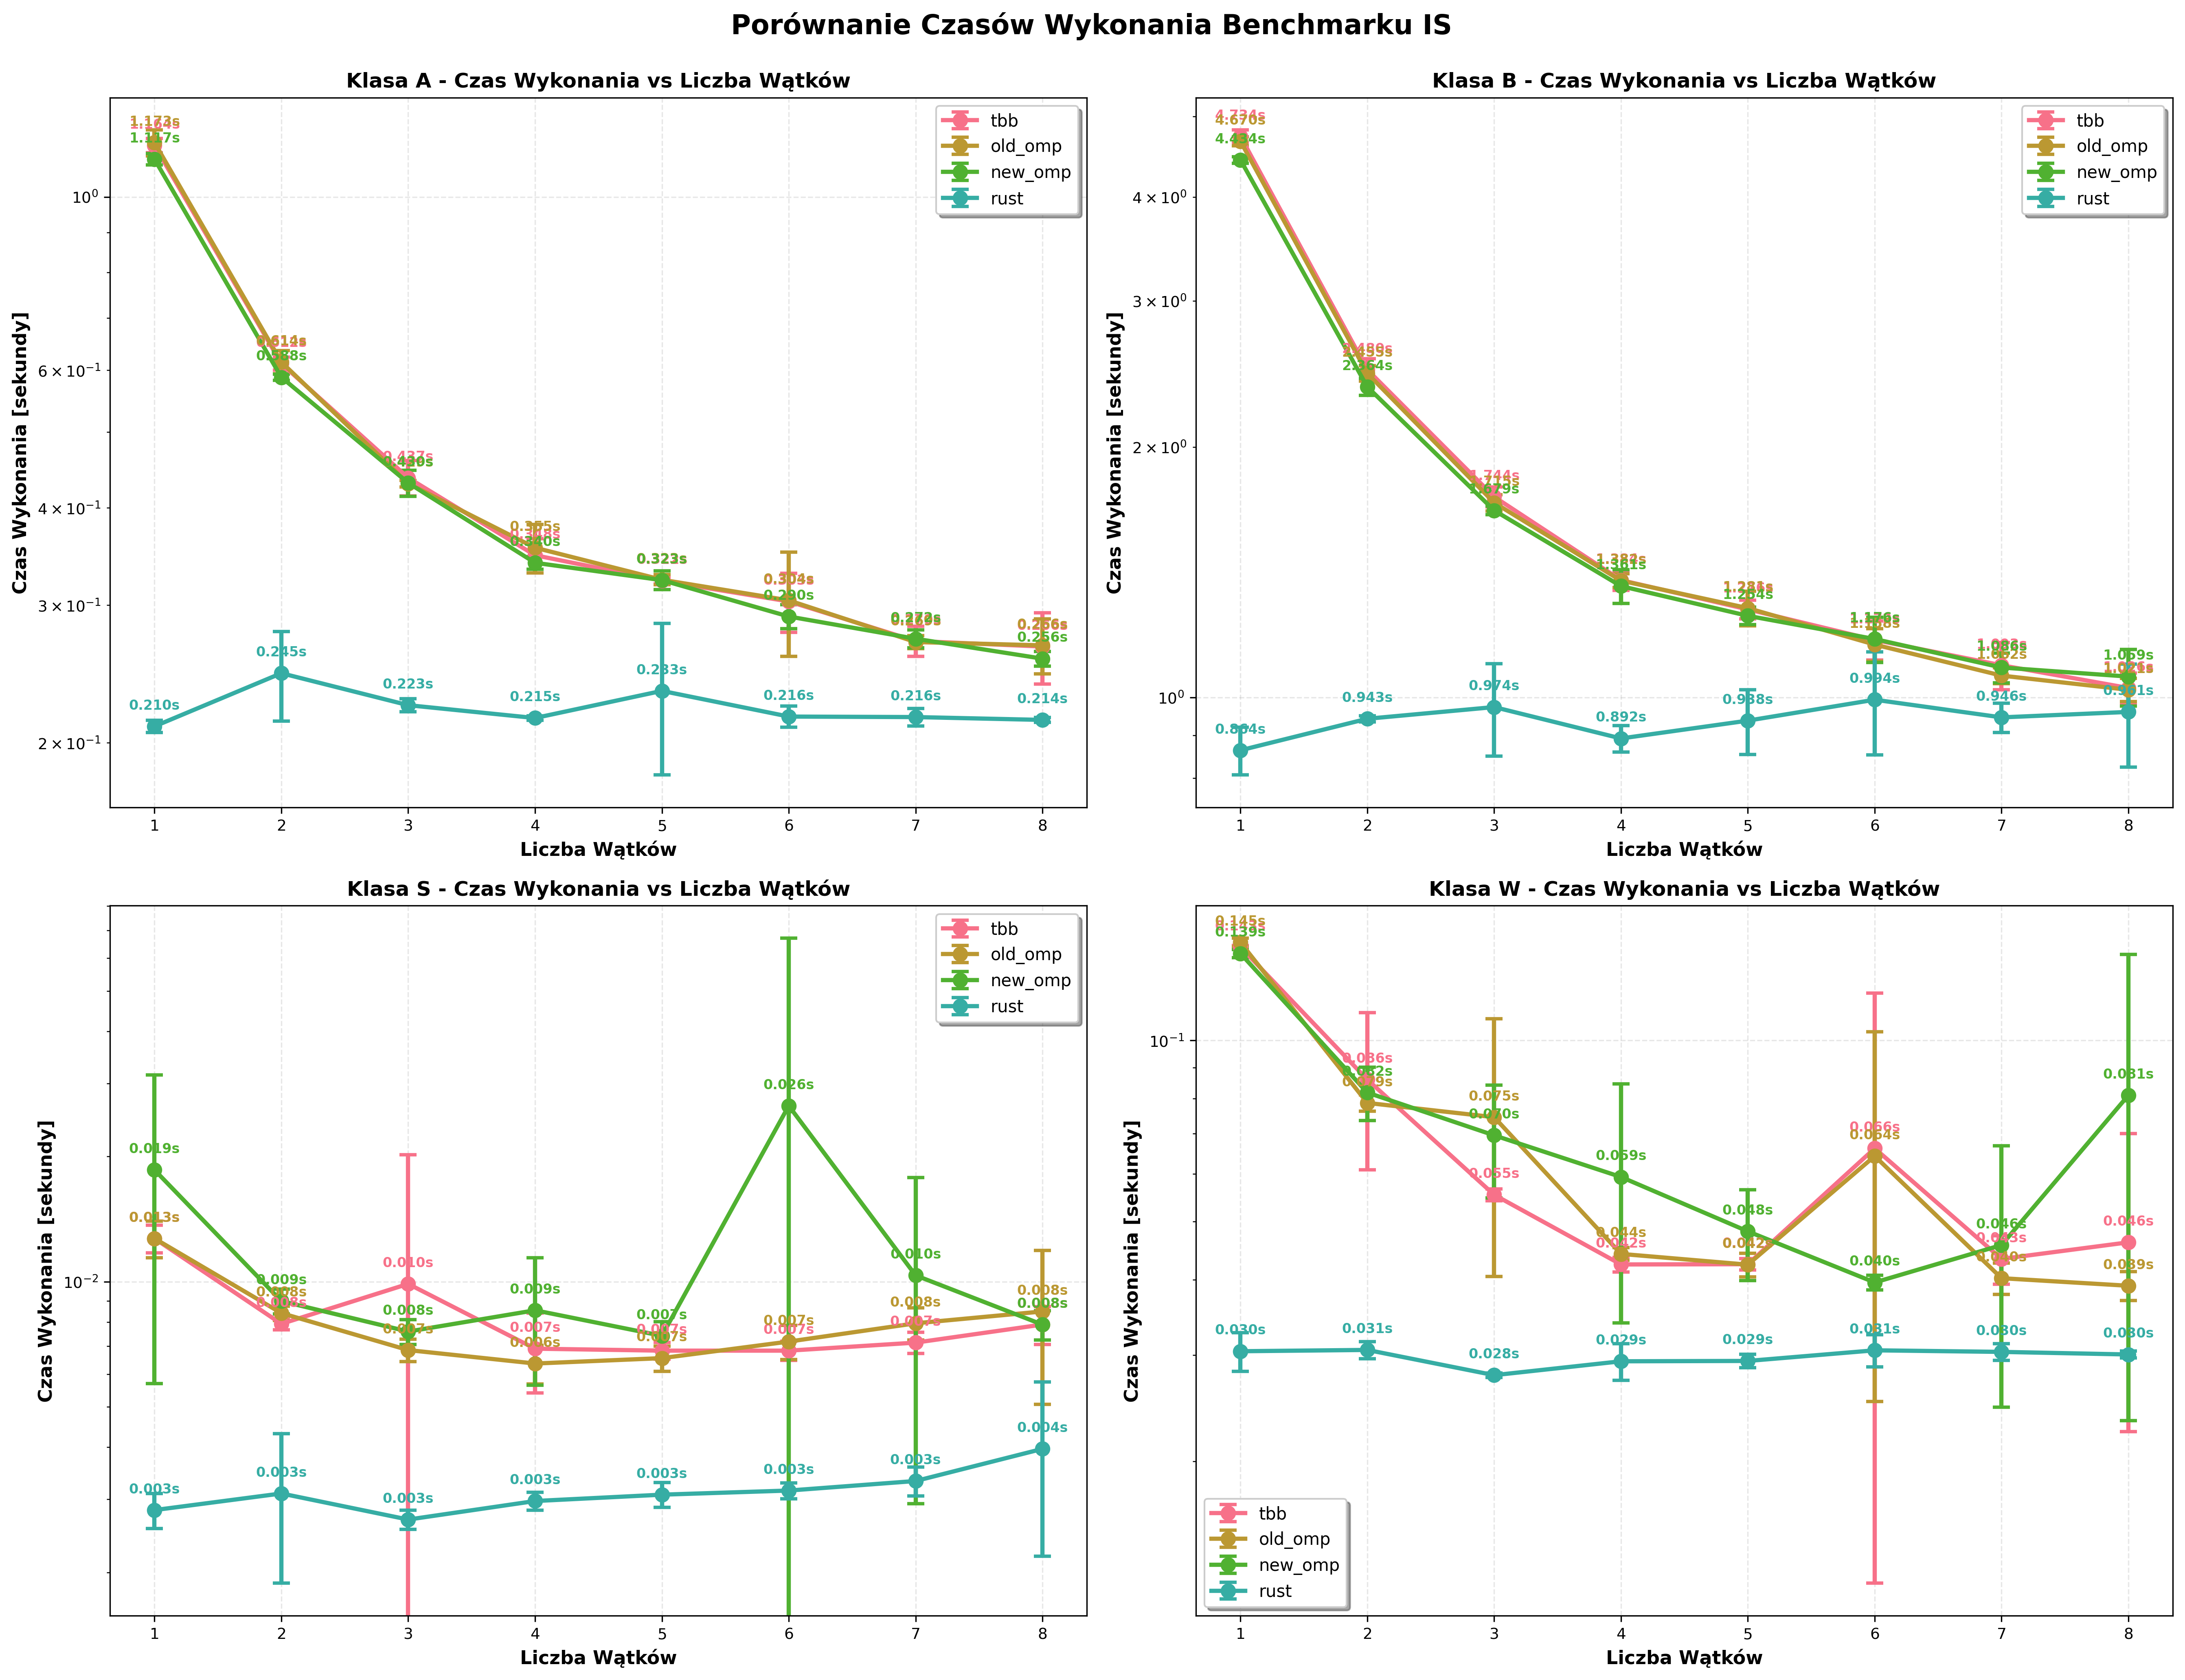
\includegraphics[width=0.9\textwidth]{analiza/images/parallel/is/arm/is_porownanie_czasow_wykonania.png}
    \caption{Porównanie czasów wykonania benchmarku IS dla klas S, W, A, B względem liczby użytych wątków}
    \label{is_porownanie_czasow_wykonania}
\end{figure}

Na wykresie - rysunek \ref{is_porownanie_czasow_wykonania} najbardziej znaczącym obserwowanym zjawiskiem jest dominacja implementacji w języku Rust, która osiąga zdecydowanie najkrótsze czasy wykonania we wszystkich klasach problemu oraz dla wszystkich konfiguracji liczby wątków. W szczególności w klasach A i B różnice pomiędzy Rust a pozostałymi implementacjami są bardzo wyraźne i sięgają nawet kilku razy krótszych czasów wykonania, co sugeruje fundamentalnie bardziej efektywną organizację obliczeń.

W przypadku klas A i B wszystkie implementacje, z wyjątkiem Rust, wykazują systematyczny spadek czasu wykonania wraz ze wzrostem liczby wątków. Na skali logarytmicznej zależność ta przyjmuje niemal liniowy charakter, co oznacza, że wzrost liczby wątków przekłada się na wykładniczą poprawę wydajności. Szczególnie dobrze skalują się implementacje oparte na bibliotekach \texttt{tbb} oraz OpenMP (zarówno \texttt{old\_omp}, jak i \texttt{new\_omp}), co potwierdza skuteczność zastosowanych modeli równoległości dla dużych, dobrze zbalansowanych zadań.

Można zauważyć kolejne odrębne zjawisko dla implementacji w \texttt{rust}, której charakterystyka czasów wykonania przy zwiększaniu liczby wątków pozostaje stosunkowo płaska. Sugeruje to, że implementacja ta osiąga bardzo wysoką wydajność już przy niskim poziomie równoległości, a dalsze zwiększanie liczby wątków nie przynosi istotnych korzyści.

W mniejszych klasach problemu, takich jak S i W, obserwuje się znacznie większą nieregularność skalowania oraz większą wariancję wyników. Jest to zgodne z oczekiwaniami, ponieważ dla niewielkich zadań narzuty związane z uruchamianiem i synchronizacją wątków często przewyższają potencjalne zyski z ich równoległego wykonania. Szczególnie widoczne jest to w~przypadku implementacji \texttt{new\_omp}, która w klasie W wykazuje nawet wzrost czasu wykonania przy 6 i 8 wątkach, co może być efektem niewłaściwego rozkładu pracy lub kosztów synchronizacji przewyższających zyski z równoległości.

Dalsza analiza \ref{is_porownanie_czasow_wykonania} według klas problemu pozwala zauważyć, że w klasach A i B - reprezentujących większe instancje obliczeniowe - implementacje \texttt{\texttt{tbb}}, \texttt{old\_omp} i \texttt{new\_omp} osiągają bardzo podobne czasy wykonania i wykazują zbliżone wzorce skalowania. Ich wydajność rośnie do poziomu 8 wątków, po czym tempo przyrostu stopniowo maleje. W tym samym czasie \texttt{rust} konsekwentnie utrzymuje swoją przewagę, osiągając czasy wykonania nawet pięciokrotnie krótsze. W mniejszych klasach (S i W) efektywność równoległości staje się mniej przewidywalna. Różnice między implementacjami są mniej wyraźne, a korzyści z równoległości często stają się marginalne powyżej czterech wątków.

\begin{figure}[H]
    \centering
    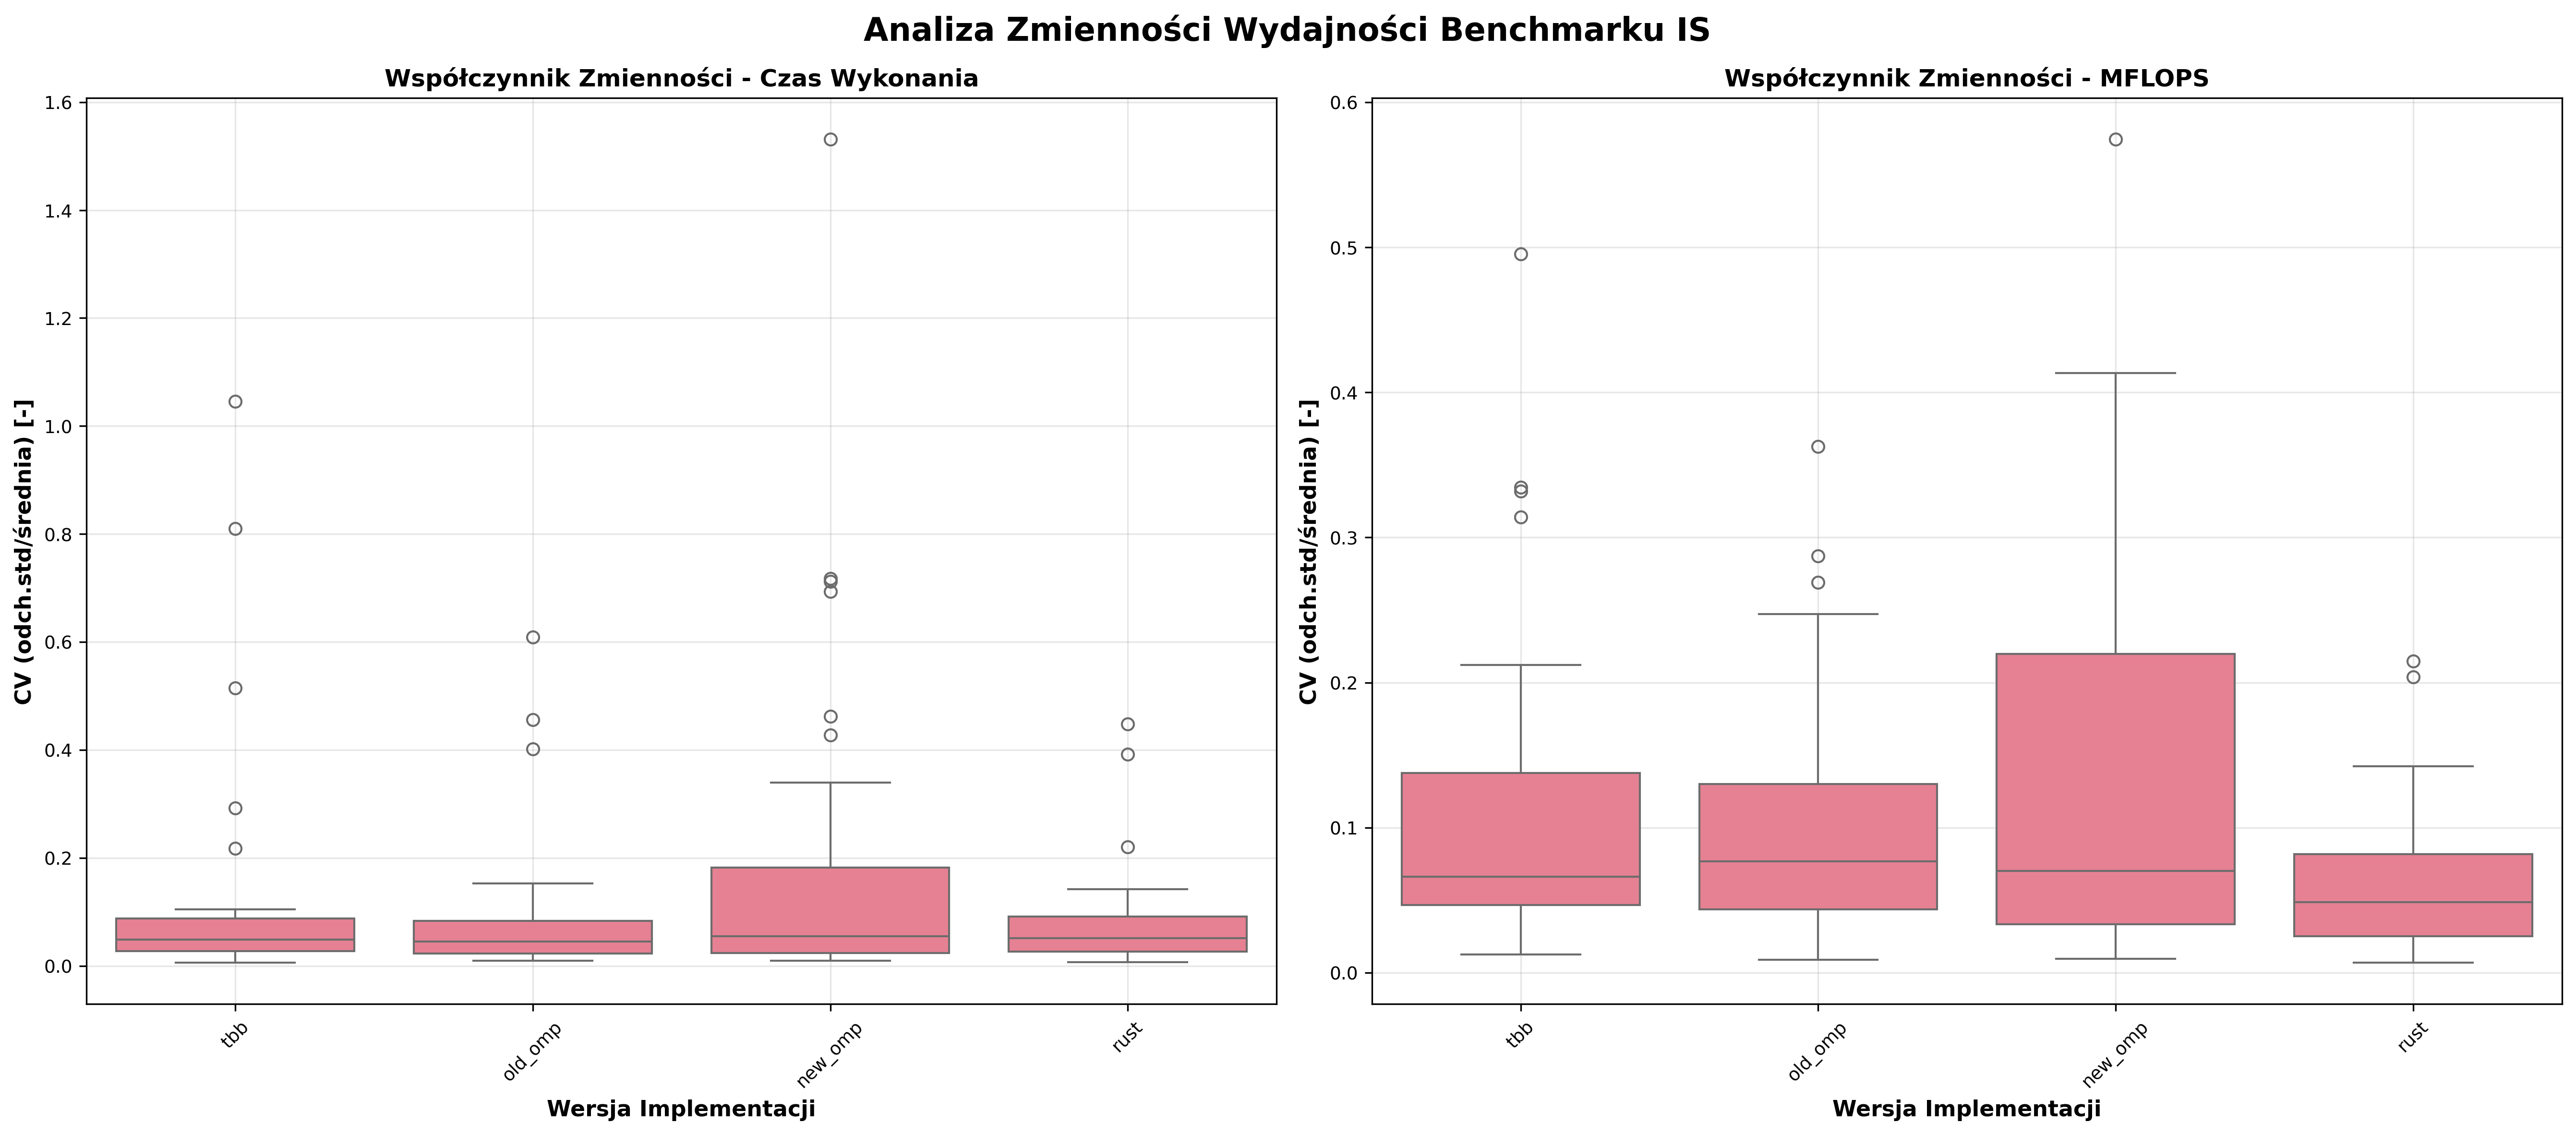
\includegraphics[width=0.9\textwidth]{analiza/images/parallel/is/arm/is_analiza_zmiennosci.png}
    \caption{Analiza zmienności czasów wykonania benchmarku IS dla klas S, W, A, B względem liczby użytych wątków}
    \label{is_analiza_zmiennosci}
\end{figure}

\subsubsection{Analiza zmienności czasu wykonania}
Lewy wykres - rysunek \ref{is_analiza_zmiennosci} ilustruje współczynnik zmienności (CV) dla czasu wykonania. Na jego podstawie można zauważyć, że większość pomiarów, niezależnie od użytej implementacji, cechuje się niskim poziomem zmienności - wartości median CV mieszczą się w zakresie od około 0,05 do 0,1. Świadczy to o wysokiej powtarzalności wyników i braku istotnych fluktuacji czasowych w typowych warunkach testowych.

Spośród wszystkich badanych rozwiązań, implementacja napisana w języku Rust charakteryzuje się najniższą medianą współczynnika zmienności, co wskazuje na najbardziej przewidywalne czasy wykonania. Z kolei implementacja \texttt{new\_omp} wykazuje nieco wyższą zmienność i szerszy rozrzut wartości, co może świadczyć o mniej stabilnym zachowaniu w czasie - być może z powodu większego wpływu czynników systemowych lub charakterystyki zastosowanego modelu równoległości. Warto również zwrócić uwagę na obecność wartości odstających we wszystkich implementacjach. Największe ekstremalne wartości współczynnika zmienności czasu wykonania zaobserwowano w przypadku implementacji \texttt{new\_omp} (sięgające nawet 1,5) oraz \texttt{tbb} (do około 1,05), co może oznaczać sporadyczne przypadki znaczącej niestabilności czasowej.

\subsubsection{Analiza zmienności MFLOPS}
Drugi wykres przedstawia zmienność metryki MFLOPS, która - mimo że pochodna względem czasu wykonania - wykazuje ogólnie wyższy poziom zmienności. Jest to zrozumiałe, biorąc pod uwagę, że wskaźnik ten jest bardziej podatny na mikrofluktuacje w wydajności procesora, zarządzanie energią czy zmiany częstotliwości taktowania. Również tutaj implementacja \texttt{new\_omp} wyróżnia się najwyższą medianą współczynnika zmienności oraz największym rozrzutem wartości, co potwierdza jej ograniczoną stabilność pod względem uzyskiwanej wydajności. Z drugiej strony, implementacja Rust ponownie osiąga najlepsze wyniki, z najniższą zmiennością i~relatywnie wąskim zakresem obserwowanych wartości, co świadczy o jej konsekwentnej wydajności niezależnie od liczby powtórzeń czy konfiguracji.

Rozkład współczynnika zmienności MFLOPS jest ogólnie mniej symetryczny niż w przypadku czasu wykonania. Szczególnie dla implementacji \texttt{tbb} i \texttt{new\_omp} obserwuje się wyraźną asymetrię wykresów pudełkowych, co może sugerować występowanie bardziej złożonych zjawisk wpływających na wahania wydajności. Najwyższa wartość odstająca w tym przypadku - około 0,58 - również dotyczy implementacji \texttt{new\_omp}, co po raz kolejny podkreśla jej względnie niższą stabilność. Ogółem, analiza zmienności wskazuje, że choć większość implementacji zapewnia akceptowalny poziom powtarzalności, to Rust wyróżnia się nie tylko pod względem szybkości, ale również przewidywalności działania, co czyni go najbardziej stabilnym rozwiązaniem spośród badanych.
%------------------------------
\begin{figure}[H]
    \centering
    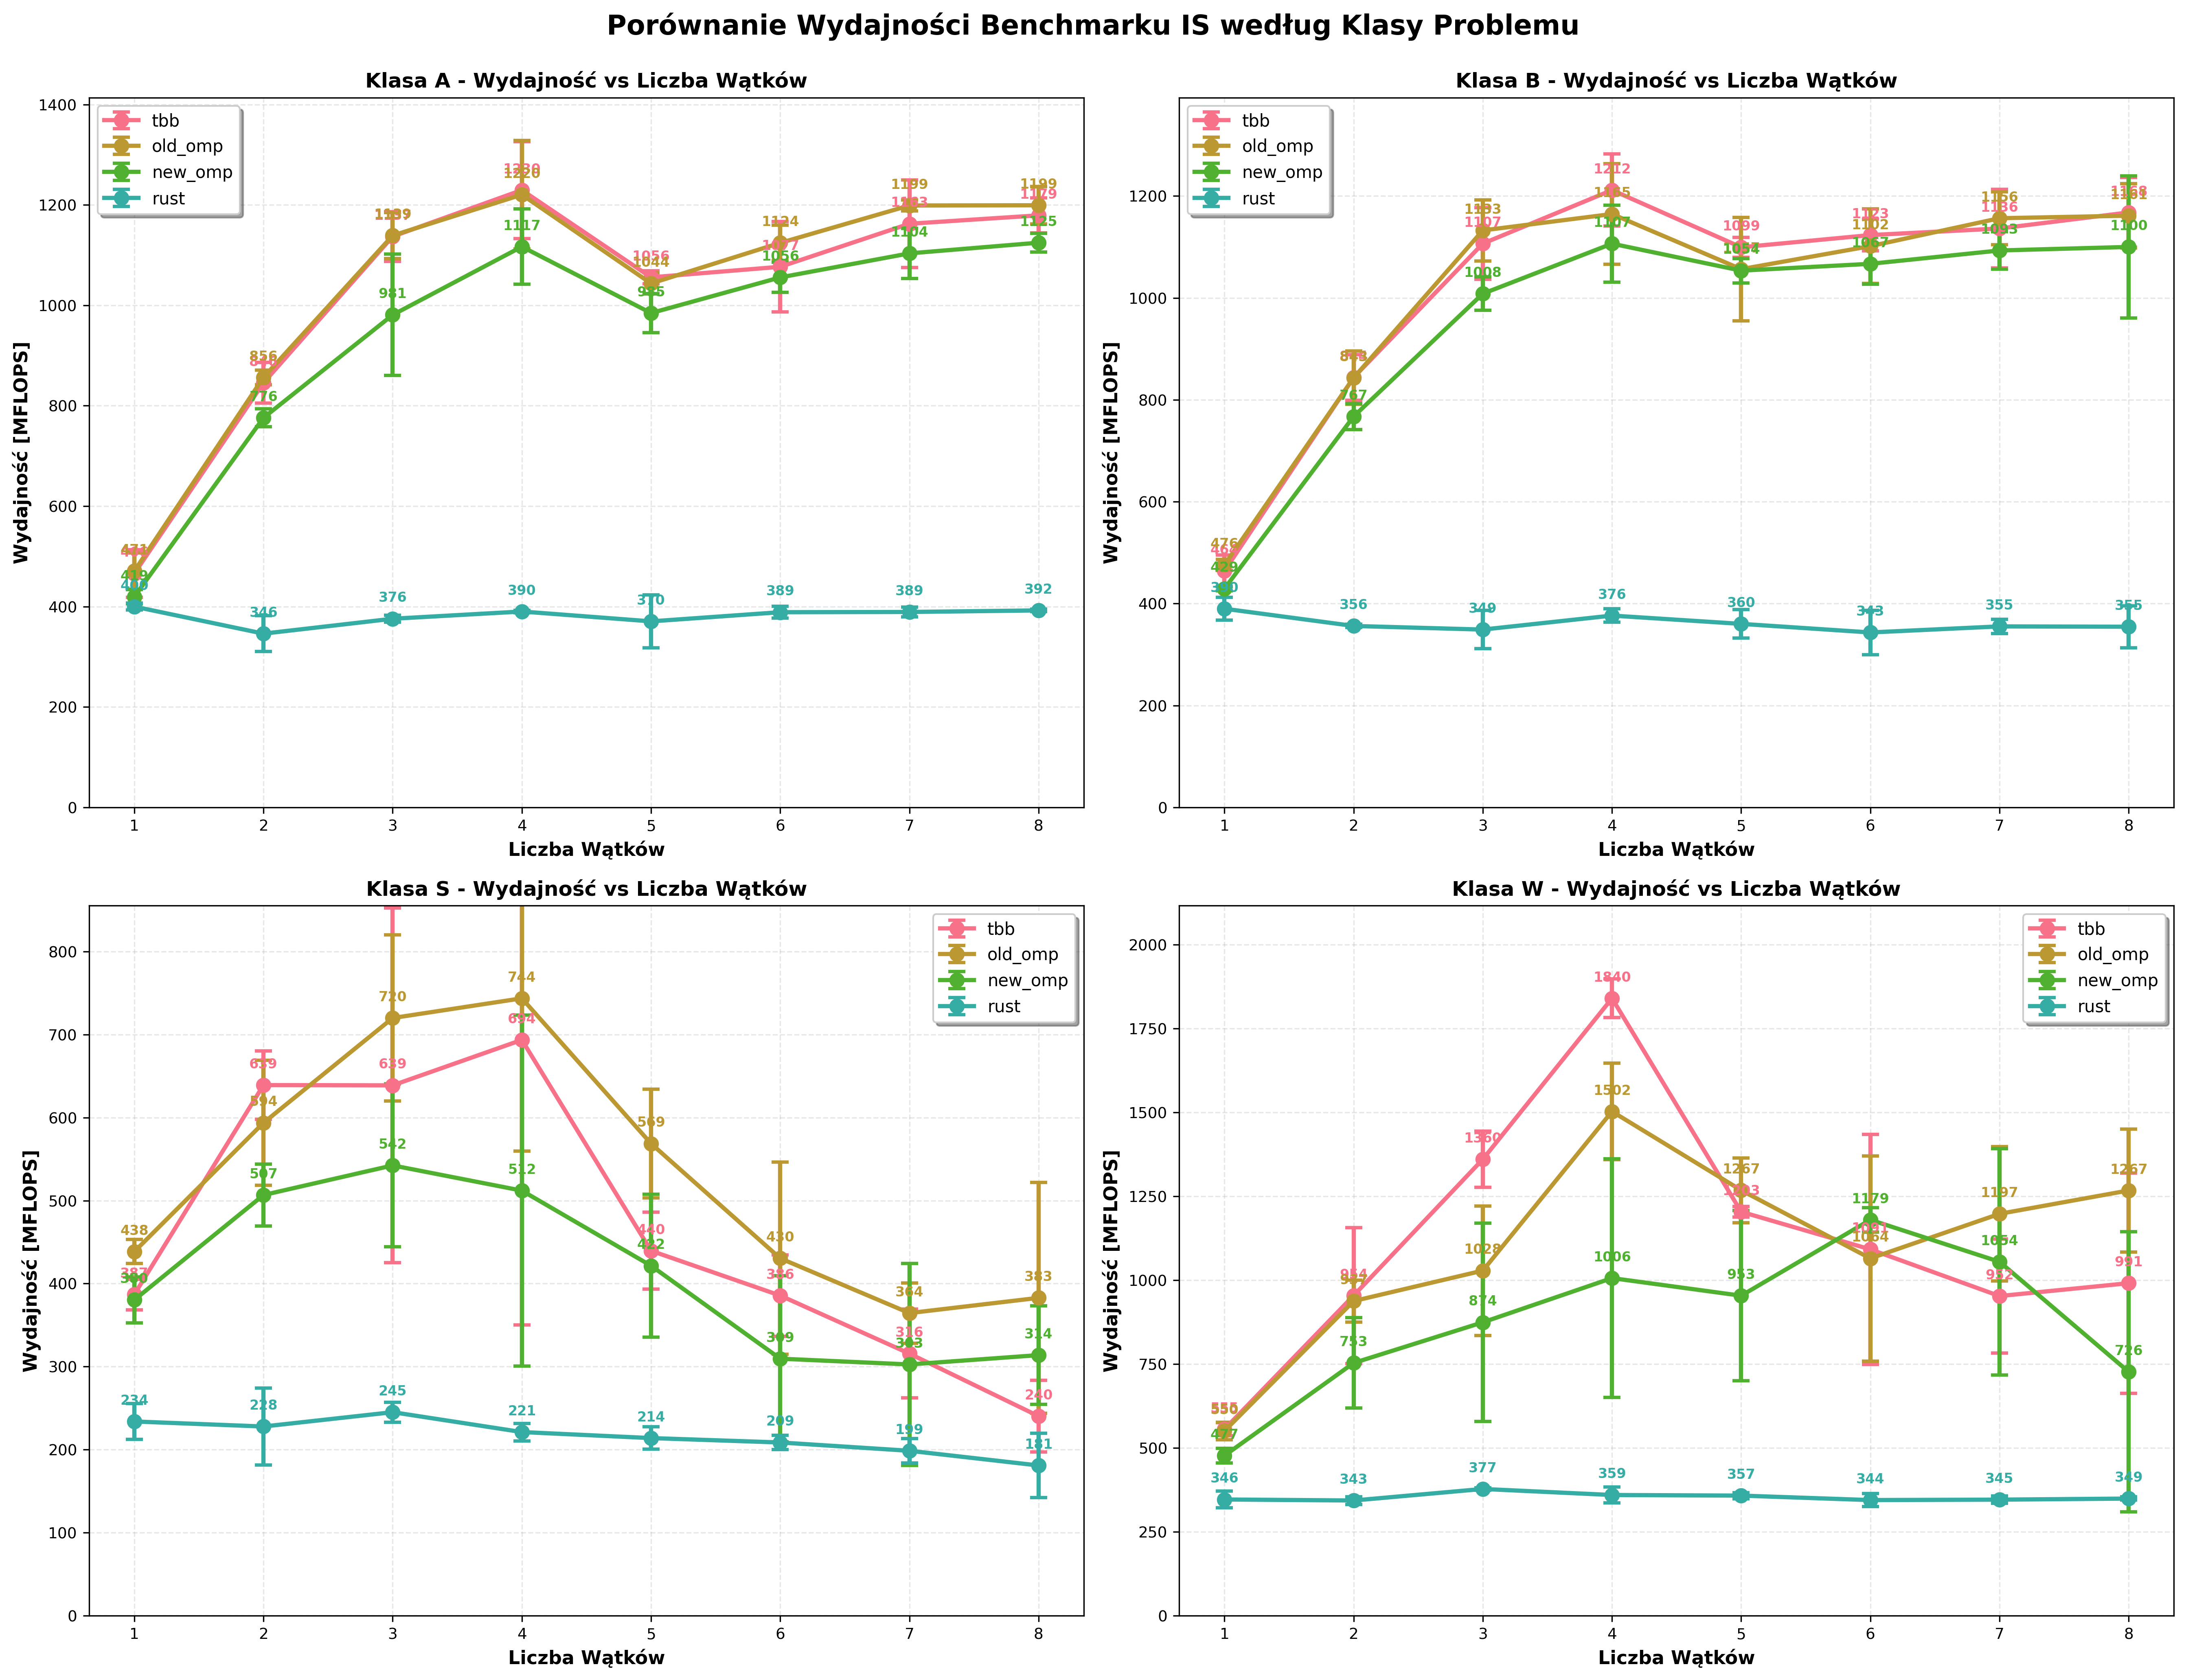
\includegraphics[width=0.9\textwidth]{analiza/images/parallel/is/arm/is_porownanie_wydajnosci.png}
    \caption{Porównanie wydajności benchmarku IS dla klas S, W, A, B względem liczby użytych wątków}
    \label{is_porownanie_wydajnosci}
\end{figure}
Na wykresach na rysunku \ref{is_porownanie_wydajnosci} zaprezentowano porównanie wydajności benchmarku IS mierzonej w MFLOPS (milionach operacji zmiennoprzecinkowych na sekundę). Wydajność została przedstawiona jako funkcja liczby wątków (1-8) dla czterech implementacji równoległych.

Analiza zależności wydajności od liczby wątków ujawnia nietypowy wzorzec skalowania. W przeciwieństwie do klasycznych benchmarków, w których można zaobserwować proporcjonalny wzrost wydajności wraz ze wzrostem liczby wątków, implementacje \texttt{tbb}, \texttt{old\_omp} oraz \texttt{new\_omp} wykazują poprawę wydajności jedynie do poziomu 3-4 wątków. Po tym punkcie wydajność zaczyna się stabilizować, a w niektórych przypadkach wręcz nieznacznie spada. Może to wskazywać na istnienie fundamentalnych ograniczeń wynikających z przepustowości pamięci lub narzutu synchronizacji, które skutecznie ograniczają dalsze korzyści wynikające z równoległości.

W przypadku mniejszych klas problemowych, takich jak S i W, obserwowane wzorce są jeszcze bardziej nieregularne. Wydajność często osiąga maksimum przy 3-4 wątkach, po czym wyraźnie spada. Szczególnie interesujący jest przypadek implementacji \texttt{tbb} w klasie W, która osiąga imponującą wartość 1840 MFLOPS przy czterech wątkach - najwyższą ze wszystkich konfiguracji w całym badaniu. Takie lokalne maksima sugerują silną zależność algorytmu od konkretnej wielkości danych i liczby wątków, co może wynikać z efektów dopasowania do rozmiaru cache lub harmonogramu zadań.

W wyraźnym kontraście pozostaje implementacja w języku Rust, która wykazuje niezwykle stabilne zachowanie. Jej wydajność pozostaje na stosunkowo stałym poziomie bez względu na liczbę wątków. Choć osiągane wartości MFLOPS są zauważalnie niższe niż w pozostałych implementacjach - dla klas A i B mieszczą się w zakresie 350-400 MFLOPS, a dla S i W wynoszą 200-350 MFLOPS - to cechują się wysoką regularnością. Taki rozkład sugeruje, że Rust wykorzystuje inną strategię wykonania, bardziej odporną na zmienność środowiska wykonawczego, ale jednocześnie mniej efektywną w pełnym wykorzystaniu potencjału równoległego sprzętu.

Porównując osiągi różnych implementacji, zauważa się wyraźną dominację \texttt{tbb} i \texttt{old\_omp} w klasach A i B. Obie te implementacje osiągają szczytowe wartości na poziomie około \mbox{1200 MFLOPS} przy użyciu 3-4 wątków, natomiast \texttt{new\_omp} nieznacznie ustępuje im, osiągając maksymalnie około 1100 MFLOPS. Różnice te są niewielkie, ale powtarzalne i mogą wskazywać na subtelne różnice w sposobie zarządzania wątkami lub rozdzielania zadań.

W mniejszych klasach problemowych różnice pomiędzy implementacjami są wyraźniejsze, a~uzyskane rezultaty mniej przewidywalne. Po raz kolejny wyróżnia się tutaj implementacja \texttt{tbb}, która w klasie W bije rekord wydajności, osiągając wspomniane 1840 MFLOPS. Skalowanie w tych klasach jest nierówne i często nieliniowe, co świadczy o dużej wrażliwości na liczbę wątków oraz właściwości algorytmu w kontekście niewielkich zbiorów danych.

Implementacja \texttt{rust} utrzymuje konsekwentnie niższy poziom wydajności we wszystkich klasach i konfiguracjach. Jest to zaskakujące, biorąc pod uwagę jej bardzo dobre wyniki w innych benchmarkach, takich jak EP.
\begin{figure}[H]
    \centering
    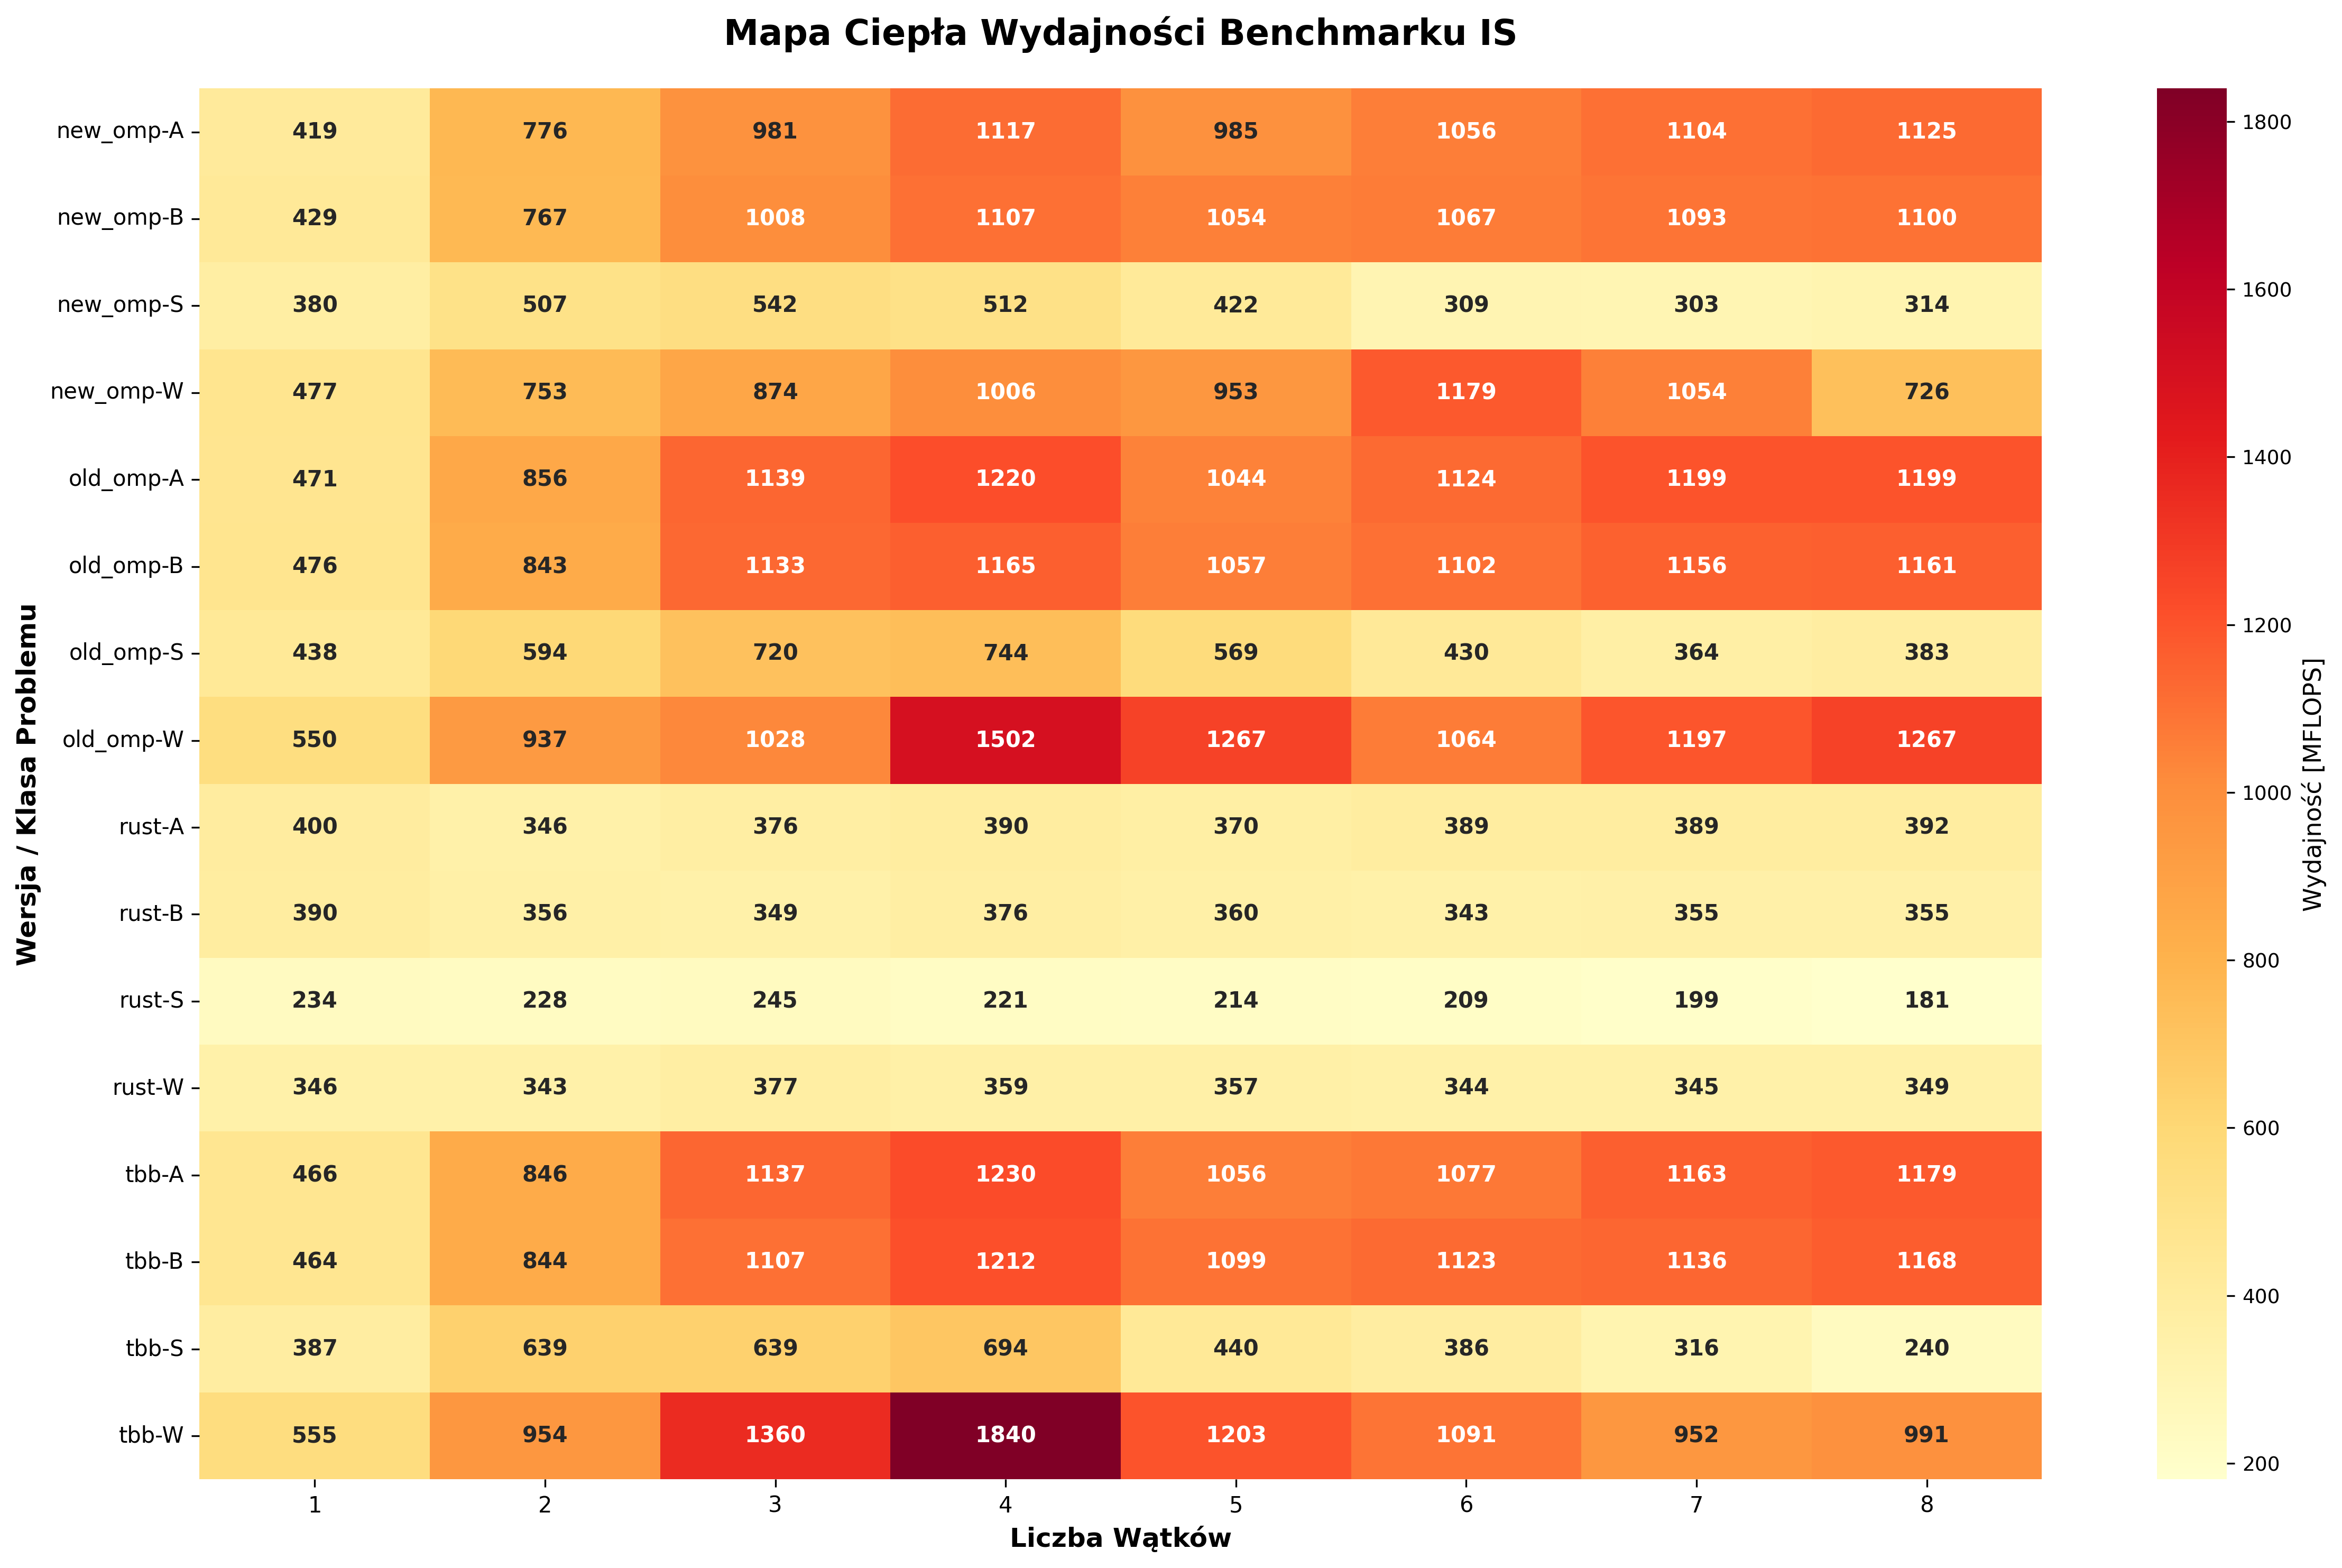
\includegraphics[width=0.9\textwidth]{analiza/images/parallel/is/arm/is_mapa_ciepla_wydajnosci.png}
    \caption{Mapa ciepła wydajności benchmarku IS dla klas S, W, A, B względem liczby użytych wątków}
    \label{is_heatmap_wydajnosci}
\end{figure}
Powyższa mapa cieplna - rysunek \ref{is_heatmap_wydajnosci} przedstawia wydajność (w MFLOPS). Wydajność została przedstawiona w zależności od liczby użytych wątków. Odcienie koloru od żółtego do ciemnoczerwonego wskazują na wzrost wydajności.

W klasie S wydajność wszystkich implementacji jest wyraźnie niższa, co manifestuje się jako jaśniejszy poziomy pas na mapie. Jest to efekt słabego skalowania oraz niewielkich rozmiarów danych, które ograniczają możliwość efektywnego podziału pracy między wątki. Z kolei wiersze odpowiadające implementacji \texttt{rust} są dość jednolite i jasne, co potwierdza zarówno niższą ogólną wydajność, jak i brak znaczącego wpływu liczby wątków na wynik końcowy.

Wreszcie, klasa W ukazuje największe wahania, co dobrze ilustrują nieregularne "gorące punkty” - obszary lokalnej maksymalnej wydajności wśród ogólnego spadku, szczególnie dla \texttt{tbb} i \texttt{old\_omp}. Te wahania wskazują na wysoką czułość algorytmu IS względem parametrów wykonania i potwierdzają, że efektywność obliczeń w tym benchmarku jest silnie uzależniona od konkretnych kombinacji danych wejściowych i zasobów sprzętowych

\begin{figure}[H]
    \centering
    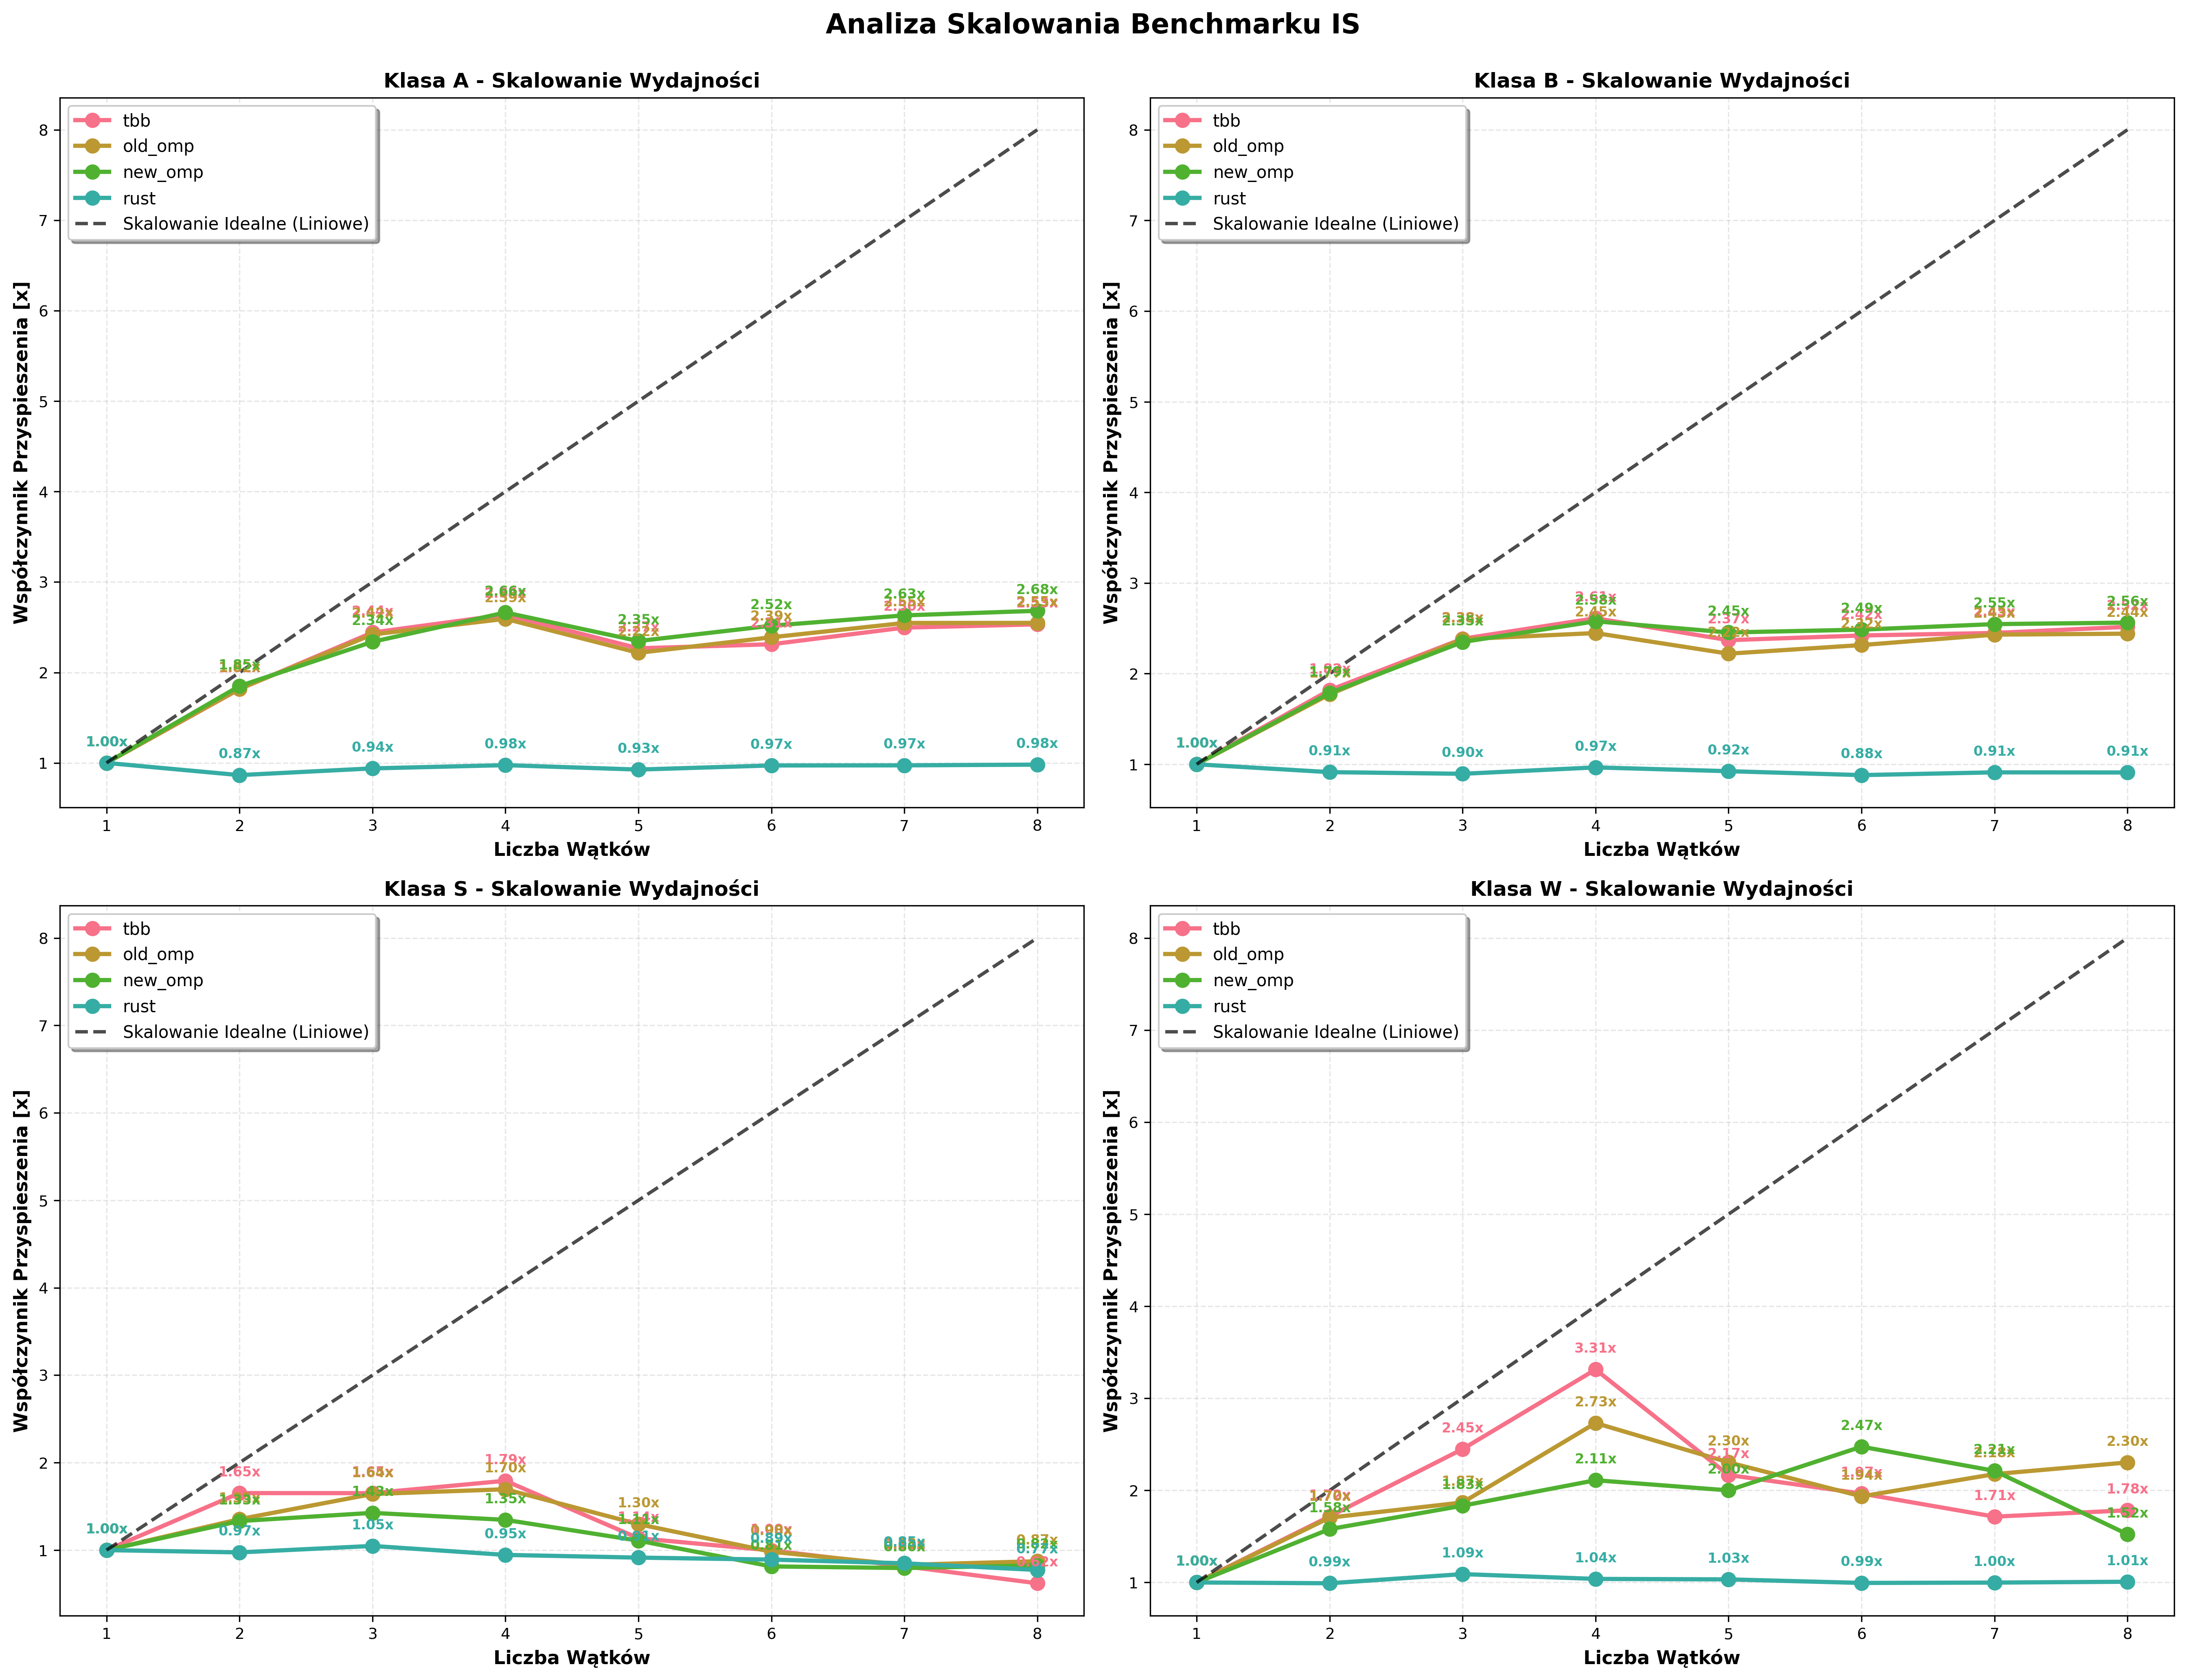
\includegraphics[width=0.9\textwidth]{analiza/images/parallel/is/arm/is_analiza_skalowania.png}
    \caption{Analiza skalowania benchmarku IS dla klas S, W, A, B względem liczby użytych wątków}
    \label{is_analiza_skalowania}
\end{figure}

Analiza wykresów \ref{is_analiza_skalowania} przedstawiających współczynnik przyspieszenia w zależności od liczby wątków ujawnia wyraźne odstępstwa od idealnego skalowania. Choć teoretycznie przyspieszenie powinno rosnąć proporcjonalnie do liczby wątków (co ilustruje linia przerywana na wykresach), w rzeczywistości wartości te osiągają jedynie poziom 2,6-3,3x nawet przy ośmiu wątkach. Taki wynik świadczy o istotnych ograniczeniach efektywności równoległego przetwarzania w przypadku benchmarku IS.

We wszystkich implementacjach i klasach problemowych wyraźnie zaznacza się punkt nasycenia wydajności - lokalna efektywność równoległa osiągana jest zazwyczaj przy 3-4 wątkach. Po przekroczeniu tego progu przyrosty wydajności ulegają zahamowaniu, a w niektórych przypadkach nawet dochodzi do jej spadku. Sugeruje to, że kluczowym czynnikiem ograniczającym skalowanie nie jest sama liczba dostępnych rdzeni, lecz raczej ograniczenia przepustowości pamięci, które uniemożliwiają dalsze równoległe przetwarzanie bez utraty efektywności.

Wielu konfiguracjom towarzyszy również zjawisko niemonotoniczności przyspieszenia. Charakterystyczne są lokalne spadki współczynnika przyspieszenia przy przejściu z 4 do 5 wątków, po czym obserwuje się niewielki wzrost w zakresie 6-8 wątków. Taki przebieg może wskazywać na złożone interakcje między charakterem dostępu do pamięci a architekturą hierarchii cache procesora, które wpływają negatywnie na spójność i przewidywalność skalowania.

Porównując poszczególne implementacje, można zauważyć duże podobieństwo między \texttt{tbb}, \texttt{old\_omp} i \texttt{new\_omp}, szczególnie w klasach problemowych A i B. Wszystkie trzy osiągają maksymalne współczynniki przyspieszenia na poziomie 2,5-2,7x, co sugeruje, że ograniczenia skalowania wynikają przede wszystkim z charakterystyki algorytmu sortowania całkowitoliczbowego IS, a nie z różnic pomiędzy samymi bibliotekami równoległymi.

Na tym tle wyraźnie wyróżnia się implementacja \texttt{tbb} w klasie W, która przy czterech wątkach osiąga współczynnik przyspieszenia wynoszący 3,31x.

Z kolei implementacja napisana w języku Rust prezentuje zupełnie odmienny obraz. Współczynniki przyspieszenia we wszystkich klasach problemowych oscylują wokół wartości 1,0, co oznacza, że praktycznie nie uzyskuje się żadnych korzyści z wykorzystania wielu wątków. Wskazuje to na fundamentalne różnice w implementacji algorytmu lub architekturze mechanizmów współbieżności, które mogą uniemożliwiać efektywne rozproszenie obciążenia obliczeniowego. W rezultacie, mimo znanej stabilności i bezpieczeństwa języka Rust, w tym konkretnym scenariuszu nie udaje się wykorzystać jego potencjału do osiągnięcia przyspieszenia równoległego.

\subsection{Wyniki benchmarków - platforma x86\_64}
\begin{figure}[H]
    \centering
    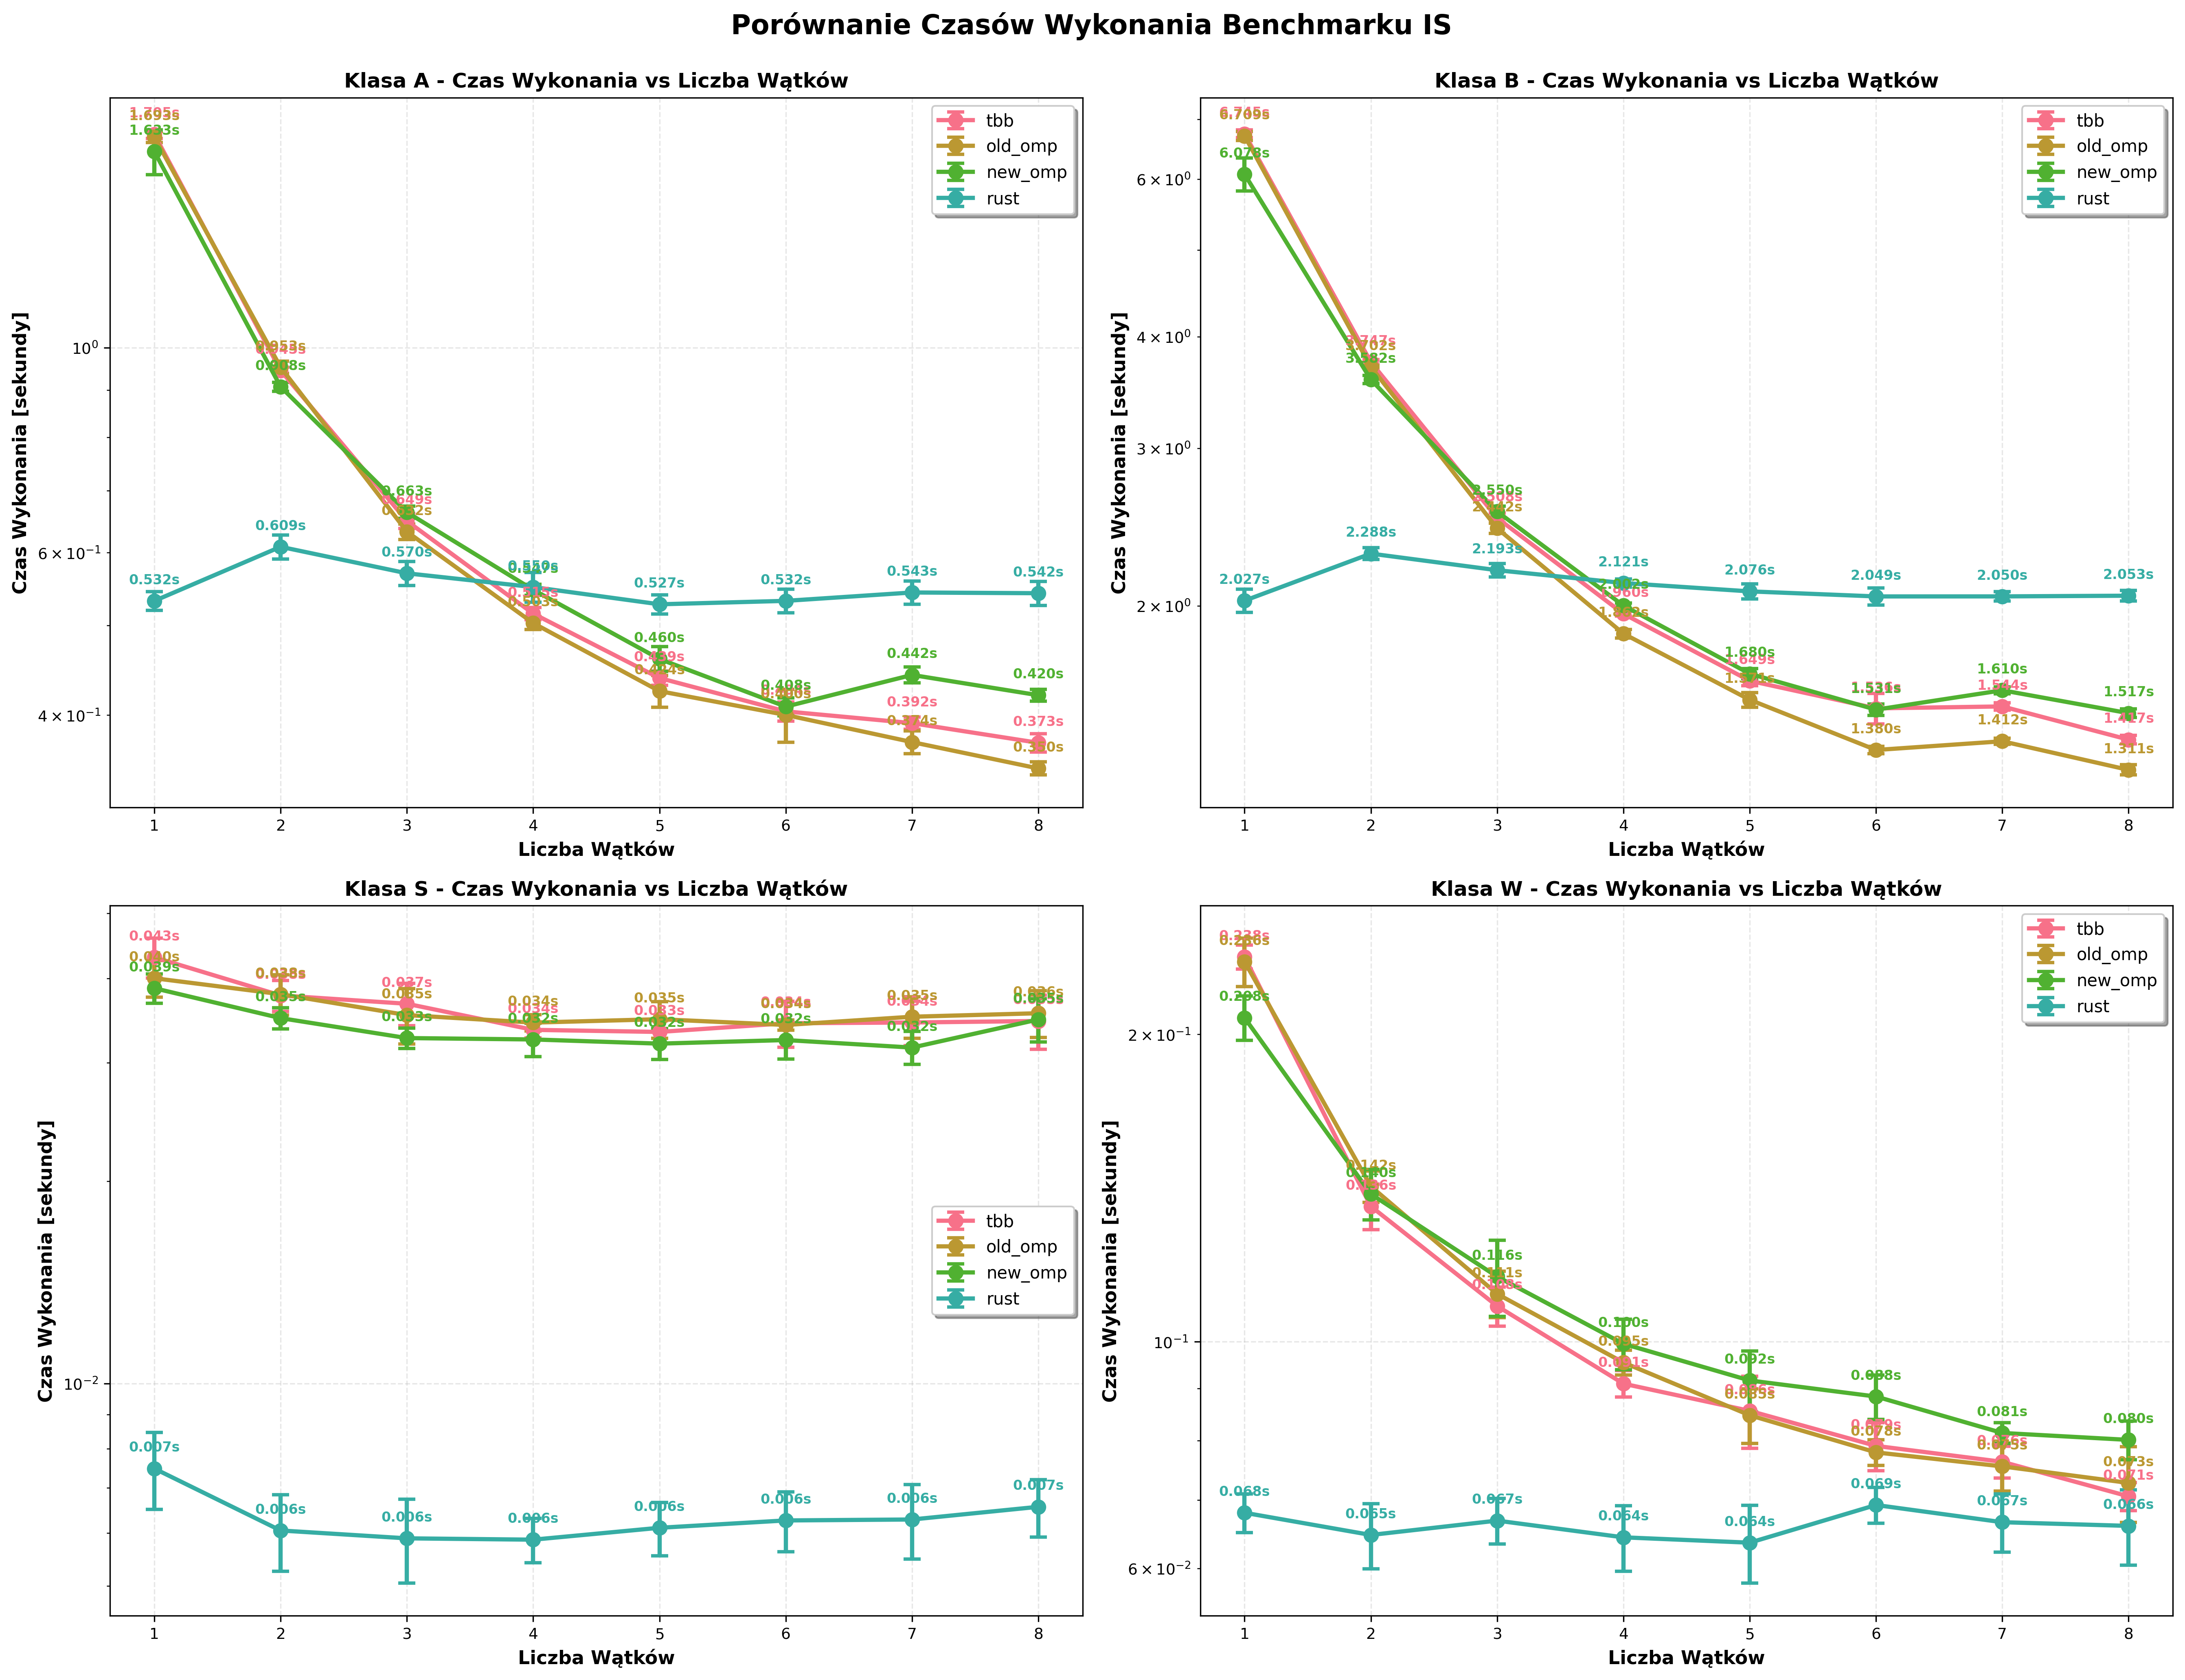
\includegraphics[width=0.9\textwidth]{analiza/images/parallel/is/x86/is_porownanie_czasow_wykonania.png}
    \caption{Porównanie czasów wykonania benchmarku IS dla klas S, W, A, B względem liczby użytych wątków}
    \label{is_porownanie_czasow_wykonania_x86}
\end{figure}
Analiza czasów wykonania - rysunek \ref{is_porownanie_czasow_wykonania_x86} ujawnia jednoznaczną przewagę implementacji Rust, która we wszystkich klasach problemu uzyskuje najniższe wartości czasów wykonania. Różnice te stają się szczególnie widoczne przy większej liczbie wątków. Dla przykładu, w klasie A przy ośmiu wątkach implementacja Rust osiąga czas około 0,542 sekundy, podczas gdy inne rozwiązania mieszczą się w zakresie 0,360-0,420 sekundy. Jeszcze wyraźniejsza dysproporcja występuje w klasie B, gdzie czas wykonania dla Rust wynosi około 2,05 sekundy, a dla pozostałych implementacji mieści się w przedziale 1,35-1,55 sekundy.

Implementacje różnią się istotnie pod względem charakterystyki skalowania wraz ze wzrostem liczby wątków. Implementacje \texttt{tbb}, \texttt{old\_omp} oraz \texttt{new\_omp} wykazują przewidywalny, choć ograniczony spadek czasu wykonania przy zwiększaniu liczby wątków. Największe zyski pojawiają się między 1 a 4 wątkami. Po przekroczeniu tego progu przyrosty stają się marginalne, a niekiedy nawet zauważalny jest niewielki wzrost czasu. W większości konfiguracji implementacja \texttt{tbb} okazuje się minimalnie szybsza od pozostałych, co może wskazywać na skuteczniejszą obsługę wątków w tej bibliotece.

Z kolei implementacja Rust prezentuje niemal całkowicie płaską charakterystykę czasową dla liczby wątków większej niż jeden. W klasach A i B można wręcz zaobserwować nieznaczne pogorszenie czasu wykonania przy przejściu z jednego do dwóch wątków.

Wyraźnie zarysowuje się różnica między większymi (A, B) a mniejszymi (S, W) klasami problemu. Dla klas A i B, które reprezentują bardziej wymagające obciążenia obliczeniowe, występują największe bezwzględne różnice czasów wykonania między Rust a pozostałymi implementacjami. Jednocześnie, implementacje \texttt{tbb}, \texttt{old\_omp} i \texttt{new\_omp} wykazują w tych klasach bardziej regularne i przewidywalne skalowanie, osiągając relatywnie największe przyspieszenia.

W przypadku klas S i W obserwowane różnice między implementacjami są mniej wyraźne. Czas wykonania zmienia się tu w sposób mniej przewidywalny, a przyrosty wydajności wynikające z równoległości są znacznie słabsze. W klasie W można jednak zauważyć agresywne skalowanie w implementacjach \texttt{tbb}, \texttt{old\_omp} i \texttt{new\_omp}, co może świadczyć o tym, że rozmiar problemu lepiej współgra z architekturą pamięci podręcznej procesora, co z kolei przekłada się na wzrost efektywności.

\begin{figure}[H]
    \centering
    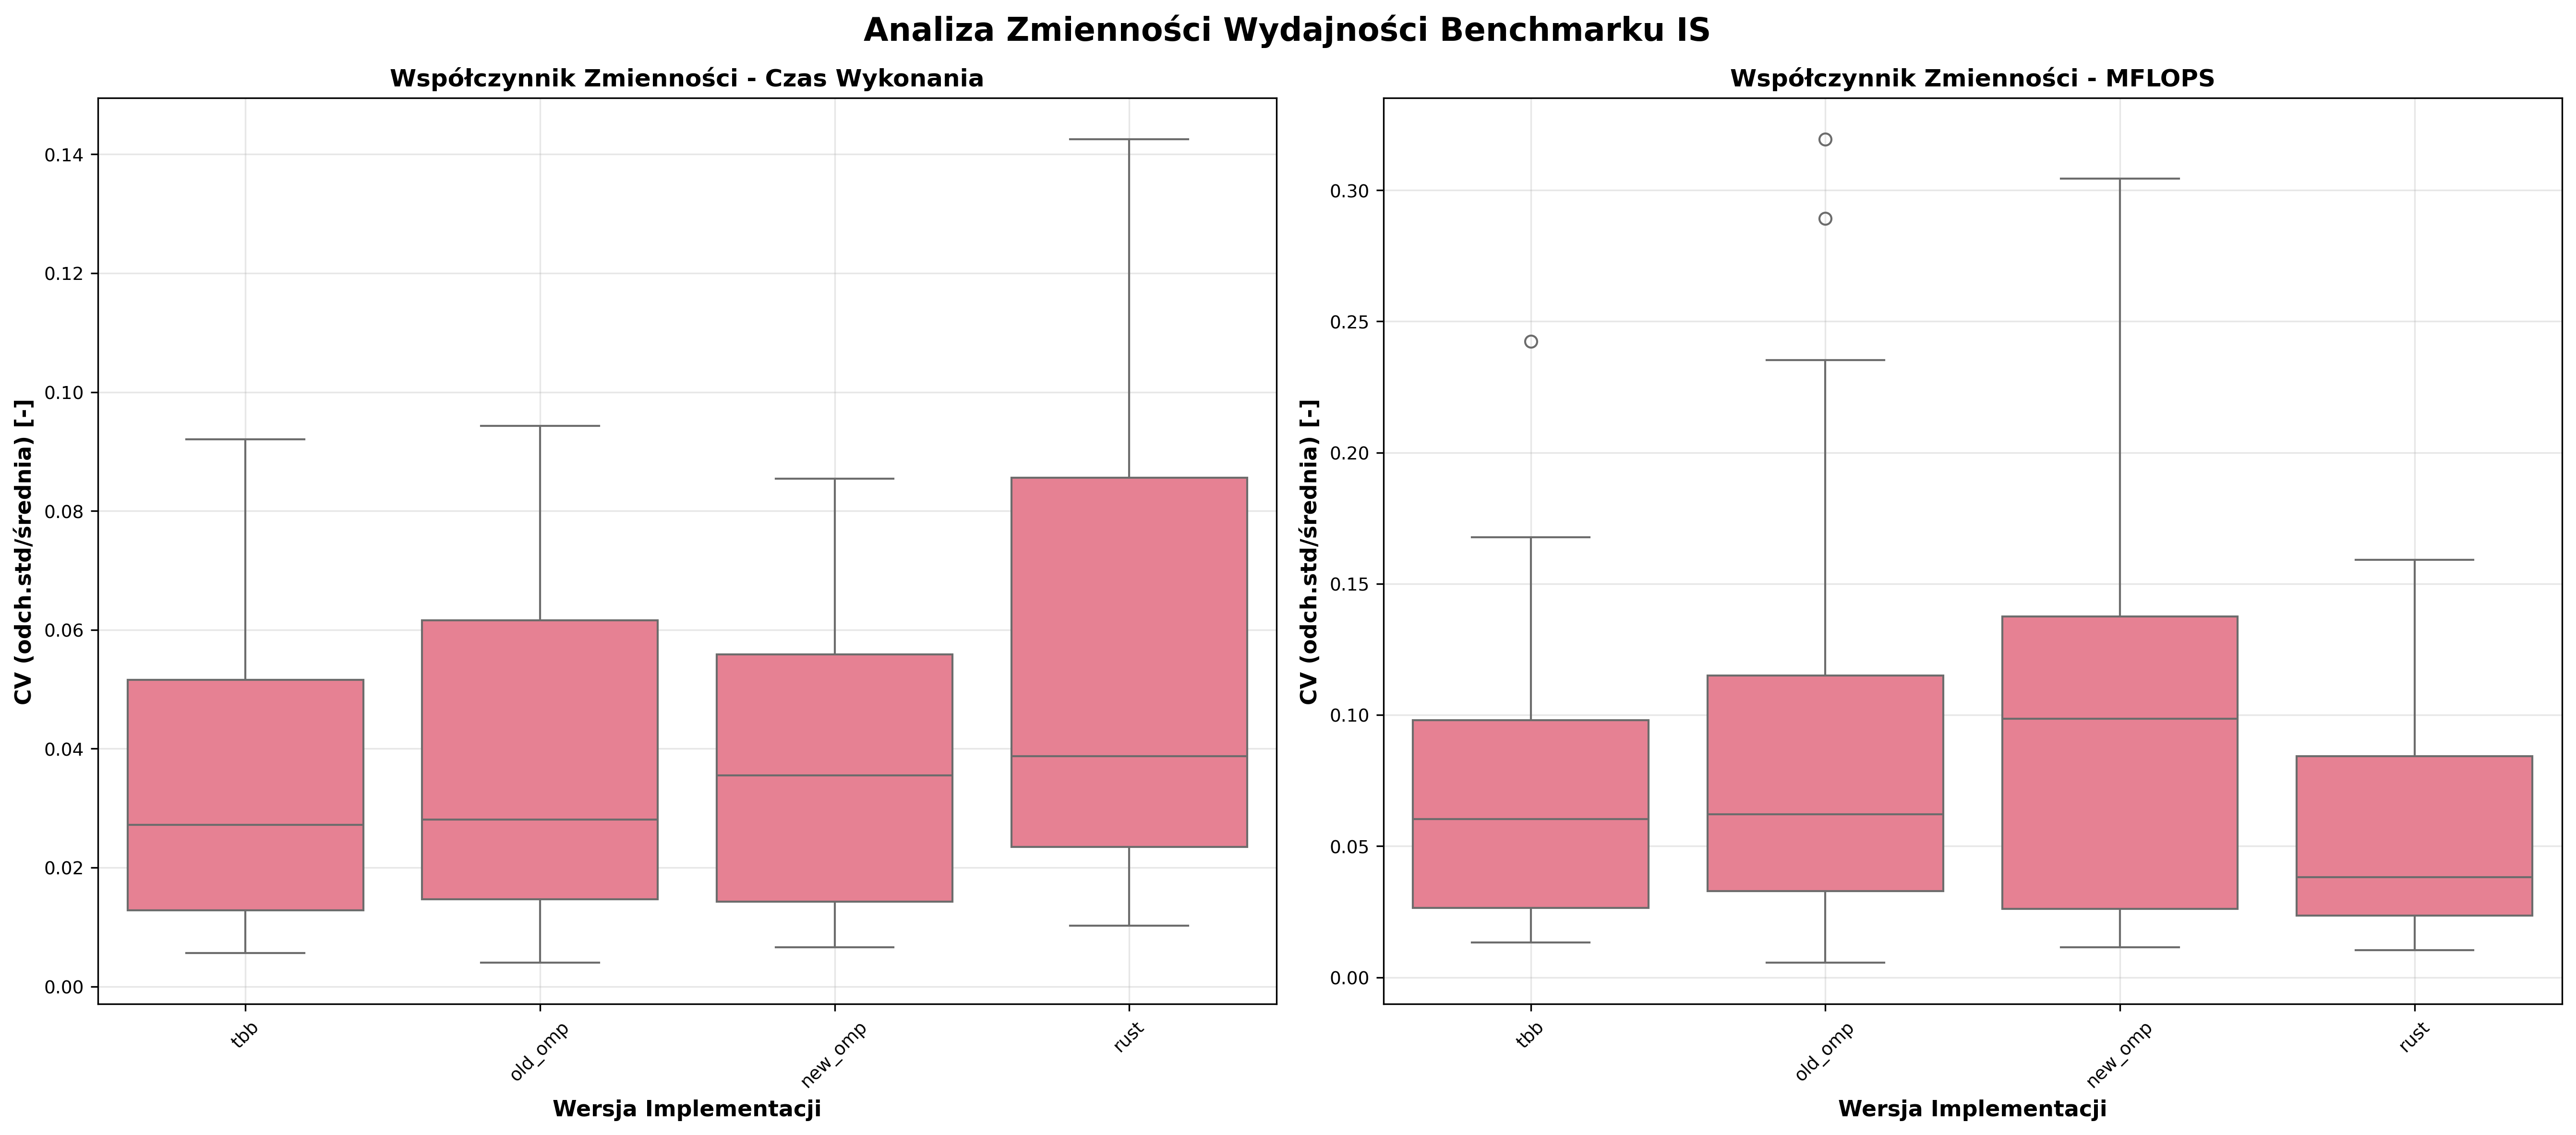
\includegraphics[width=0.9\textwidth]{analiza/images/parallel/is/x86/is_analiza_zmiennosci.png}
    \caption{Analiza zmienności czasów wykonania benchmarku IS dla klas S, W, A, B względem liczby użytych wątków}
    \label{is_analiza_zmiennosci_x86}
\end{figure}
\subsubsection{Stabilność czasu wykonania}
Pod względem zmienności czasów wykonania implementacja Rust wypada najsłabiej — osiąga najwyższą medianę współczynnika zmienności (około 0,04) i wykazuje szerszy rozrzut wyników, co wskazuje na większą podatność na losowe fluktuacje. Obecność licznych wartości odstających sugeruje występowanie okazjonalnych, znacznych odchyleń od typowych czasów wykonania, co może być związane z zarządzaniem wątkami bądź alokacją pamięci.

Implementacje \texttt{tbb}, \texttt{old\_omp} i \texttt{new\_omp} prezentują znacznie niższe i bardzo zbliżone wartości współczynnika zmienności, oscylujące wokół 0,025-0,03. Cechują się one także węższym zakresem wyników oraz mniejszą liczbą wartości odstających, co wskazuje na większą przewidywalność czasów wykonania i lepszą stabilność działania w środowisku wielowątkowym.

\subsubsection{Stabilność MFLOPS}
Pod względem zmienności MFLOPS najniższą medianę współczynnika zmienności (około 0,05) uzyskuje implementacja Rust, co oznacza, że pomimo dużych wahań czasów wykonania, osiągana wydajność obliczeniowa jest relatywnie stabilna.

Z drugiej strony, najwyższą medianę zmienności MFLOPS (około 0,10) osiąga implementacja \texttt{new\_omp}, co wskazuje na znacznie większe wahania wydajności w czasie. \texttt{tbb} i \texttt{old\_omp} plasują się w środku stawki, z wynikami na poziomie 0,06-0,07, przy czym \texttt{old\_omp} wykazuje więcej wartości odstających, co może świadczyć o większej podatności na lokalne anomalie wydajnościowe.


\begin{figure}[H]
    \centering
    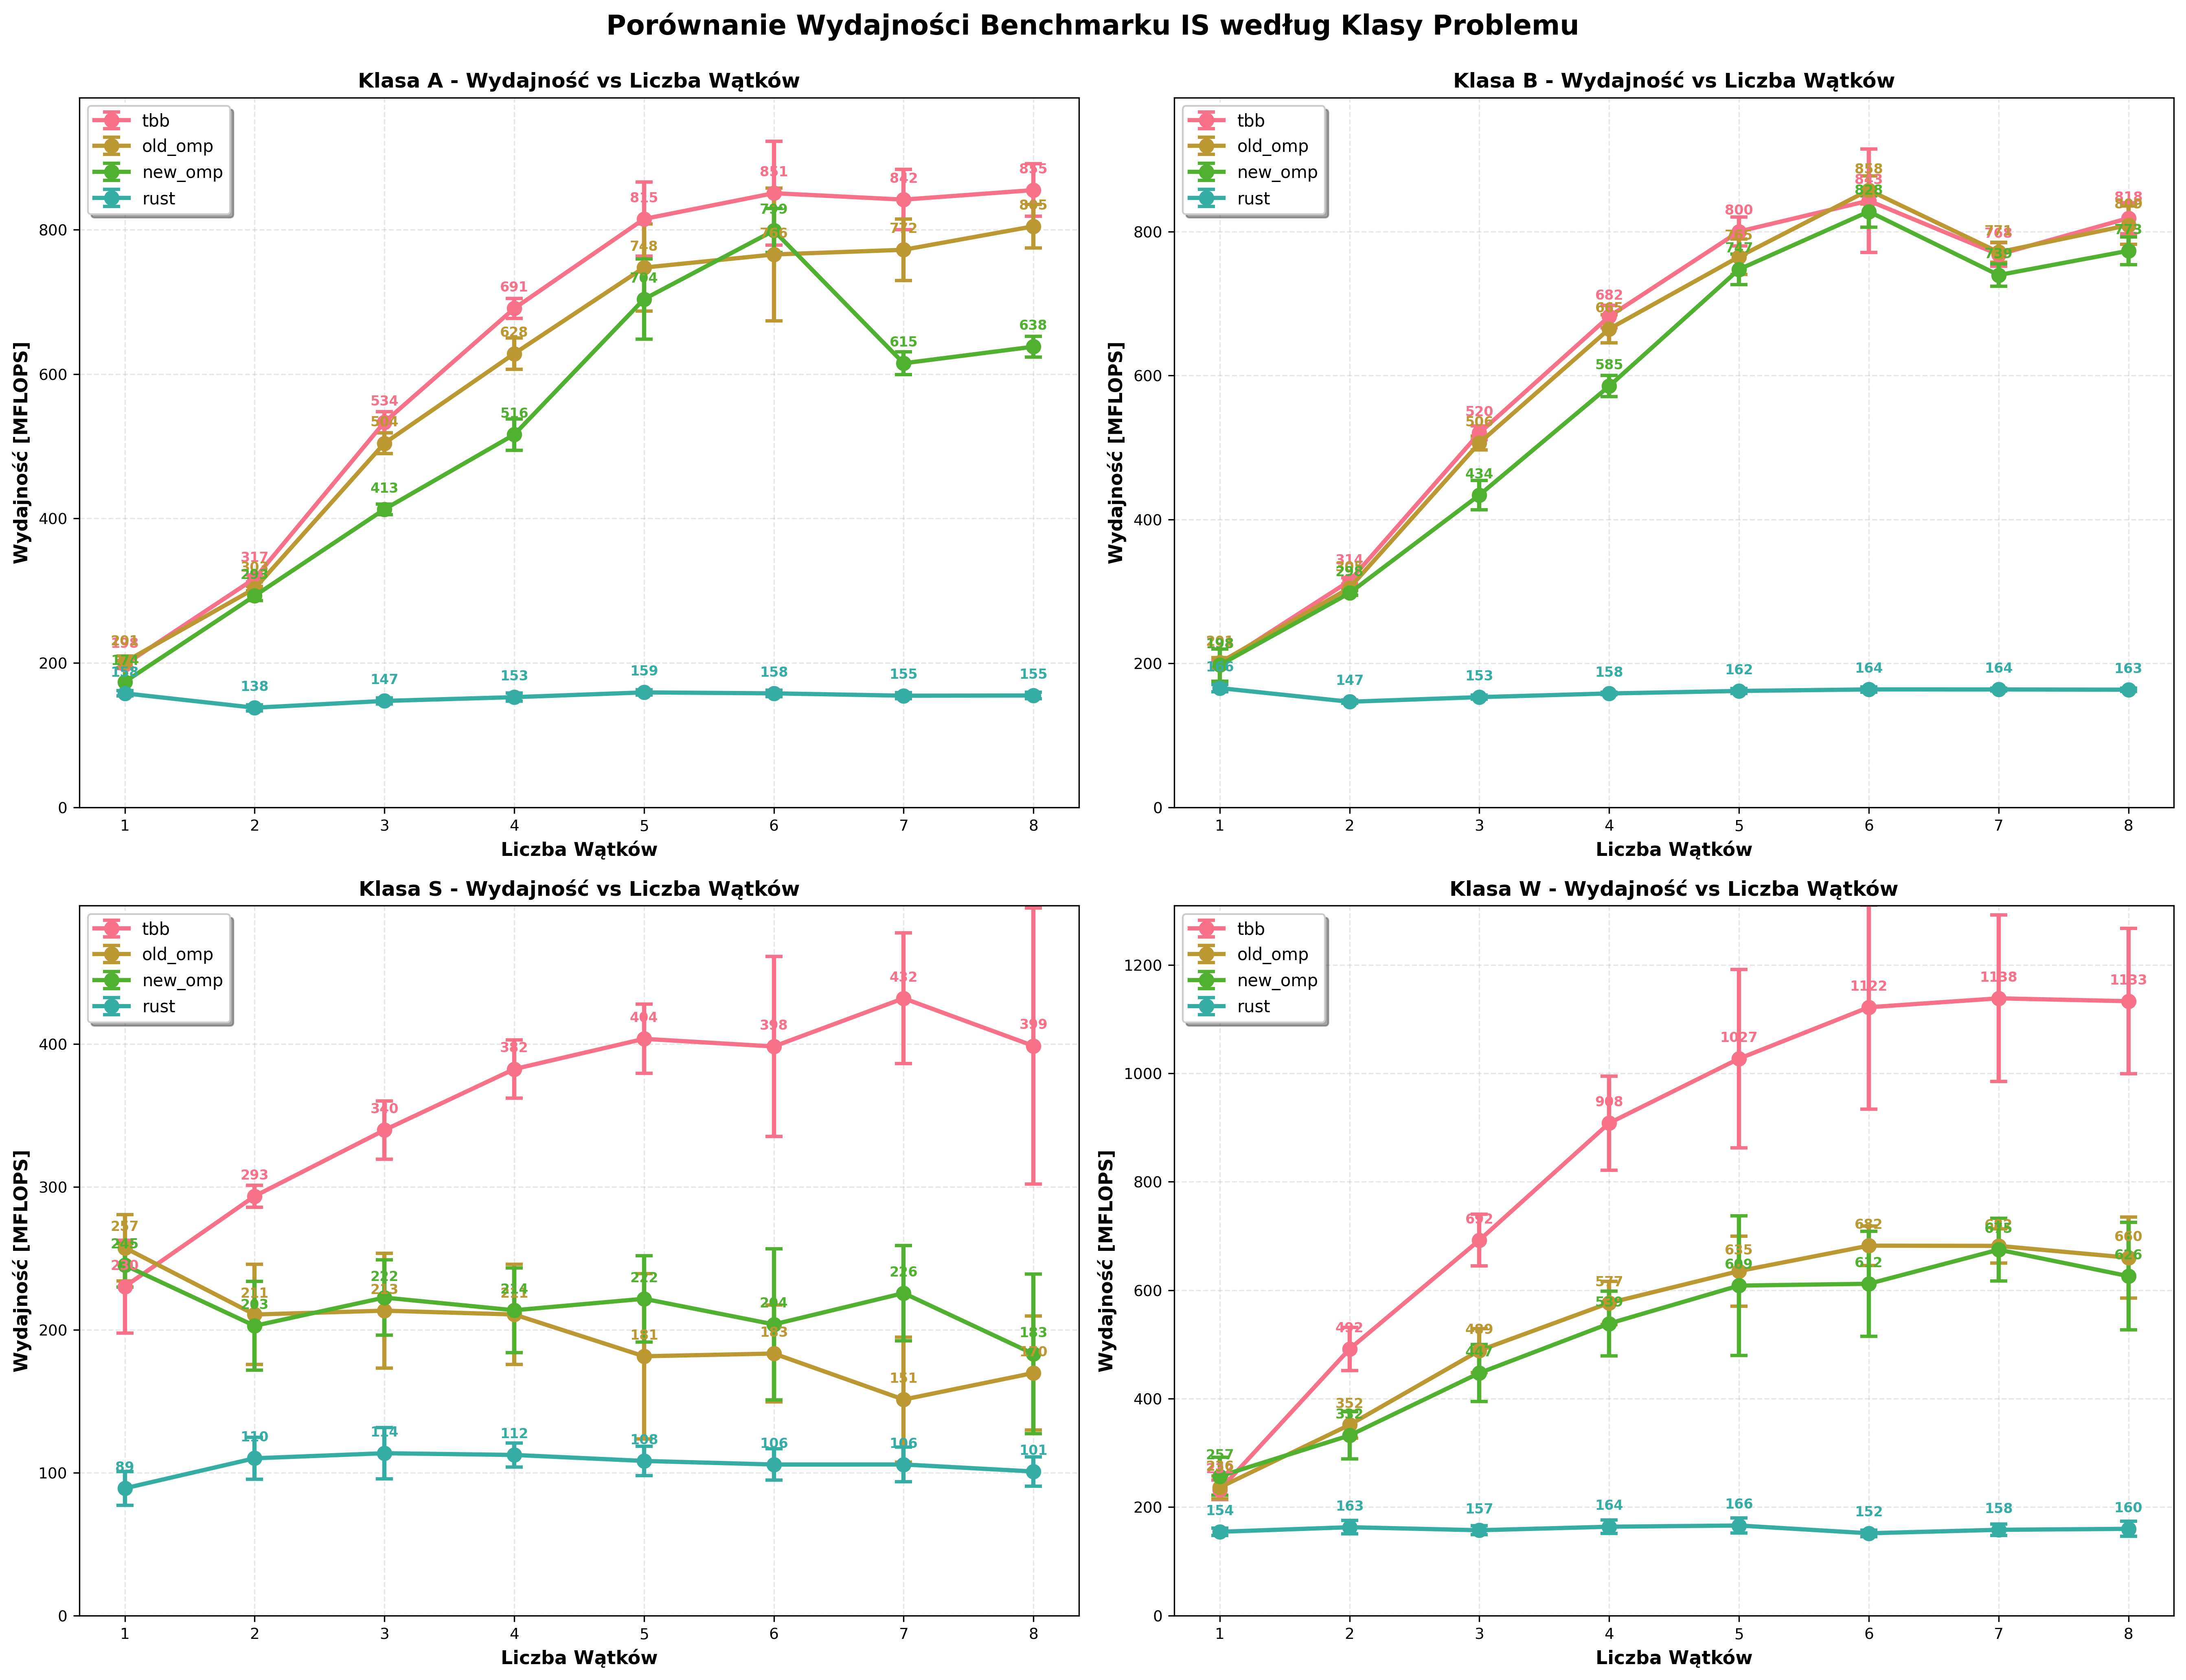
\includegraphics[width=0.9\textwidth]{analiza/images/parallel/is/x86/is_porownanie_wydajnosci.png}
    \caption{Porównanie wydajności benchmarku IS dla klas S, W, A, B względem liczby użytych wątków}
    \label{is_porownanie_wydajnosci_x86}
\end{figure}
Na wykresie - rysunek \ref{is_porownanie_wydajnosci_x86} rzuca się w oczy wyraźna różnica w charakterystyce wydajnościowej implementacji Rust względem pozostałych rozwiązań. Podczas gdy implementacje \texttt{tbb}, \texttt{old\_omp} i \texttt{new\_omp} wykazują wyraźny wzrost wydajności wraz ze wzrostem liczby wątków, implementacja Rust utrzymuje niemal stały poziom - około 150-160 MFLOPS w klasach A i B - niezależnie od stopnia zrównoleglenia.

W całej analizie dominuje implementacja \texttt{tbb}, która osiąga najwyższe wartości wydajności we wszystkich klasach problemu, szczególnie w klasie W, gdzie przewaga nad rozwiązaniami opartymi na OpenMP sięga kilkuset MFLOPS. Wydajność \texttt{tbb} wzrasta stabilnie do około \mbox{5-6} wątków, po czym osiąga linię prostą lub delikatnie spada, co jest typowym zjawiskiem przy nasyceniu zasobów systemowych.

Klasy problemowe różnią się nie tylko poziomem bezwzględnej wydajności, lecz także charakterem skalowania. Klasy A i B zachowują się podobnie - osiągają wysoką wydajność i~wykazują regularne skalowanie. Klasa S prezentuje niższe wartości i bardziej nieregularny przebieg, natomiast klasa W cechuje się najwyższymi szczytowymi wynikami, ale też największym zróżnicowaniem pomiędzy implementacjami.

\begin{figure}[!h]
    \centering
    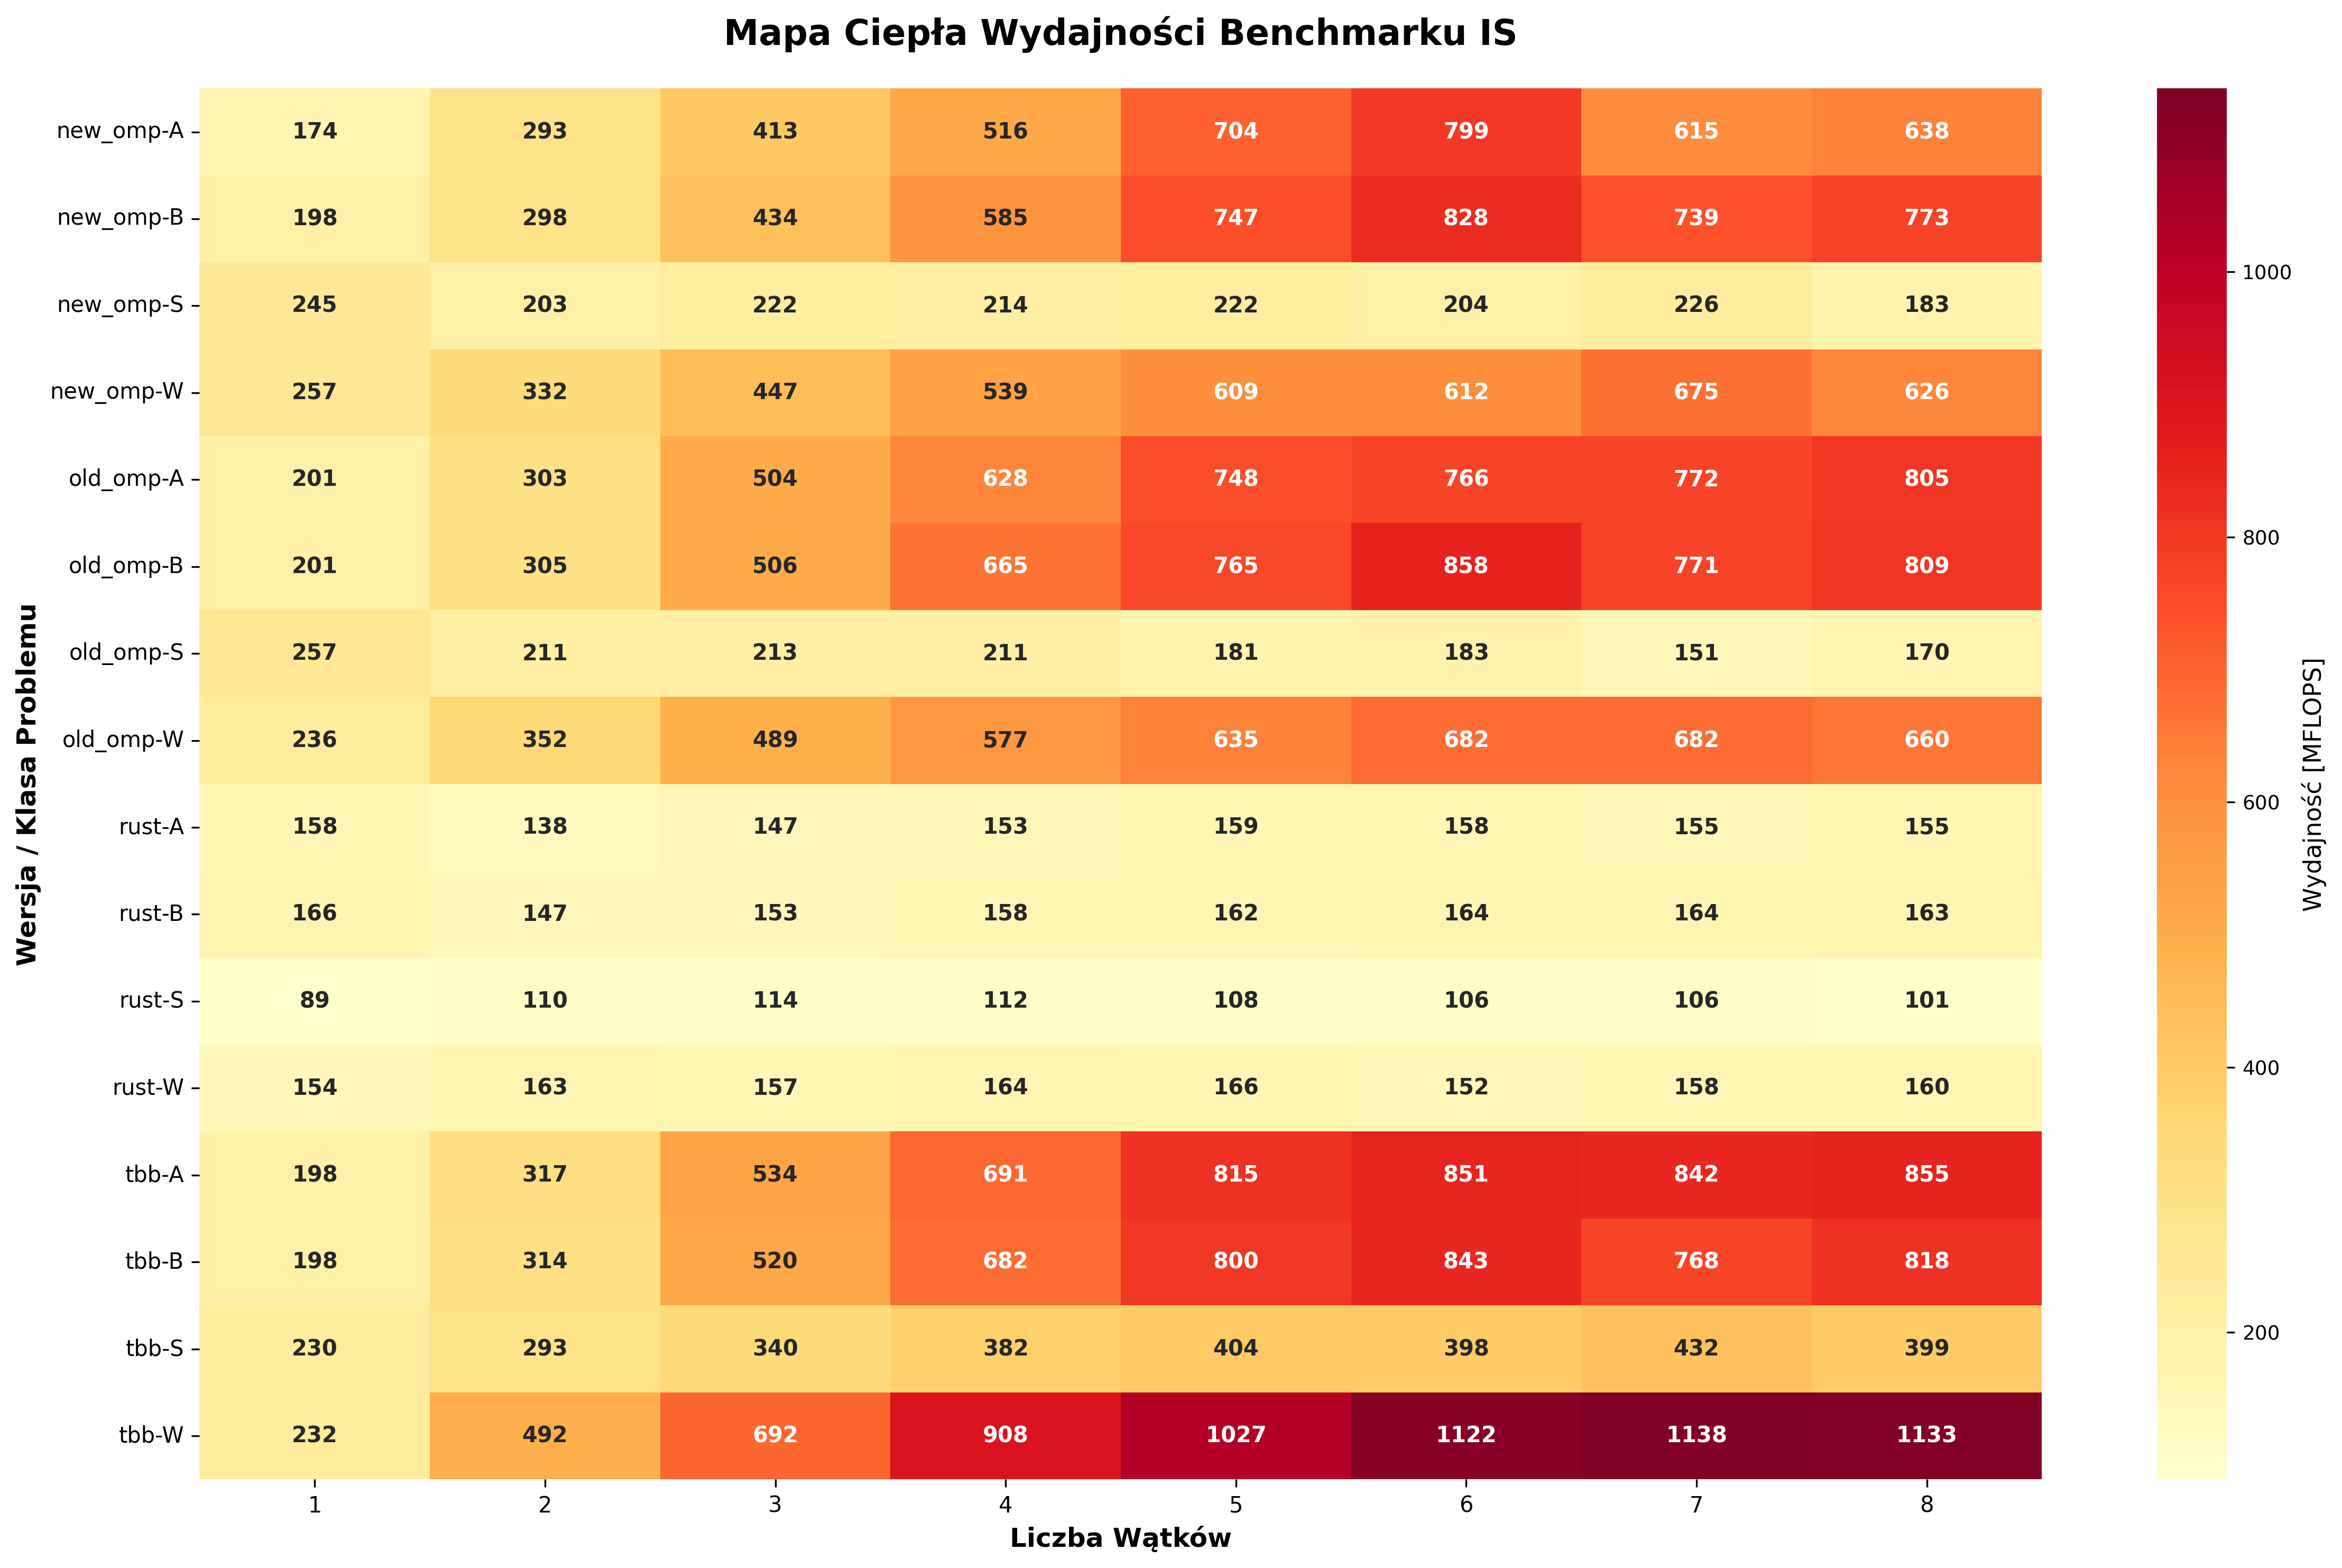
\includegraphics[width=0.9\textwidth]{analiza/images/parallel/is/x86/is_mapa_ciepla_wydajnosci.png}
    \caption{Mapa ciepła wydajności benchmarku IS dla klas S, W, A, B względem liczby użytych wątków}
    \label{is_heatmap_bench_wydajnosci_x86}
\end{figure}
Mapa ciepła - rysunek \ref{is_heatmap_bench_wydajnosci_x86} stanowi syntetyczne podsumowanie analizowanych danych. Najwyższe wartości wydajności skupiają się wokół implementacji \texttt{tbb}, szczególnie w klasie W i przy większej liczbie wątków. Z kolei implementacja Rust pozostaje na jednolitym, niskim poziomie niezależnie od klasy problemu czy liczby wątków. Klasa S wyraźnie odstaje od pozostałych pod względem niskiej wydajności, a dla większości implementacji najwyższe wartości osiągane są w zakresie 6-8 wątków, co potwierdza wnioski płynące z analizy skalowania.

\begin{figure}[H]
    \centering
    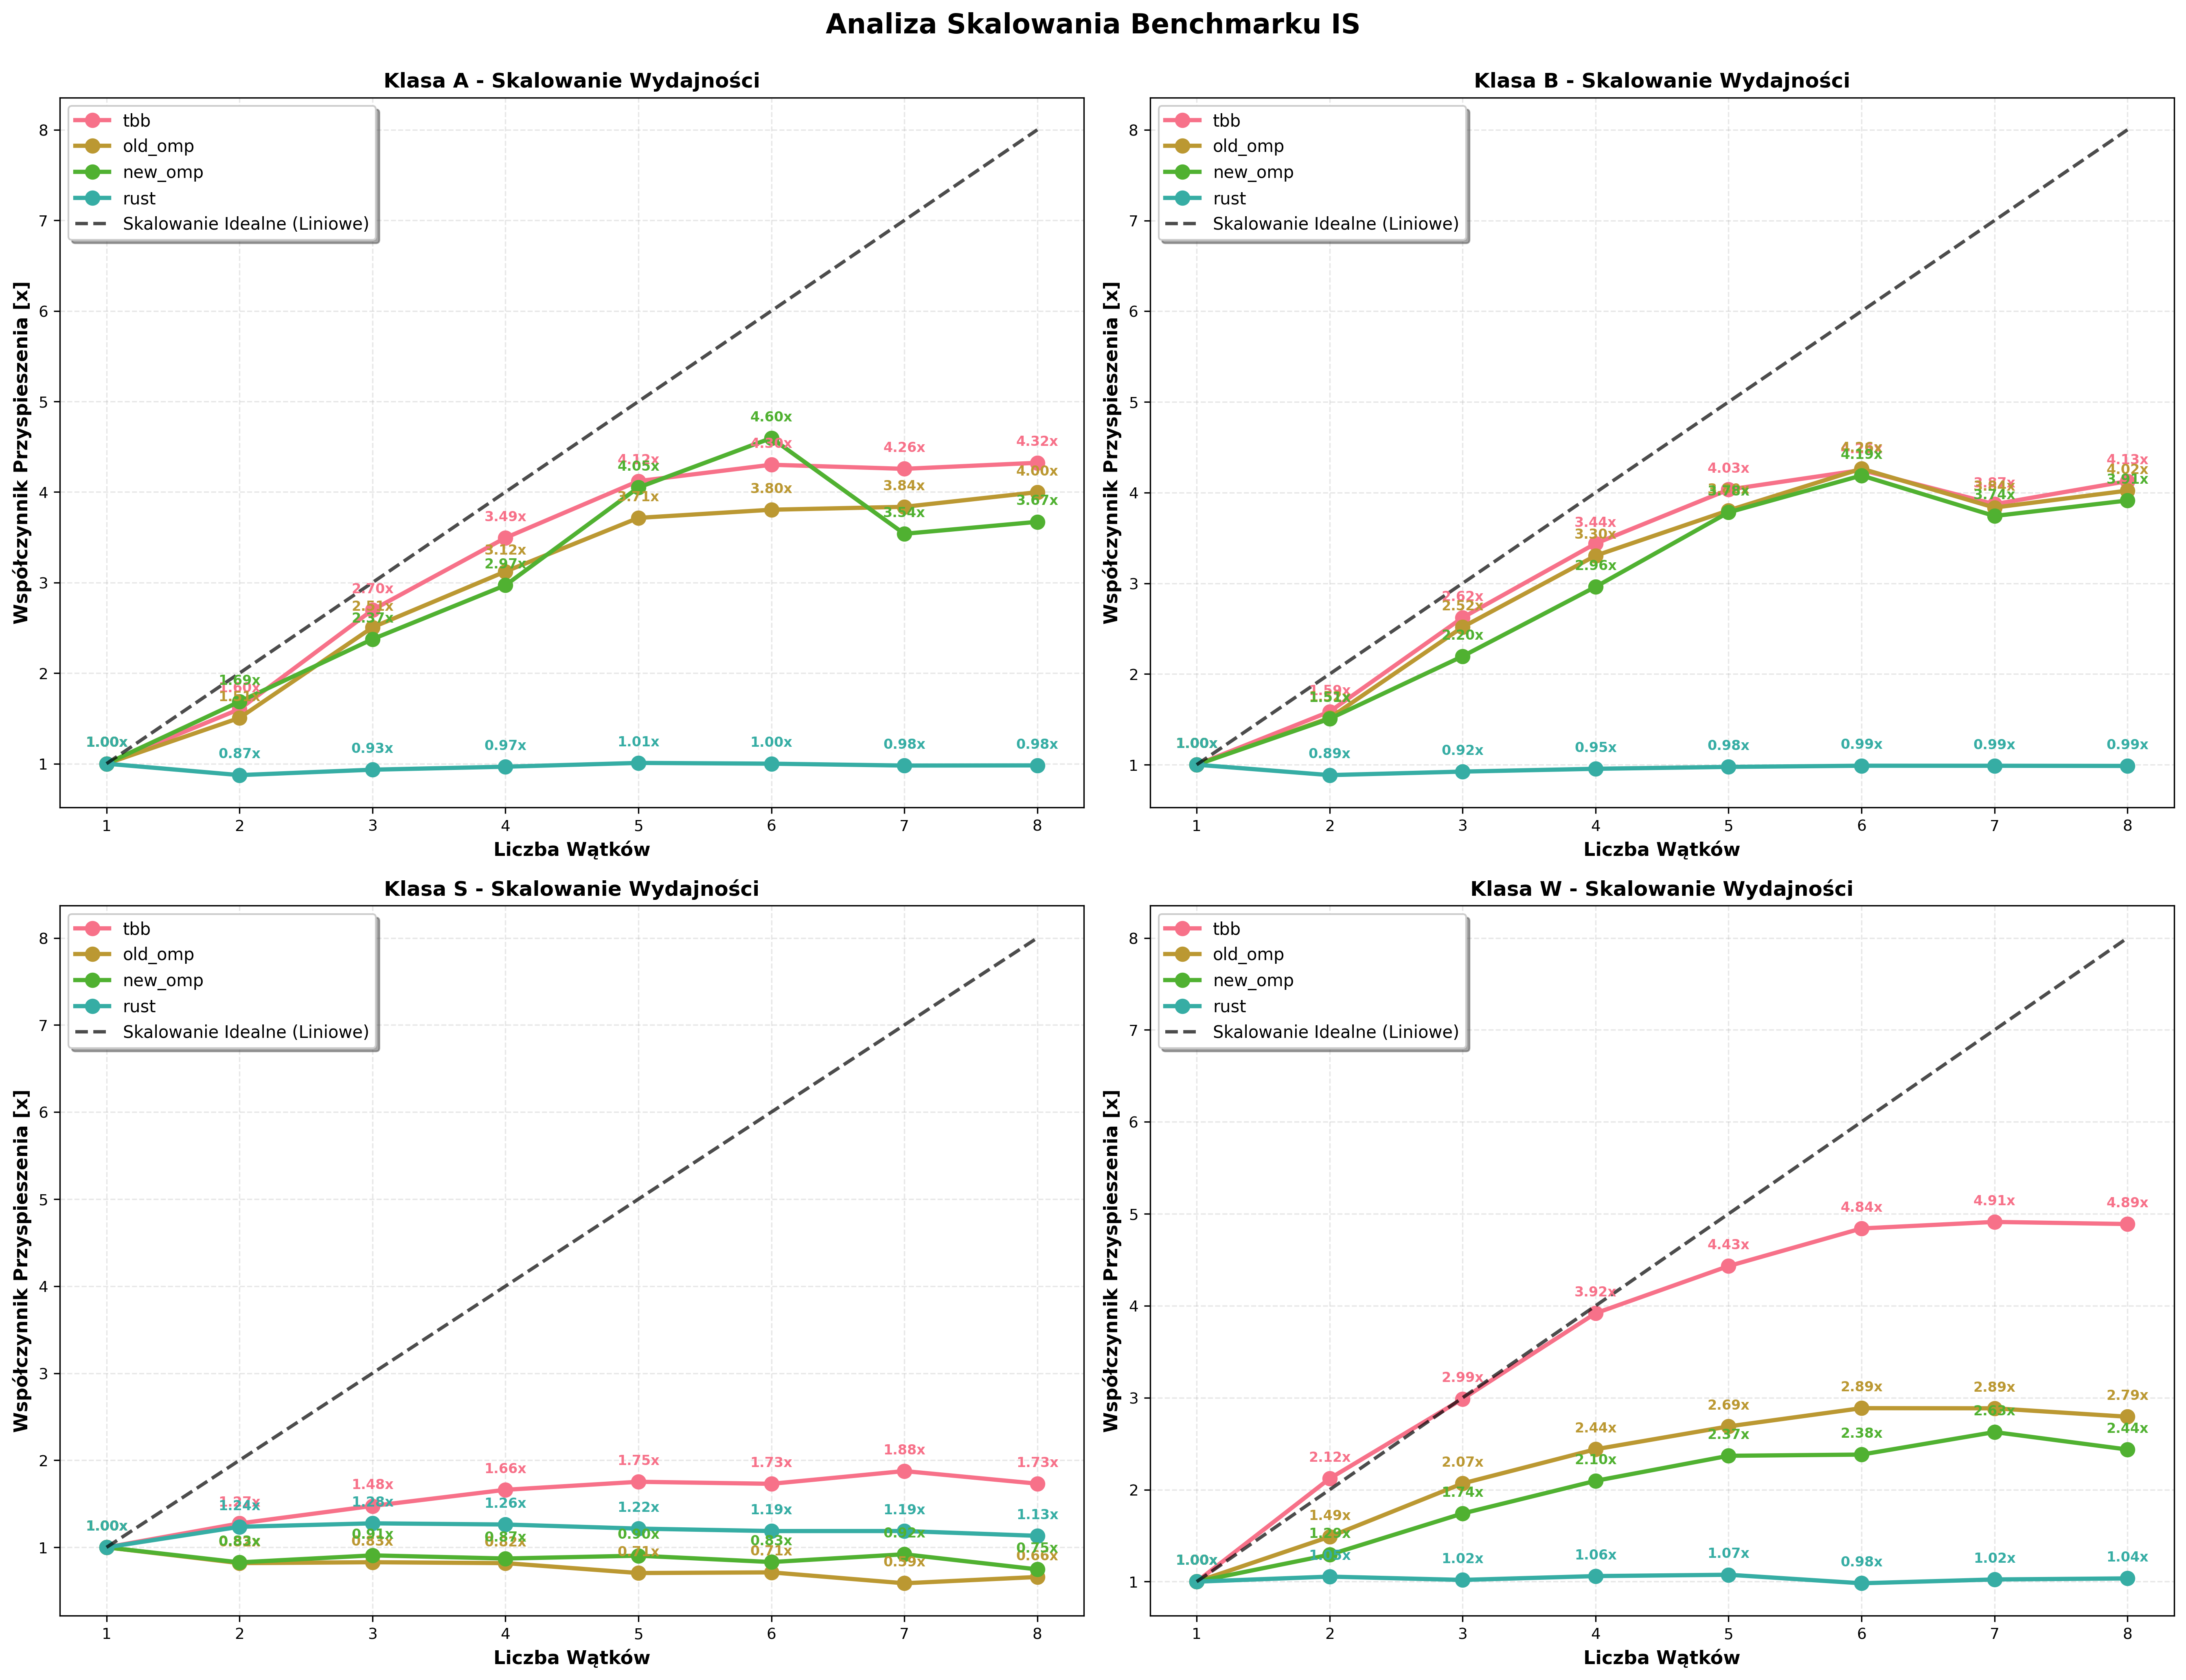
\includegraphics[width=0.9\textwidth]{analiza/images/parallel/is/x86/is_analiza_skalowania.png}
    \caption{Analiza skalowania benchmarku IS dla klas S, W, A, B względem liczby użytych wątków}
    \label{is_analiza_skalowania_x86}
\end{figure}
Wszystkie analizowane implementacje na wykresie - rysunek \ref{is_analiza_skalowania_x86} wykazują odchylenie od idealnego skalowania liniowego. Nawet najlepszy wynik - przyspieszenie rzędu 4,8x dla implementacji \texttt{tbb} w klasie W~przy 6-8 wątkach - stanowi zaledwie około 60\% teoretycznego maksimum. Spośród wszystkich badanych rozwiązań to właśnie \texttt{tbb} osiąga najefektywniejsze skalowanie we wszystkich klasach, szczególnie w klasie W, gdzie zdecydowanie dominuje nad konkurencją. Implementacje OpenMP (\texttt{old\_omp} i \texttt{new\_omp}) prezentują umiarkowane przyspieszenia, rzędu 3,8-4,3x w większych klasach problemowych (A i B), natomiast Rust praktycznie nie skaluje się wcale - współczynnik przyspieszenia oscyluje wokół 1, niezależnie od liczby wątków. Skalowanie silnie zależy również od klasy problemu. Klasy A i B charakteryzują się najbardziej efektywnym, choć wciąż dalekim od idealnego, wykorzystaniem równoległości (do około 4,6x). Klasa S wypada najsłabiej, nie przekraczając przyspieszenia 2x, co wynika z małej skali problemu niedostosowanej do architektury wielowątkowej. W klasie W obserwujemy najwyższe zróżnicowanie między implementacjami, przy czym \texttt{tbb} wyraźnie się wyróżnia. Dla większości implementacji punkt nasycenia wydajności przypada na 5-6 wątków, po czym następuje stabilizacja lub lekki spadek. Wskazuje to na osiągnięcie limitów przepustowości pamięci lub narzutów związanych z~synchronizacją w środowisku wielowątkowym.
%------------------------------
%------------------------------

\subsection{Wyniki profilowania wydajności - platforma ARM64}
Aby lepiej zrozumieć charakterystyki pamięciowe testowanych implementacji benchmarku IS, przeprowadzono analizę zużycia pamięci, błędów stron pamięci oraz mechanizmu ich odzyskiwania. Wnioski wyciągnięto na podstawie trzech grup wykresów: bezwzględnych wartości \mbox{(rys. \ref{is_porownanie_zuzycia_pamieci})}, porównania względnego względem \texttt{old\_omp} (rys. \ref{is_analiza_wzgledem_old_omp}) oraz kompromisów między metrykami \mbox{(rys. \ref{is_kompromisy_pamiec_bledy})}.
\begin{figure}[!h]
    \centering
    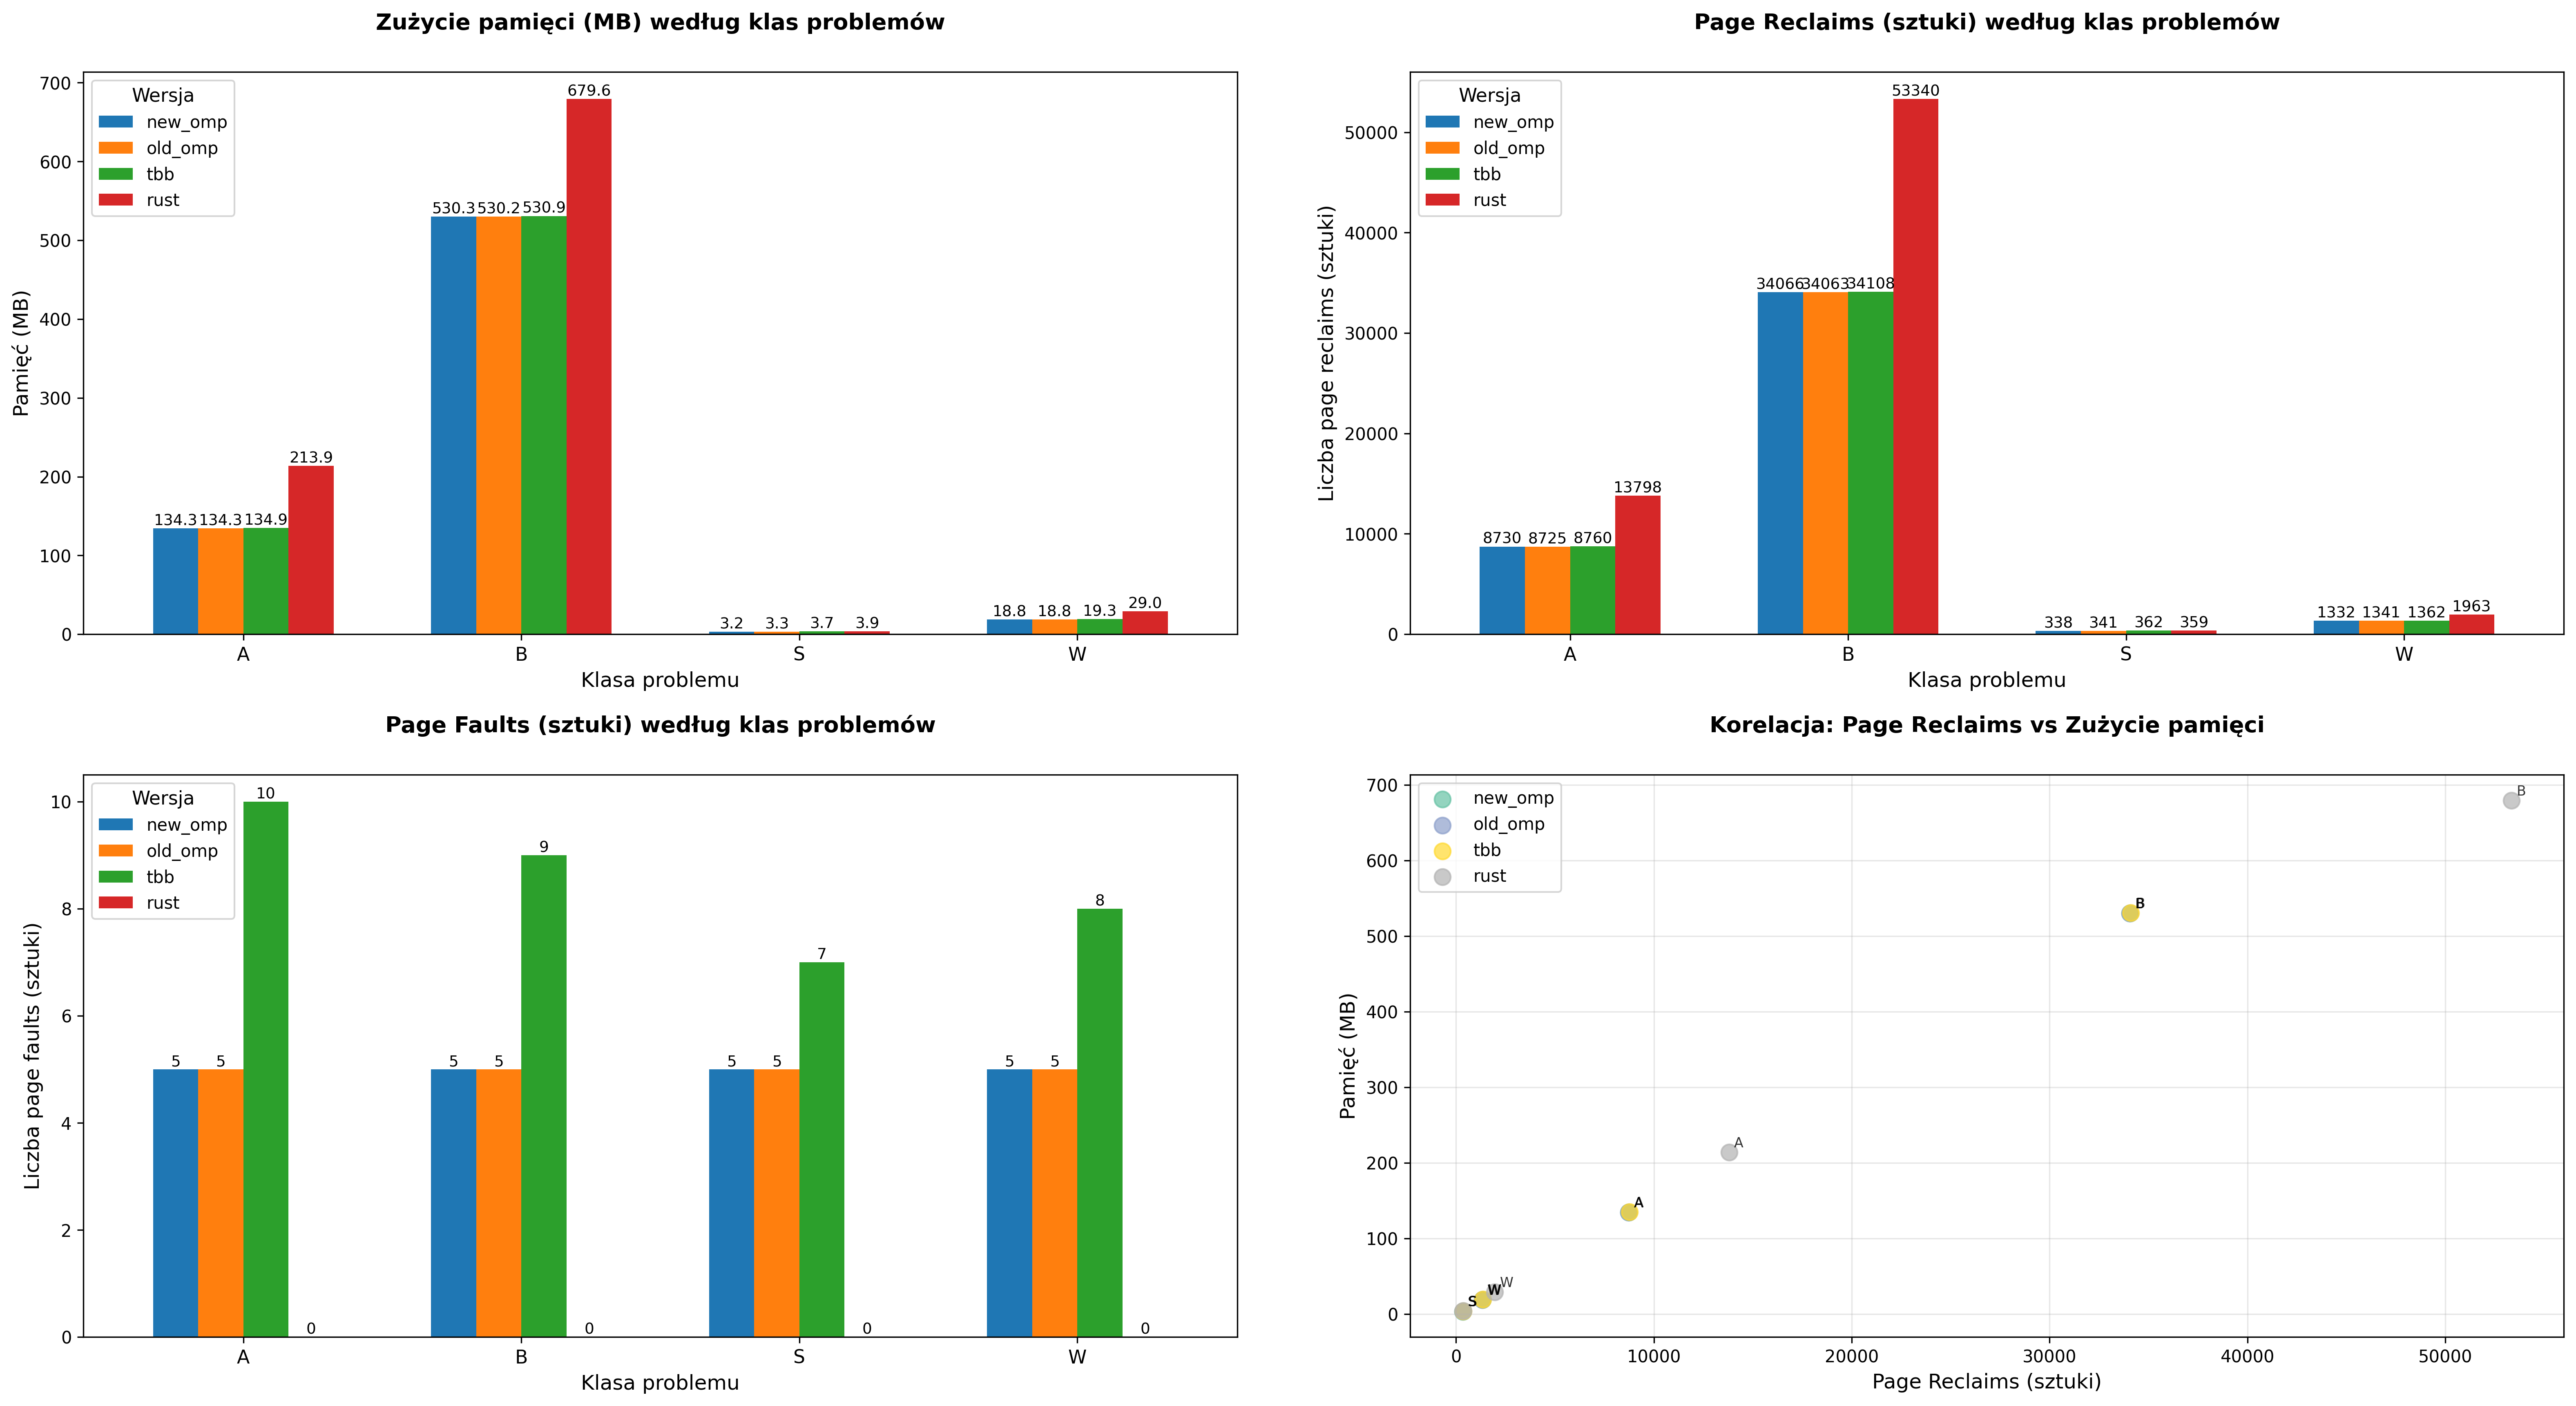
\includegraphics[width=0.9\textwidth]{analiza/images/parallel/is/arm/chart_01_memory_comparison.png}
    \caption{Profilowanie wydajności benchmarku IS dla klas S, W, A, B względem liczby użytych wątków}
    \label{is_porownanie_zuzycia_pamieci}
\end{figure}
\subsubsection{Zużycie pamięci i błędy stron}
Wykresy w górnym rzędzie przedstawiają bezwzględne zużycie pamięci oraz liczbę odzyskanych stron pamięci:
\begin{itemize}
    \item Największe zużycie pamięci odnotowano dla implementacji \texttt{rust}, osiągając 213,9 MB (klasa A) oraz 679,6 MB (klasa B). W pozostałych implementacjach (\texttt{new\_omp}, \texttt{old\_omp}, \texttt{tbb}) wartości te były niemal identyczne (np. ~134 MB w klasie A i ~530 MB w klasie B).
    \item Analogicznie, \texttt{rust} odzyskuje najwięcej stron, osiągając ponad 53 tysiące operacji w klasie B, co jest o ponad 50\% więcej niż w pozostałych wersjach. Sugeruje to intensywniejsze wykorzystanie dynamicznego zarządzania pamięcią lub częstsze zwalnianie obszarów.
    \item W zakresie błędów stron, \texttt{rust} jako jedyna implementacja nie generuje żadnych błędów stron (0 sztuk we wszystkich klasach), co potwierdza jej deterministyczne podejście do alokacji pamięci.
    \item Wersje \texttt{new\_omp} i \texttt{old\_omp} utrzymują stabilny poziom błędów (5 sztuk we wszystkich klasach), natomiast \texttt{tbb} wykazuje wyraźnie wyższy poziom błędów - od 7 do 10 sztuk.
\end{itemize}
W prawym dolnym wykresie zaprezentowano korelację między zużyciem pamięci a liczbą oddanych stron. Wykres ujawnia wyraźną korelację dodatnią - implementacje i klasy, które zużywają więcej pamięci, zwalniają również więcej stron z pamięcią, co wynika z konieczności intensywniejszej obsługi zarządzania pamięcią operacyjną.

\begin{figure}[!h]
    \centering
    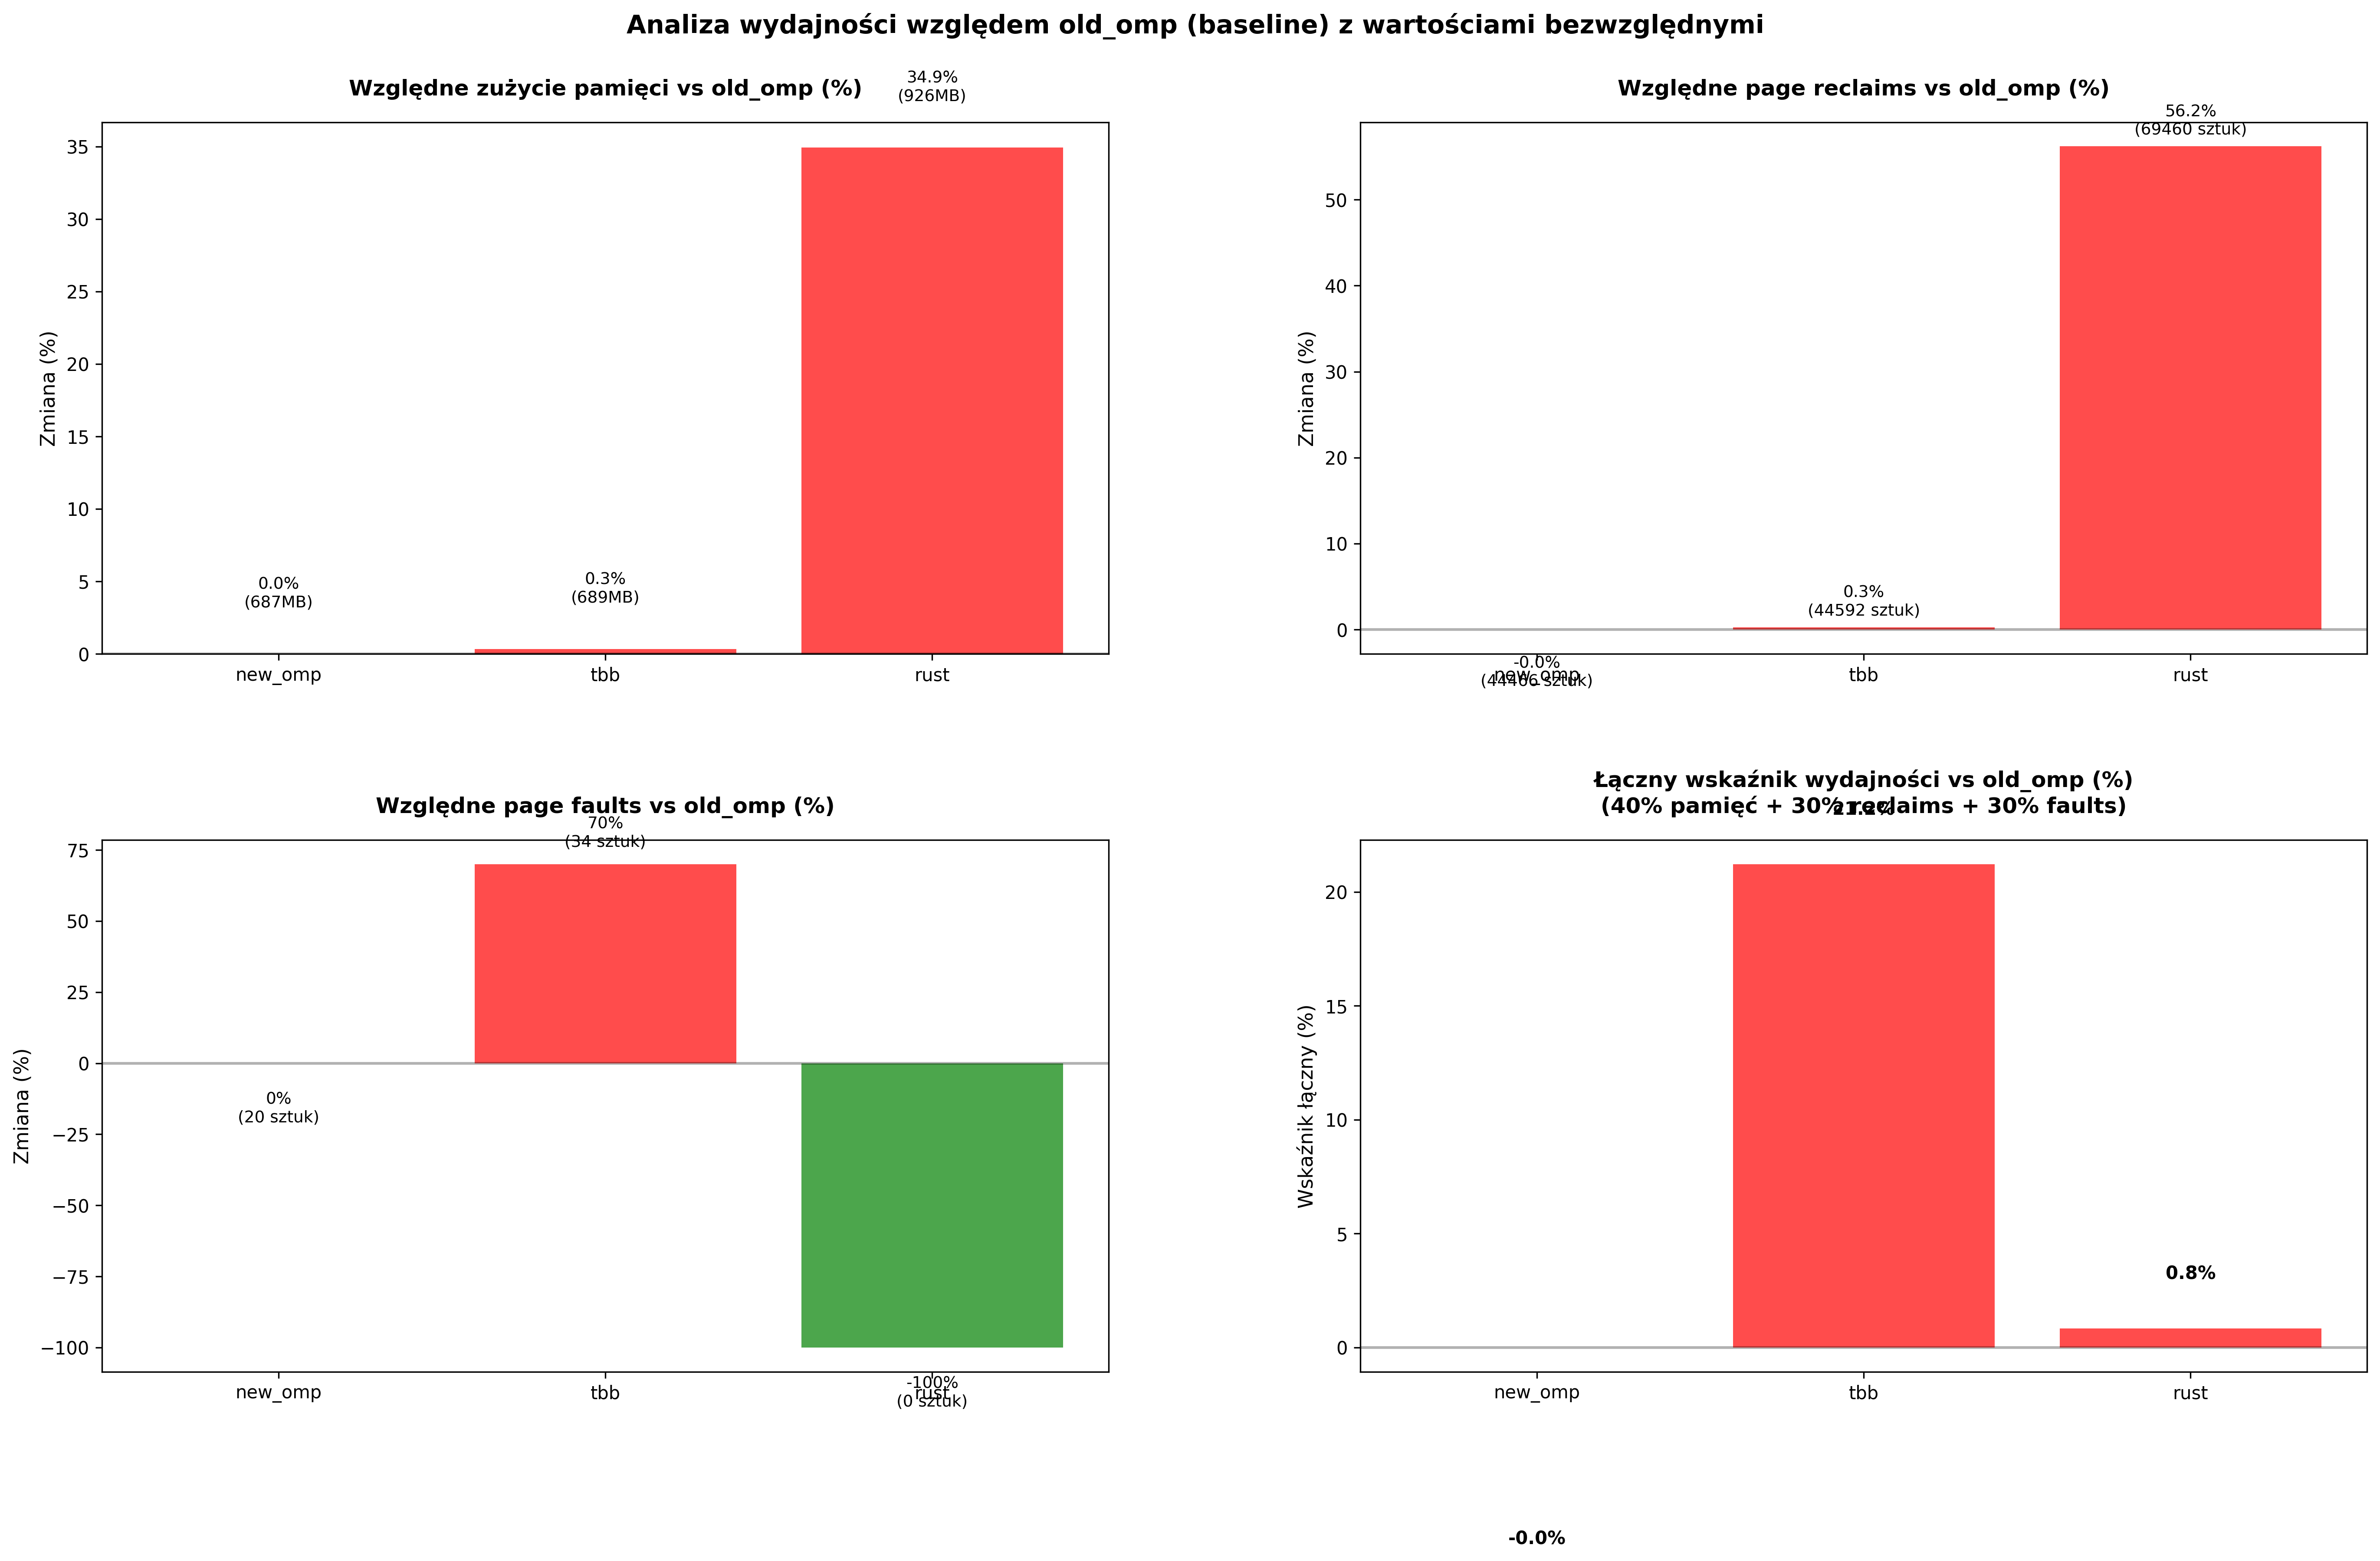
\includegraphics[width=0.9\textwidth]{analiza/images/parallel/is/arm/chart_05_performance_ratios.png}
    \caption{Analiza wydajności względem \texttt{old\_omp} (punkt odniesienia) z wartościami bezwzględnymi}
    \label{is_analiza_wzgledem_old_omp}
\end{figure}
Wykres ten - rysunek \ref{is_analiza_wzgledem_old_omp} przedstawia zmiany procentowe trzech kluczowych metryk względem wersji odniesienia (\texttt{old\_omp}):
\begin{itemize}
    \item Zużycie pamięci: \texttt{new\_omp} nie różni się w ogóle od wersji odniesienia (0\%), \texttt{tbb} wykazuje jedynie symboliczny wzrost (0,3\%), natomiast \texttt{rust} zużywa aż 34,9\% więcej pamięci.
    \item Odzyskiwanie stron pamięci: \texttt{rust} generuje aż 56,2\% więcej operacji odzyskania niż \texttt{old\_omp}, co stanowi znaczące obciążenie podsystemu pamięci.
    \item Błędy stron: \texttt{rust} jako jedyna implementacja całkowicie je eliminuje (-100\% względem \texttt{old\_omp}), co jest jej największym atutem oraz potwierdza założenia co do mechanizmów języka.
    \item Wskaźnik zbiorczy (ważony: 40\% pamięć + 30\% reclaims + 30\% faults) wskazuje, że jedynie \texttt{tbb} osiąga nieznaczną przewagę względem wersji bazowej (+0,8\%), natomiast \texttt{rust} wypada niekorzystnie pomimo doskonałej obsługi błędów, głównie przez nadmierne zużycie pamięci.
\end{itemize}



\begin{figure}[!h]
    \centering
    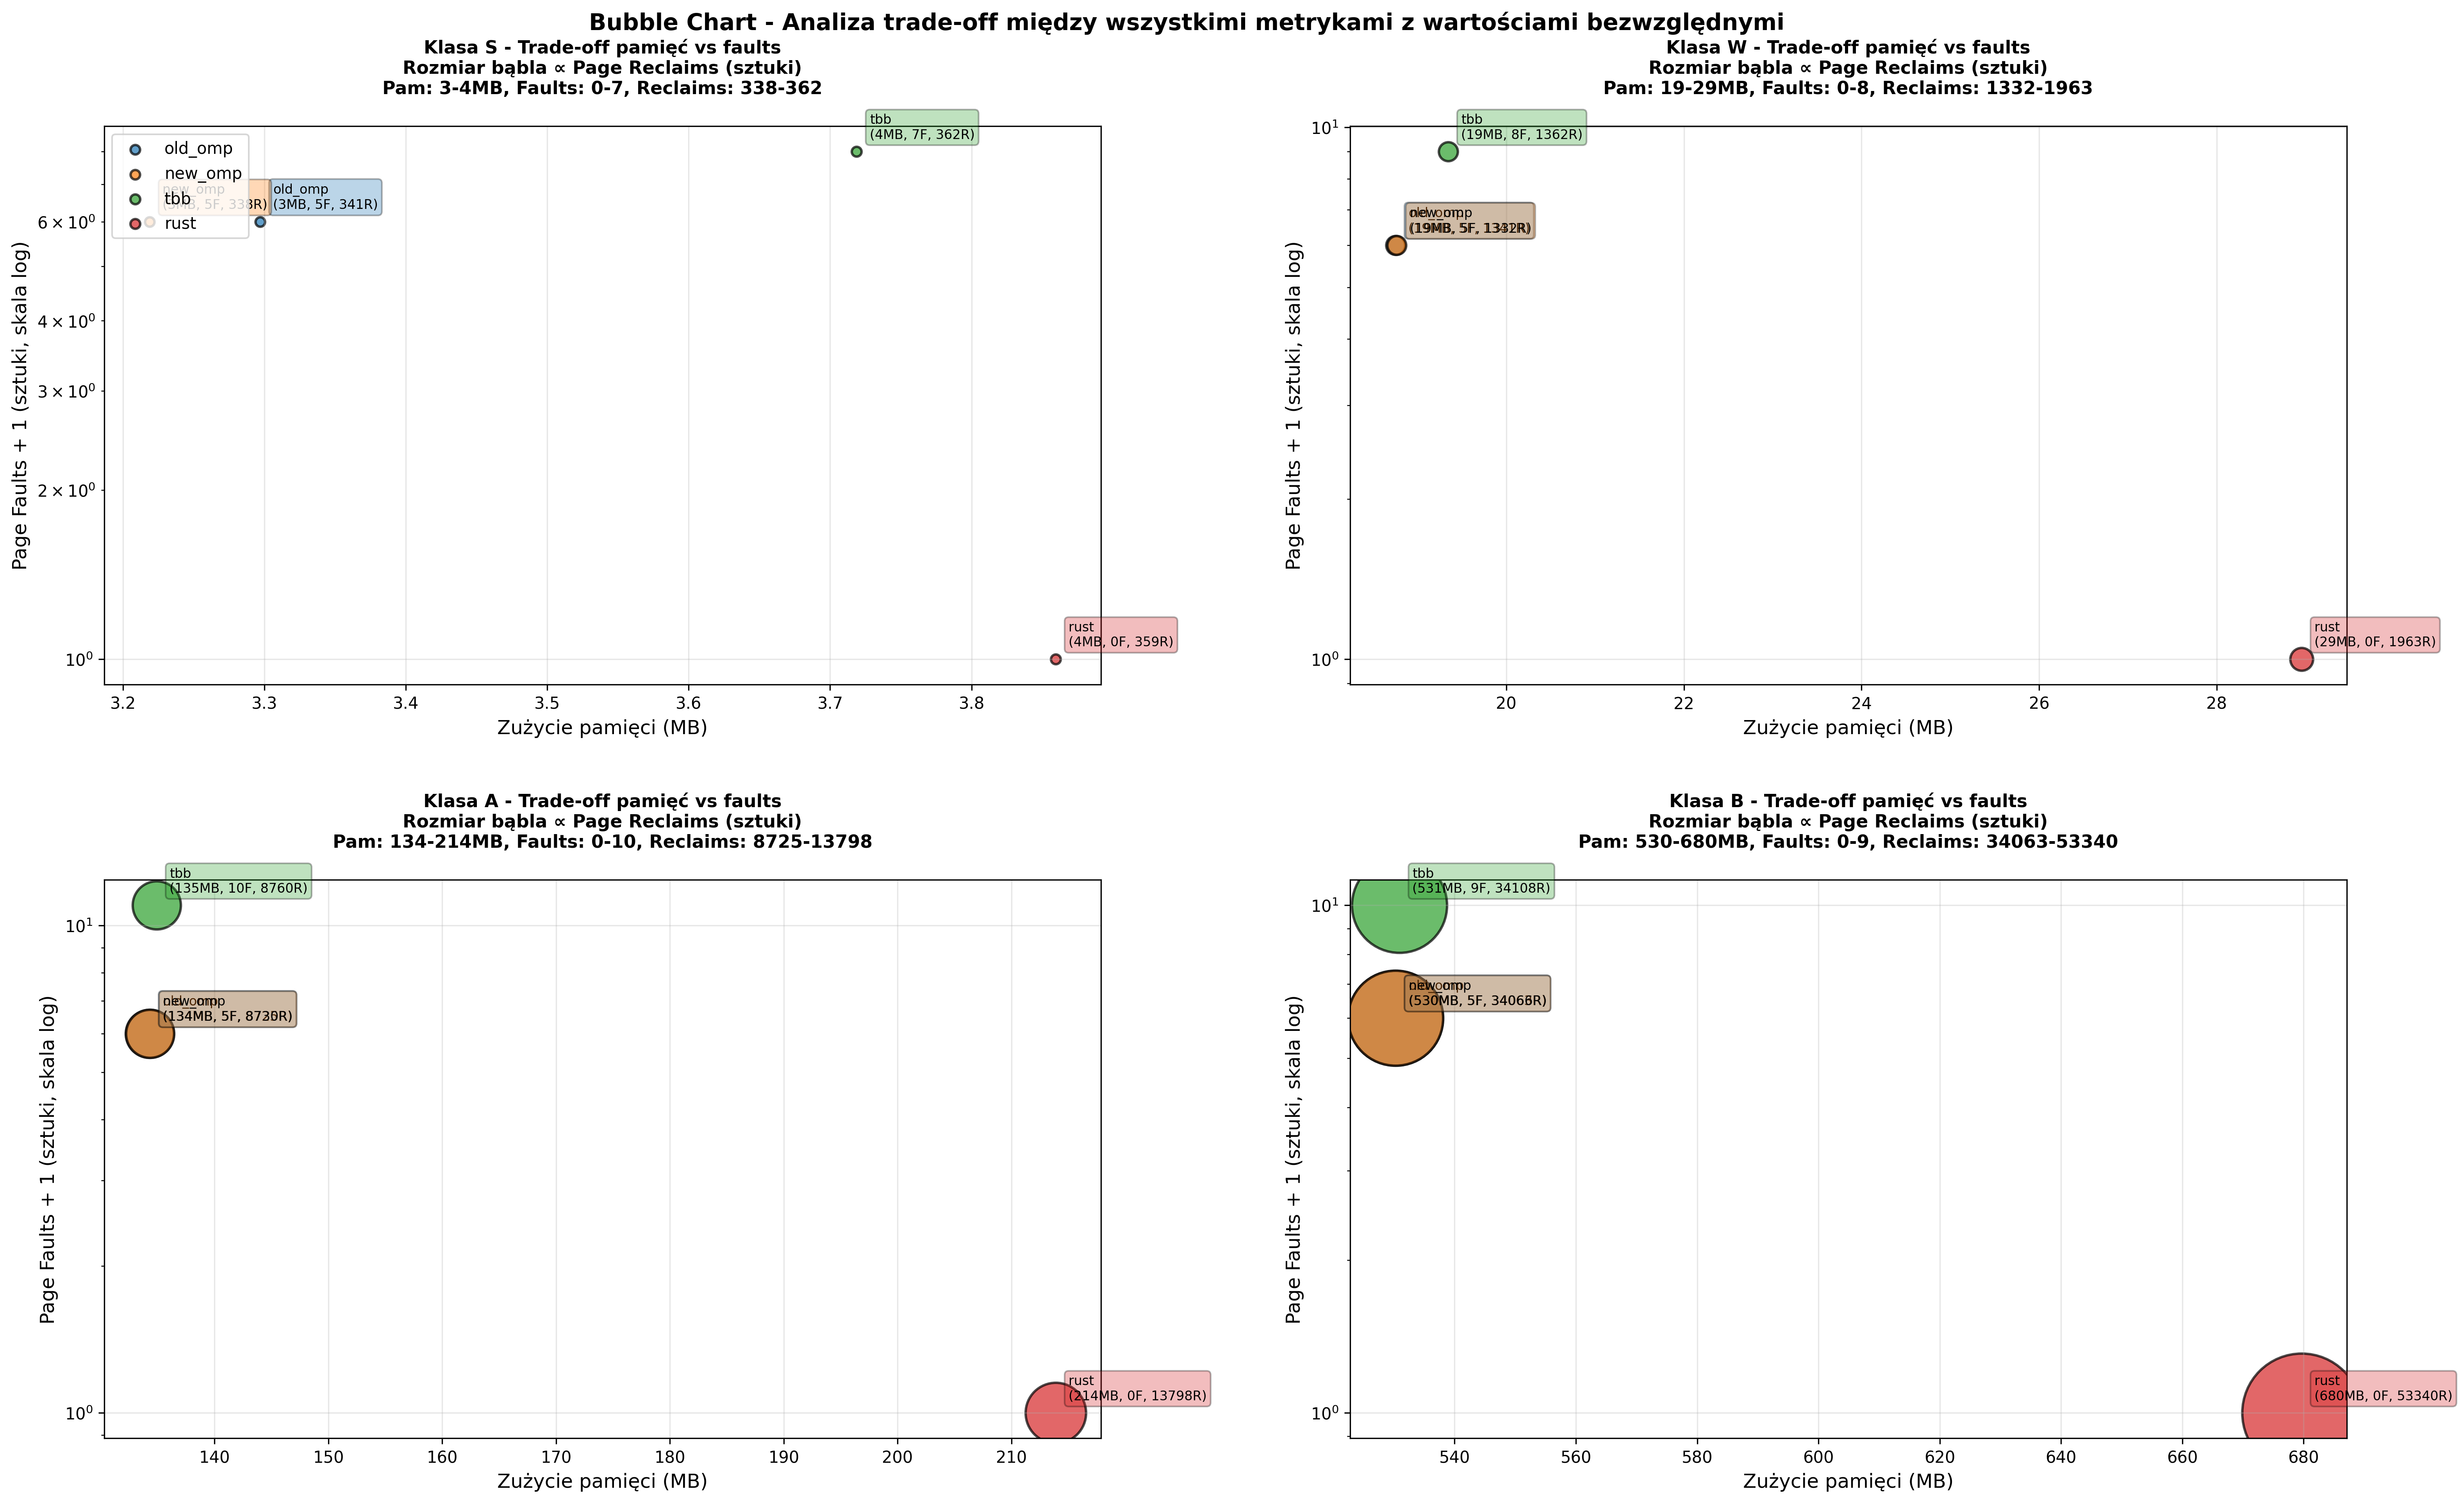
\includegraphics[width=0.9\textwidth]{analiza/images/parallel/is/arm/chart_06_bubble_chart.png}
    \caption{Kompromisy \eng{trade-off} pomiędzy zużyciem pamięci a błędami stron pamięci, z uwzględnieniem liczby odzyskanych stron jako trzeciej zmiennej reprezentowanej przez rozmiar bąbla}
    \label{is_kompromisy_pamiec_bledy}
\end{figure}
Na podstawie wykresu bąbelkowego - rysunek \ref{is_kompromisy_pamiec_bledy} można zauważyć:
\begin{itemize}
    \item \texttt{rust} w każdej klasie lokuje się w dolnym rejonie wykresu (niska liczba błędów) przy wysokim zużyciu pamięci oraz największych bąblach (najwięcej zwolnień stron).
    \item \texttt{tbb} regularnie generuje najwyższą liczbę błędów stron przy zbliżonym zużyciu pamięci jak \texttt{old\_omp} i \texttt{new\_omp}.
    \item \texttt{new\_omp} uzyskuje relatywnie zrównoważony kompromis - umiarkowane zużycie pamięci, średnia liczba błędów stron i średnia liczba odzyskanych stron.
\end{itemize}
\subsection{Wyniki profilowania wydajności - platforma x86\_64}
\begin{figure}[H]
    \centering
    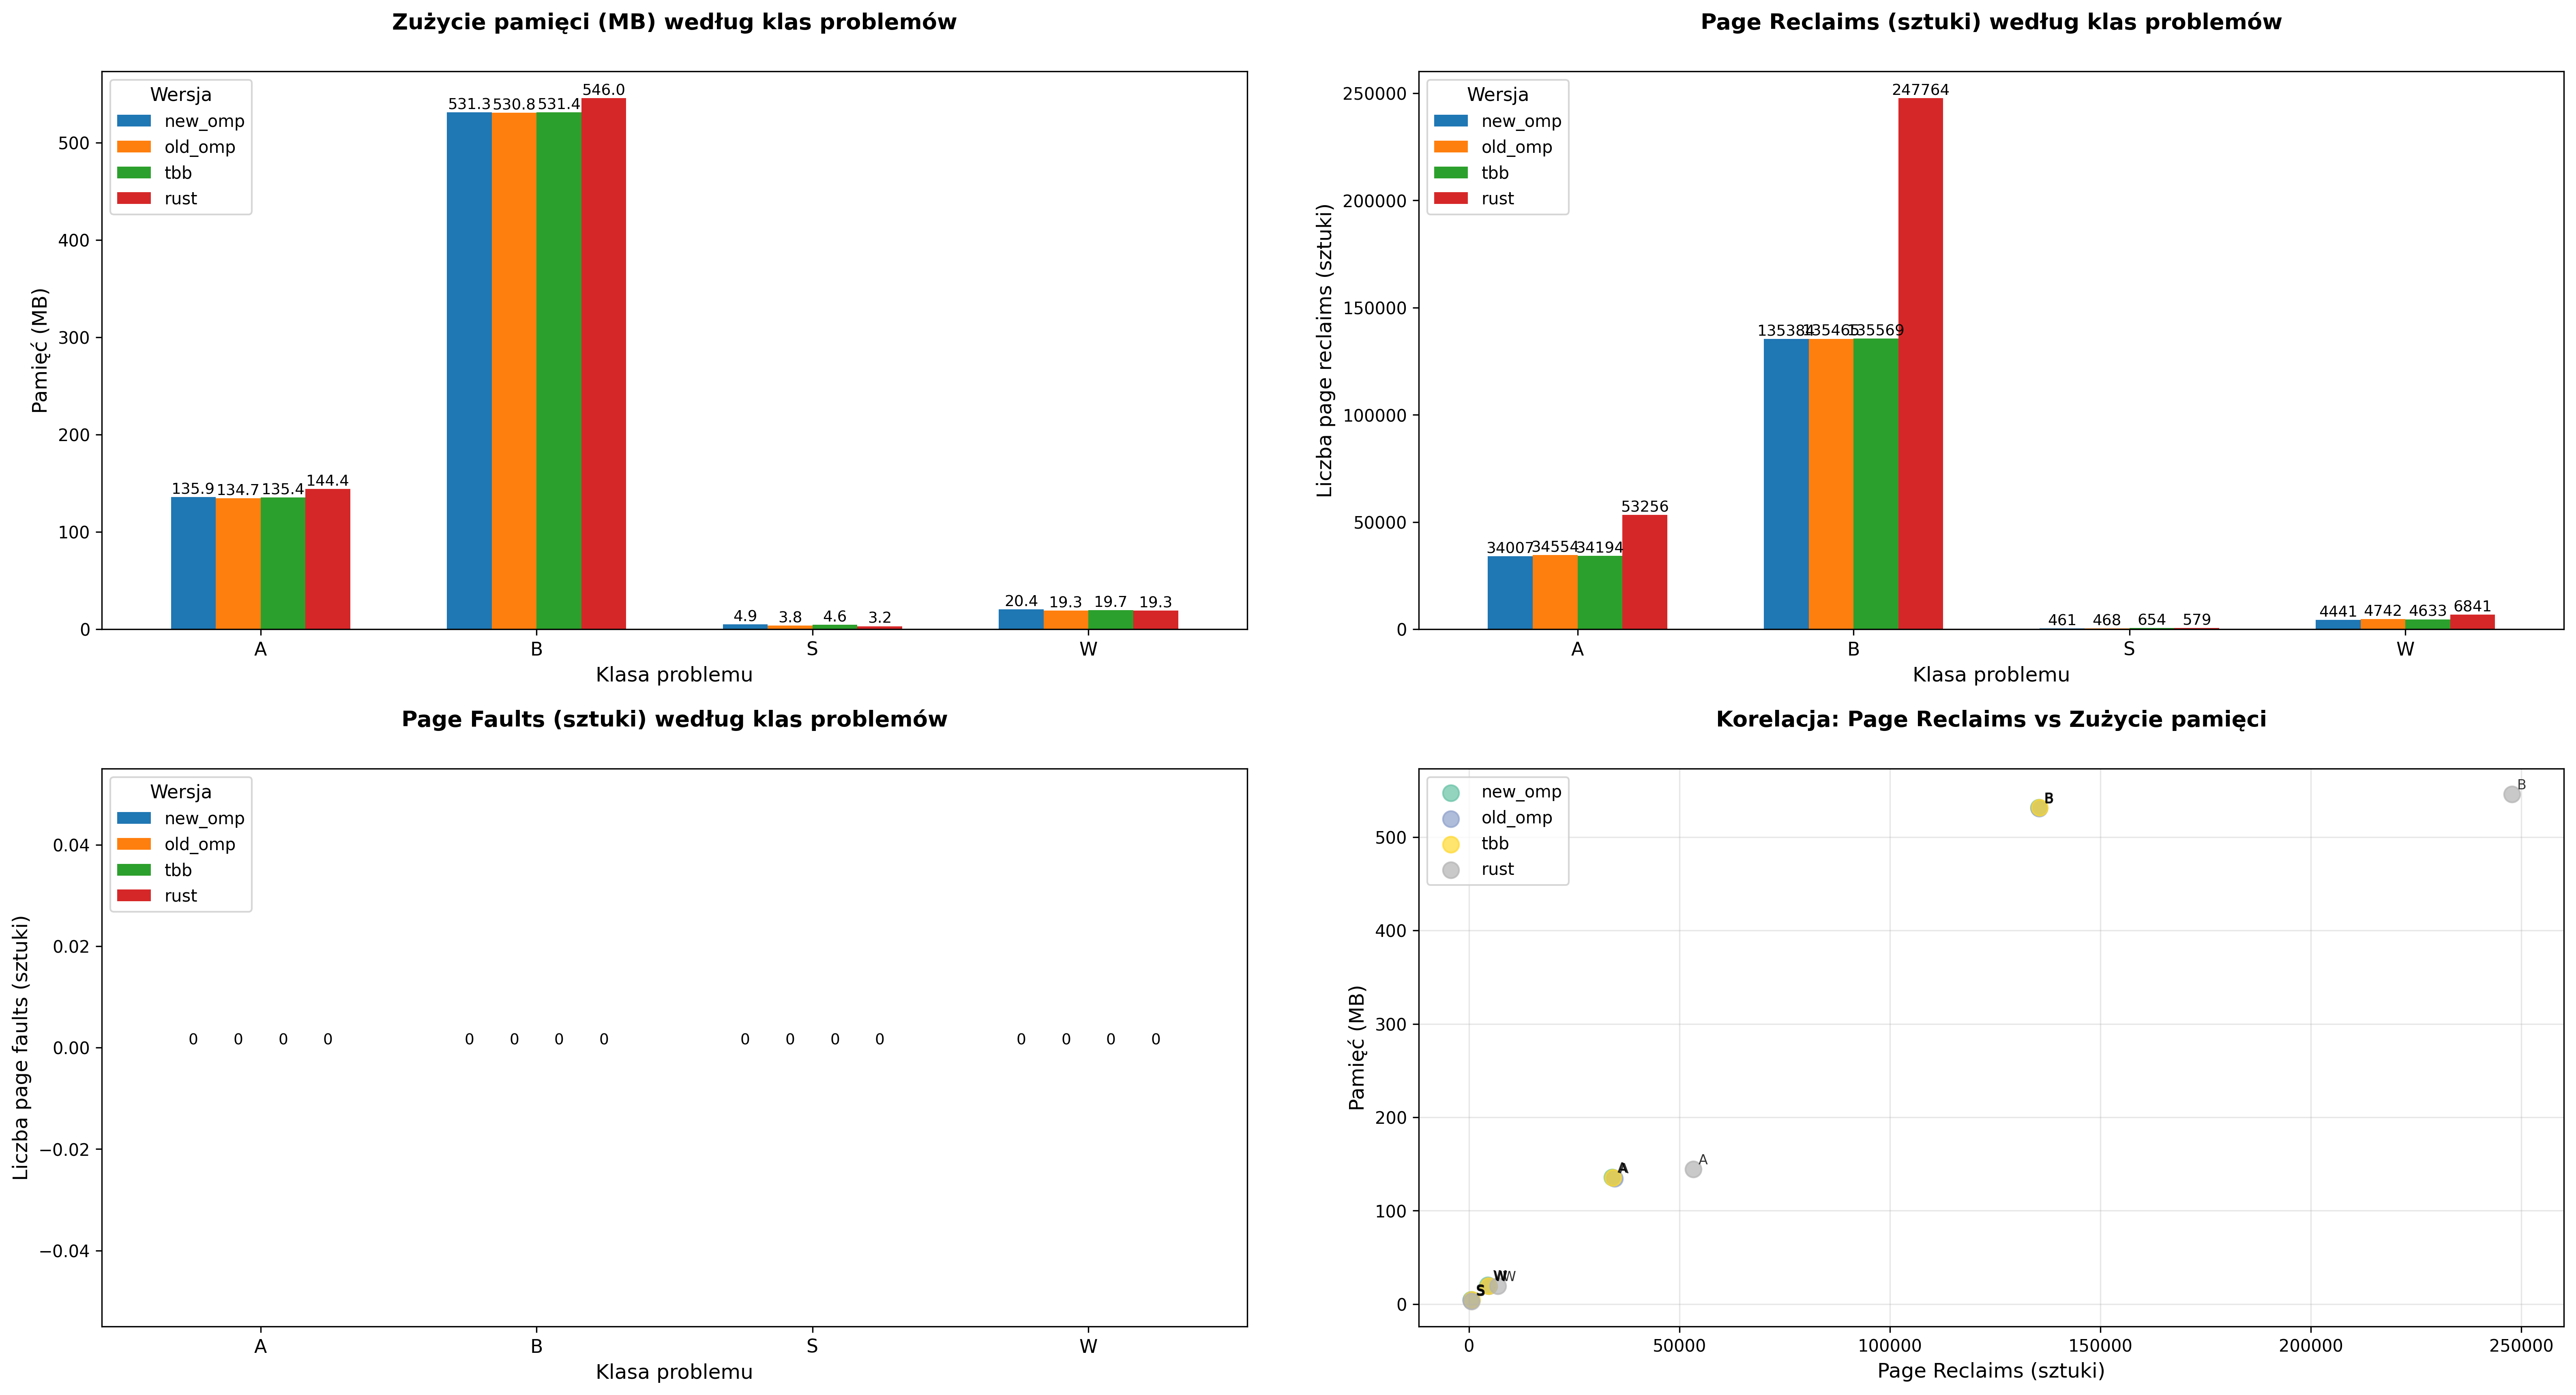
\includegraphics[width=0.9\textwidth]{analiza/images/parallel/is/x86/chart_01_memory_comparison.png}
    \caption{Profilowanie wydajności benchmarku IS dla klas S, W, A, B względem liczby użytych wątków}
    \label{is_porownanie_zuzycia_pamieci_x86}
\end{figure}

Analiza wykresów dotyczących zużycia pamięci - rysunek \ref{is_porownanie_zuzycia_pamieci_x86} ujawnia wyraźne różnice w~zapotrzebowaniu na zasoby w zależności od klasy problemu, przy jednoczesnym niewielkim zróżnicowaniu pomiędzy poszczególnymi implementacjami. Największe zużycie pamięci zaobserwowano dla klasy B, co jest bezpośrednio związane z największym rozmiarem sortowanych danych. W tej klasie implementacja w języku Rust wyróżnia się nieznacznie wyższym zużyciem pamięci (546 MB) w porównaniu do pozostałych (531-533 MB). Klasa A wykazuje umiarkowane zapotrzebowanie na pamięć, mieszczące się w zakresie 135-144 MB, z ponownym wskazaniem na implementację Rust jako najbardziej zasobożerną (144,4 MB). Dla klas S~i~W, ze względu na mniejszy rozmiar problemu, zużycie pamięci jest znacząco niższe i wynosi odpowiednio 3,2-4,9 MB oraz 19,3-20,4 MB. Co interesujące, w przypadku klasy S to właśnie implementacja Rust osiąga najniższe zużycie pamięci (3,2 MB).

Wykresy przedstawiające operacje pamięci wirtualnej (zwolnienia oraz błędy stron) - \ref{is_porownanie_zuzycia_pamieci_x86} dostarczają informacji o efektywności zarządzania pamięcią. Szczególnie widoczna jest wysoka liczba zwolnień stron pamięci w klasie B, gdzie implementacja Rust osiąga wartość 247 764, znacznie przewyższając inne implementacje oscylujące wokół 135 000-136 000. Podobna tendencja występuje w klasie A - Rust generuje 53 256 zwolnień stron, podczas gdy pozostałe implementacje utrzymują się na poziomie 34 000-35 000. W klasach S i W liczby te są proporcjonalnie mniejsze, co odpowiada ich ograniczonym wymaganiom pamięciowym.

Z kolei brak błędów stron we wszystkich implementacjach i klasach problemu jest jednoznacznym dowodem na skuteczne zarządzanie pamięcią przez system operacyjny. Brak konieczności odwołań do pamięci wymiany oznacza, że całość operacji wykonywana była w pamięci fizycznej, bez negatywnego wpływu na wydajność.

Wykres korelacyjny między liczbą zwolnień stron a zużyciem pamięci wskazuje na silną zależność między tymi dwiema metrykami. Dane tworzą wyraźne grupy odpowiadające klasom problemu - od klasy B z najwyższym zużyciem pamięci, po klasę S z najniższym. W ramach każdej grupy implementacja Rust wykazuje tendencję do generowania większej liczby reklamacji stron przy podobnym zużyciu pamięci, co może świadczyć o jej specyficznym podejściu do alokacji i zwalniania pamięci - bardziej intensywnym, lecz potencjalnie korzystnym dla innych aspektów wydajności.
\begin{figure}[H]
    \centering
    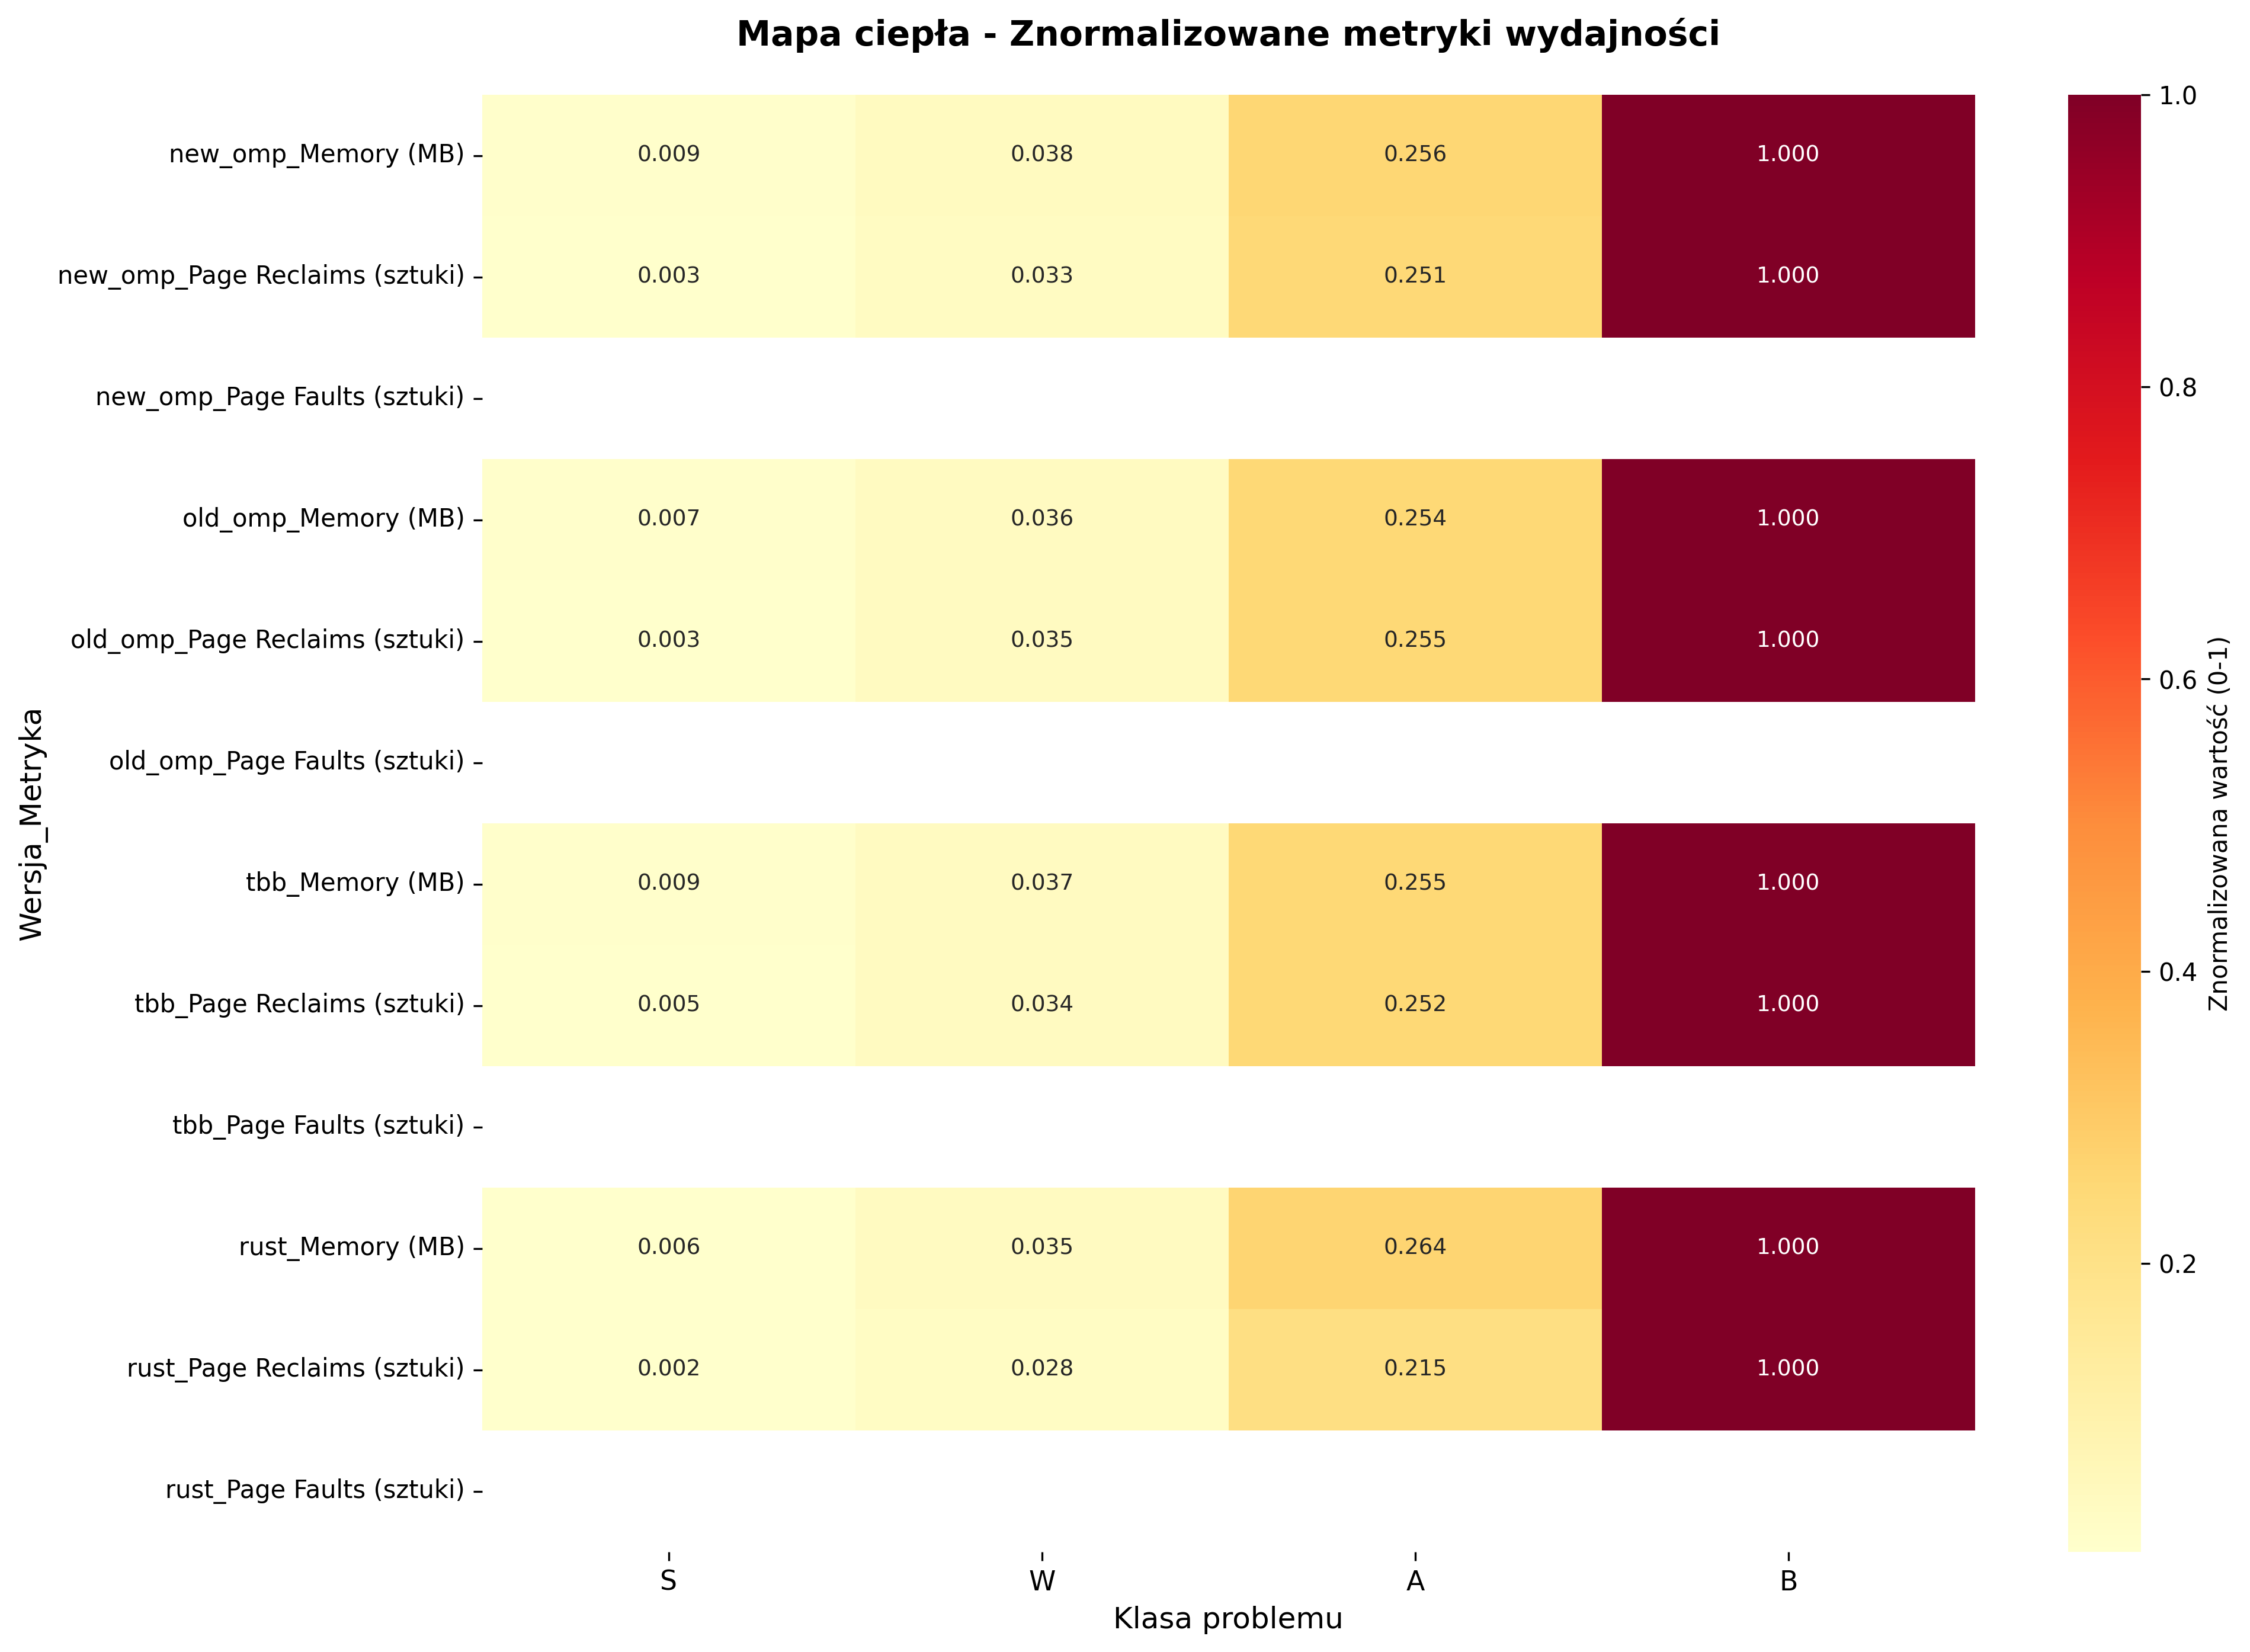
\includegraphics[width=0.9\textwidth]{analiza/images/parallel/is/x86/chart_03_heatmap.png}
    \caption{Znormalizowana mapa ciepła metryk wydajności}
    \label{is_heatmap_wydajnosci_x86}
\end{figure}
Znormalizowana mapa ciepła metryk wydajności - rysunek \ref{is_heatmap_wydajnosci_x86} potwierdza powyższe obserwacje, ukazując proporcjonalne różnice między klasami problemu i implementacjami. Wzorzec ten nie tylko podkreśla wpływ rozmiaru problemu na charakterystyki pamięciowe, ale również zwraca uwagę na unikalne właściwości implementacji Rust, której strategia zarządzania pamięcią istotnie różni się od pozostałych rozwiązań.

\subsection{Porównanie pomiędzy platformami}
\begin{figure}[H]
    \centering
    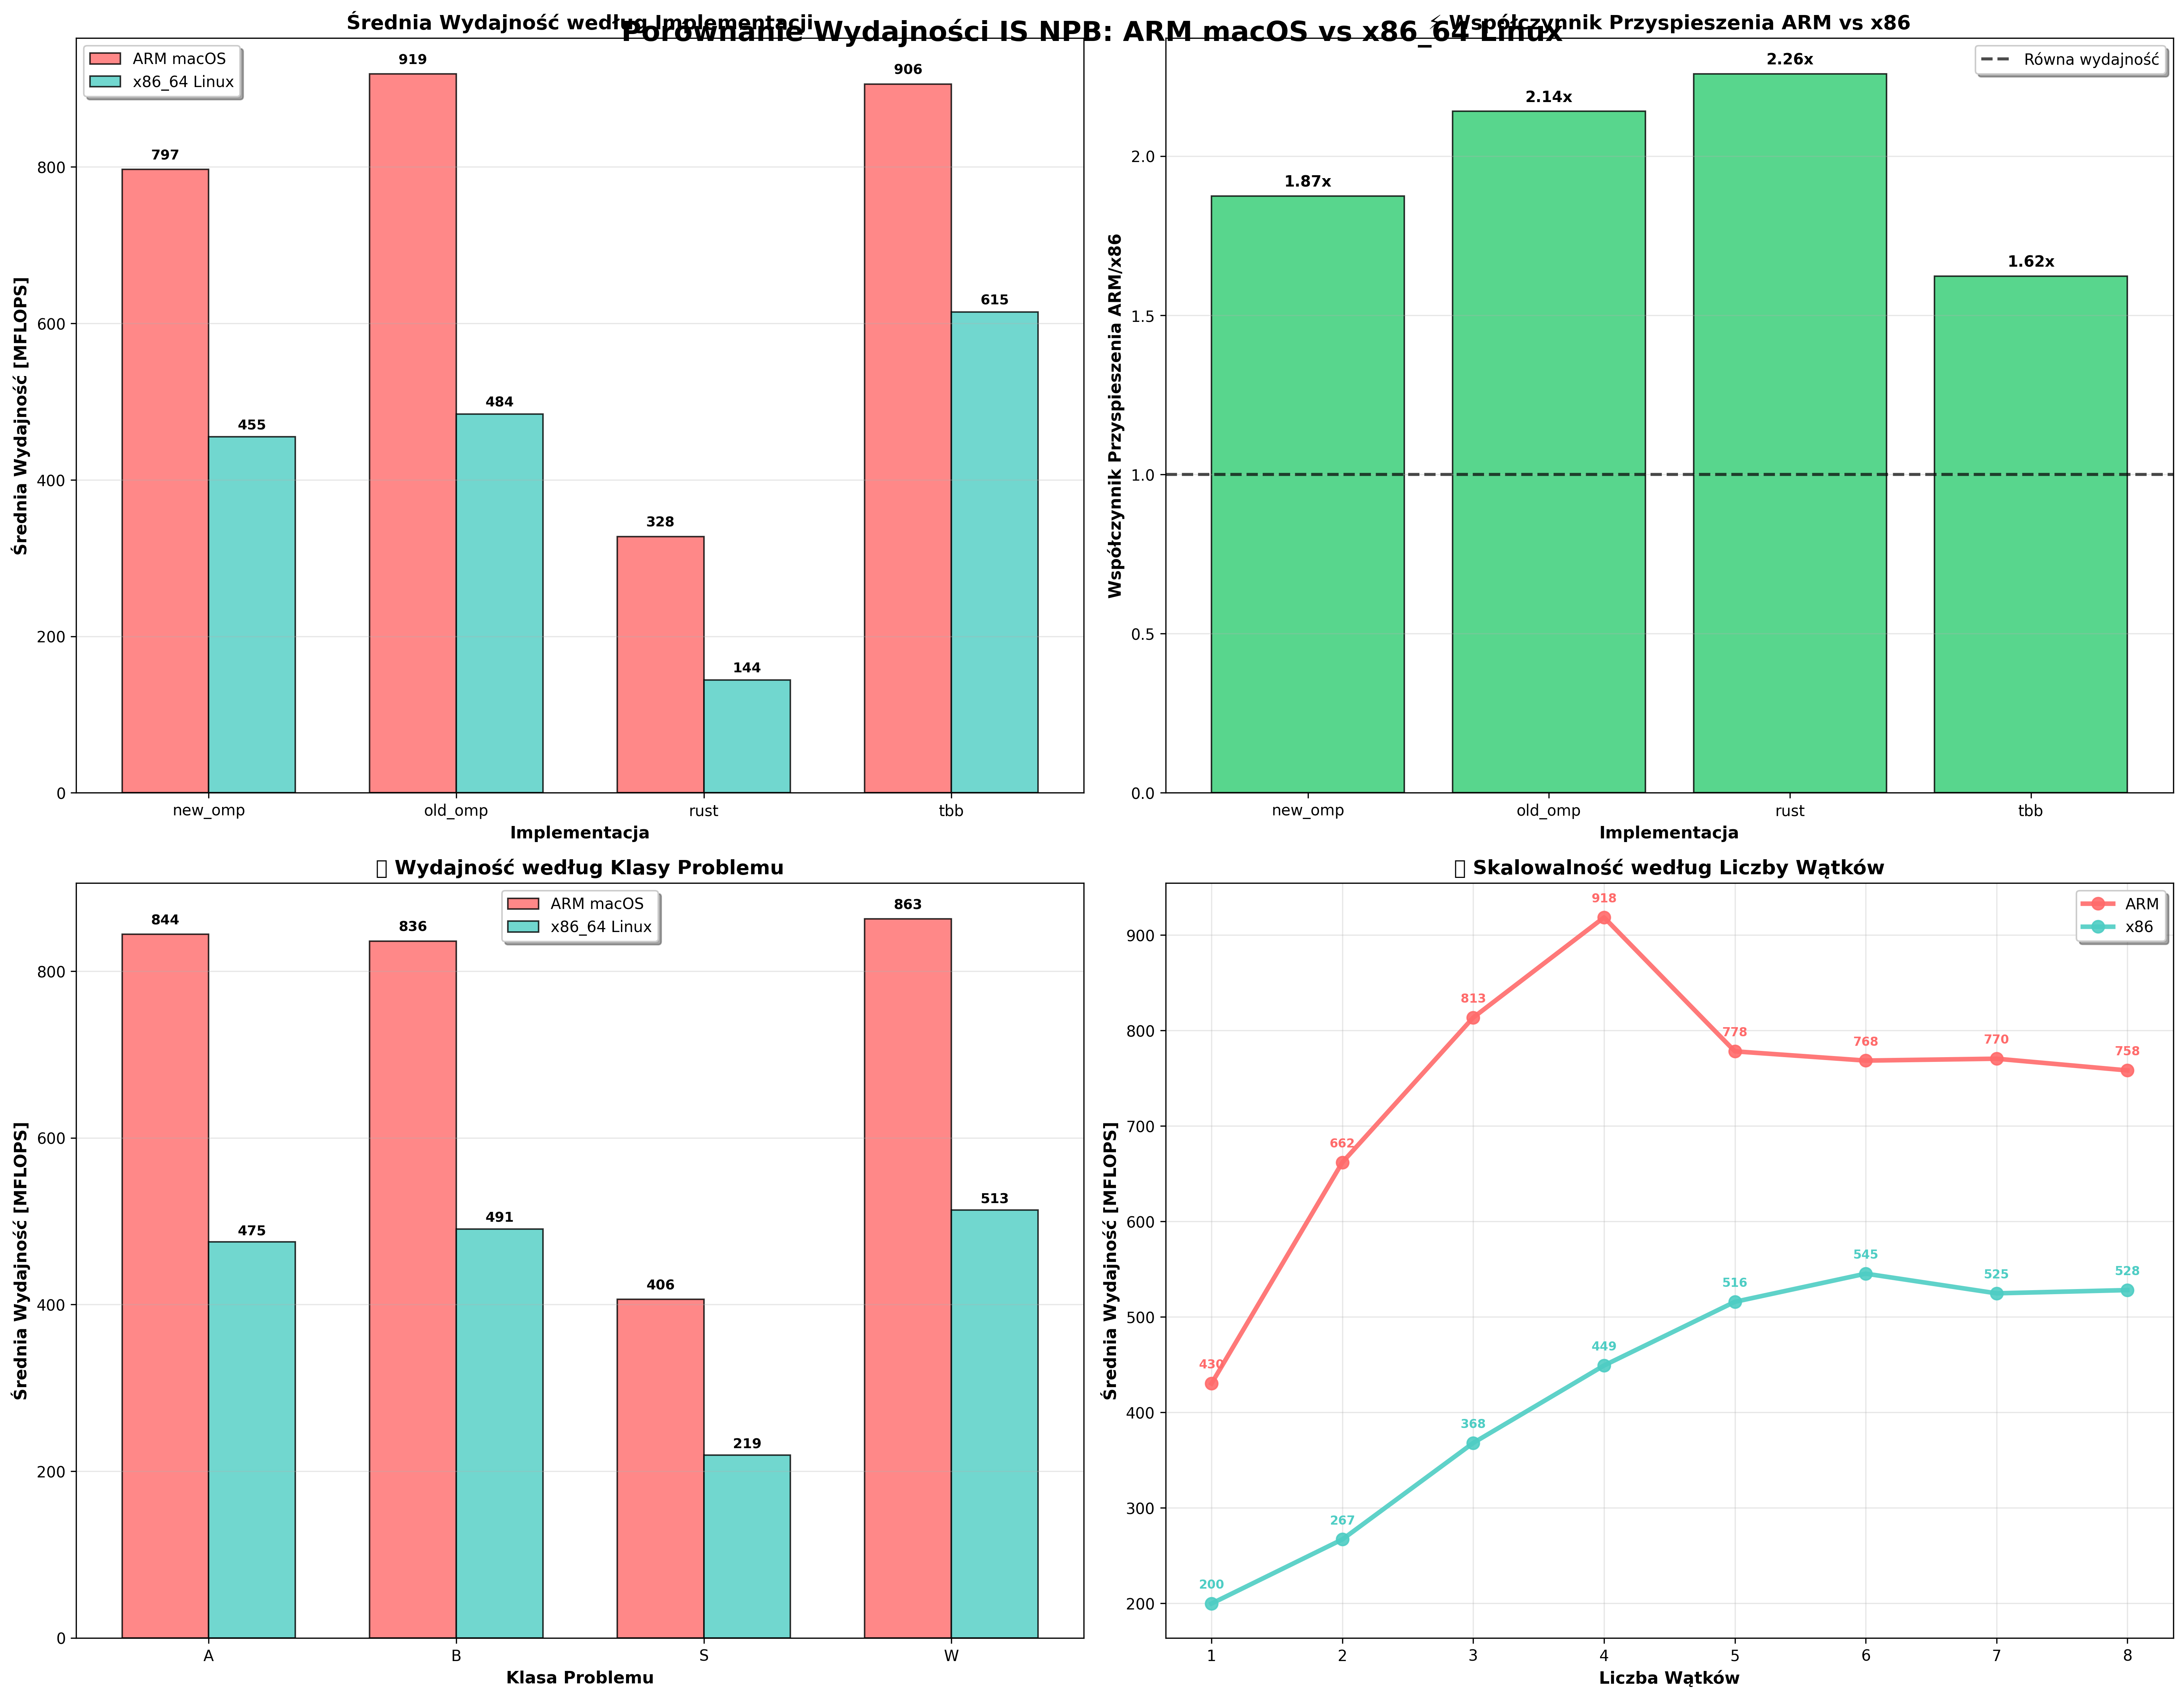
\includegraphics[width=0.9\textwidth]{analiza/images/parallel/is/compare/is_porownanie_platform_arm_vs_x86.png}
    \caption{Porównanie średniej wydajności benchmarku IS dla platform ARM64 i x86\_64}
    \label{is_porownanie_wydajnosci_platformy}
\end{figure}
\subsubsection{Analiza średniej wydajności według implementacji}
Górny lewy wykres drugiego zestawu - rysunek \ref{is_porownanie_wydajnosci_platformy} prezentuje średnią wydajność dla różnych implementacji algorytmów. We wszystkich badanych przypadkach (new\_cmp, old\_cmp, \texttt{rust}, \texttt{tbb}) architektura ARM macOS osiąga znacząco wyższe wartości MFLOPS niż architektura x86\_64 Linux. Szczególnie wyraźna przewaga ARM występuje w implementacjach old\_cmp (916 a 484 MFLOPS) oraz \texttt{tbb} (906 a 615 MFLOPS).

Współczynnik przyspieszenia widoczny w prawym górnym wykresie - \ref{is_porownanie_wydajnosci_platformy} potwierdza tę przewagę, wskazując że implementacja w języku Rust osiąga najwyższy współczynnik przyspieszenia (2,34x), a tuż za nią plasuje się implementacja \texttt{tbb} (2,26x). Wszystkie badane implementacje wykazują wartości współczynnika przyspieszenia powyżej 1,0, co potwierdza systematyczną przewagę wydajnościową platformy ARM.

\subsubsection{Analiza wydajności według klasy problemu i skalowalności}
Lewy dolny wykres drugiego zestawu - rysunek \ref{is_porownanie_wydajnosci_platformy} ilustruje, że przewaga wydajnościowa ARM macOS utrzymuje się konsekwentnie we wszystkich klasach problemów (A, B, C oraz W). Warto zauważyć, że różnica wydajnościowa jest proporcjonalna do złożoności problemu.

Analiza skalowalności według liczby wątków (prawy dolny wykres) pokazuje, że obie platformy wykazują wzrost wydajności wraz ze zwiększaniem liczby wątków do około 4-5, po czym następuje stabilizacja lub lekki spadek. ARM macOS konsekwentnie utrzymuje wyższą bezwzględną wydajność, przy czym najwyższa wartość przypada na 4 wątki (913 MFLOPS dla ARM a 518 MFLOPS dla x86\_64).

\begin{figure}[!h]
    \centering
    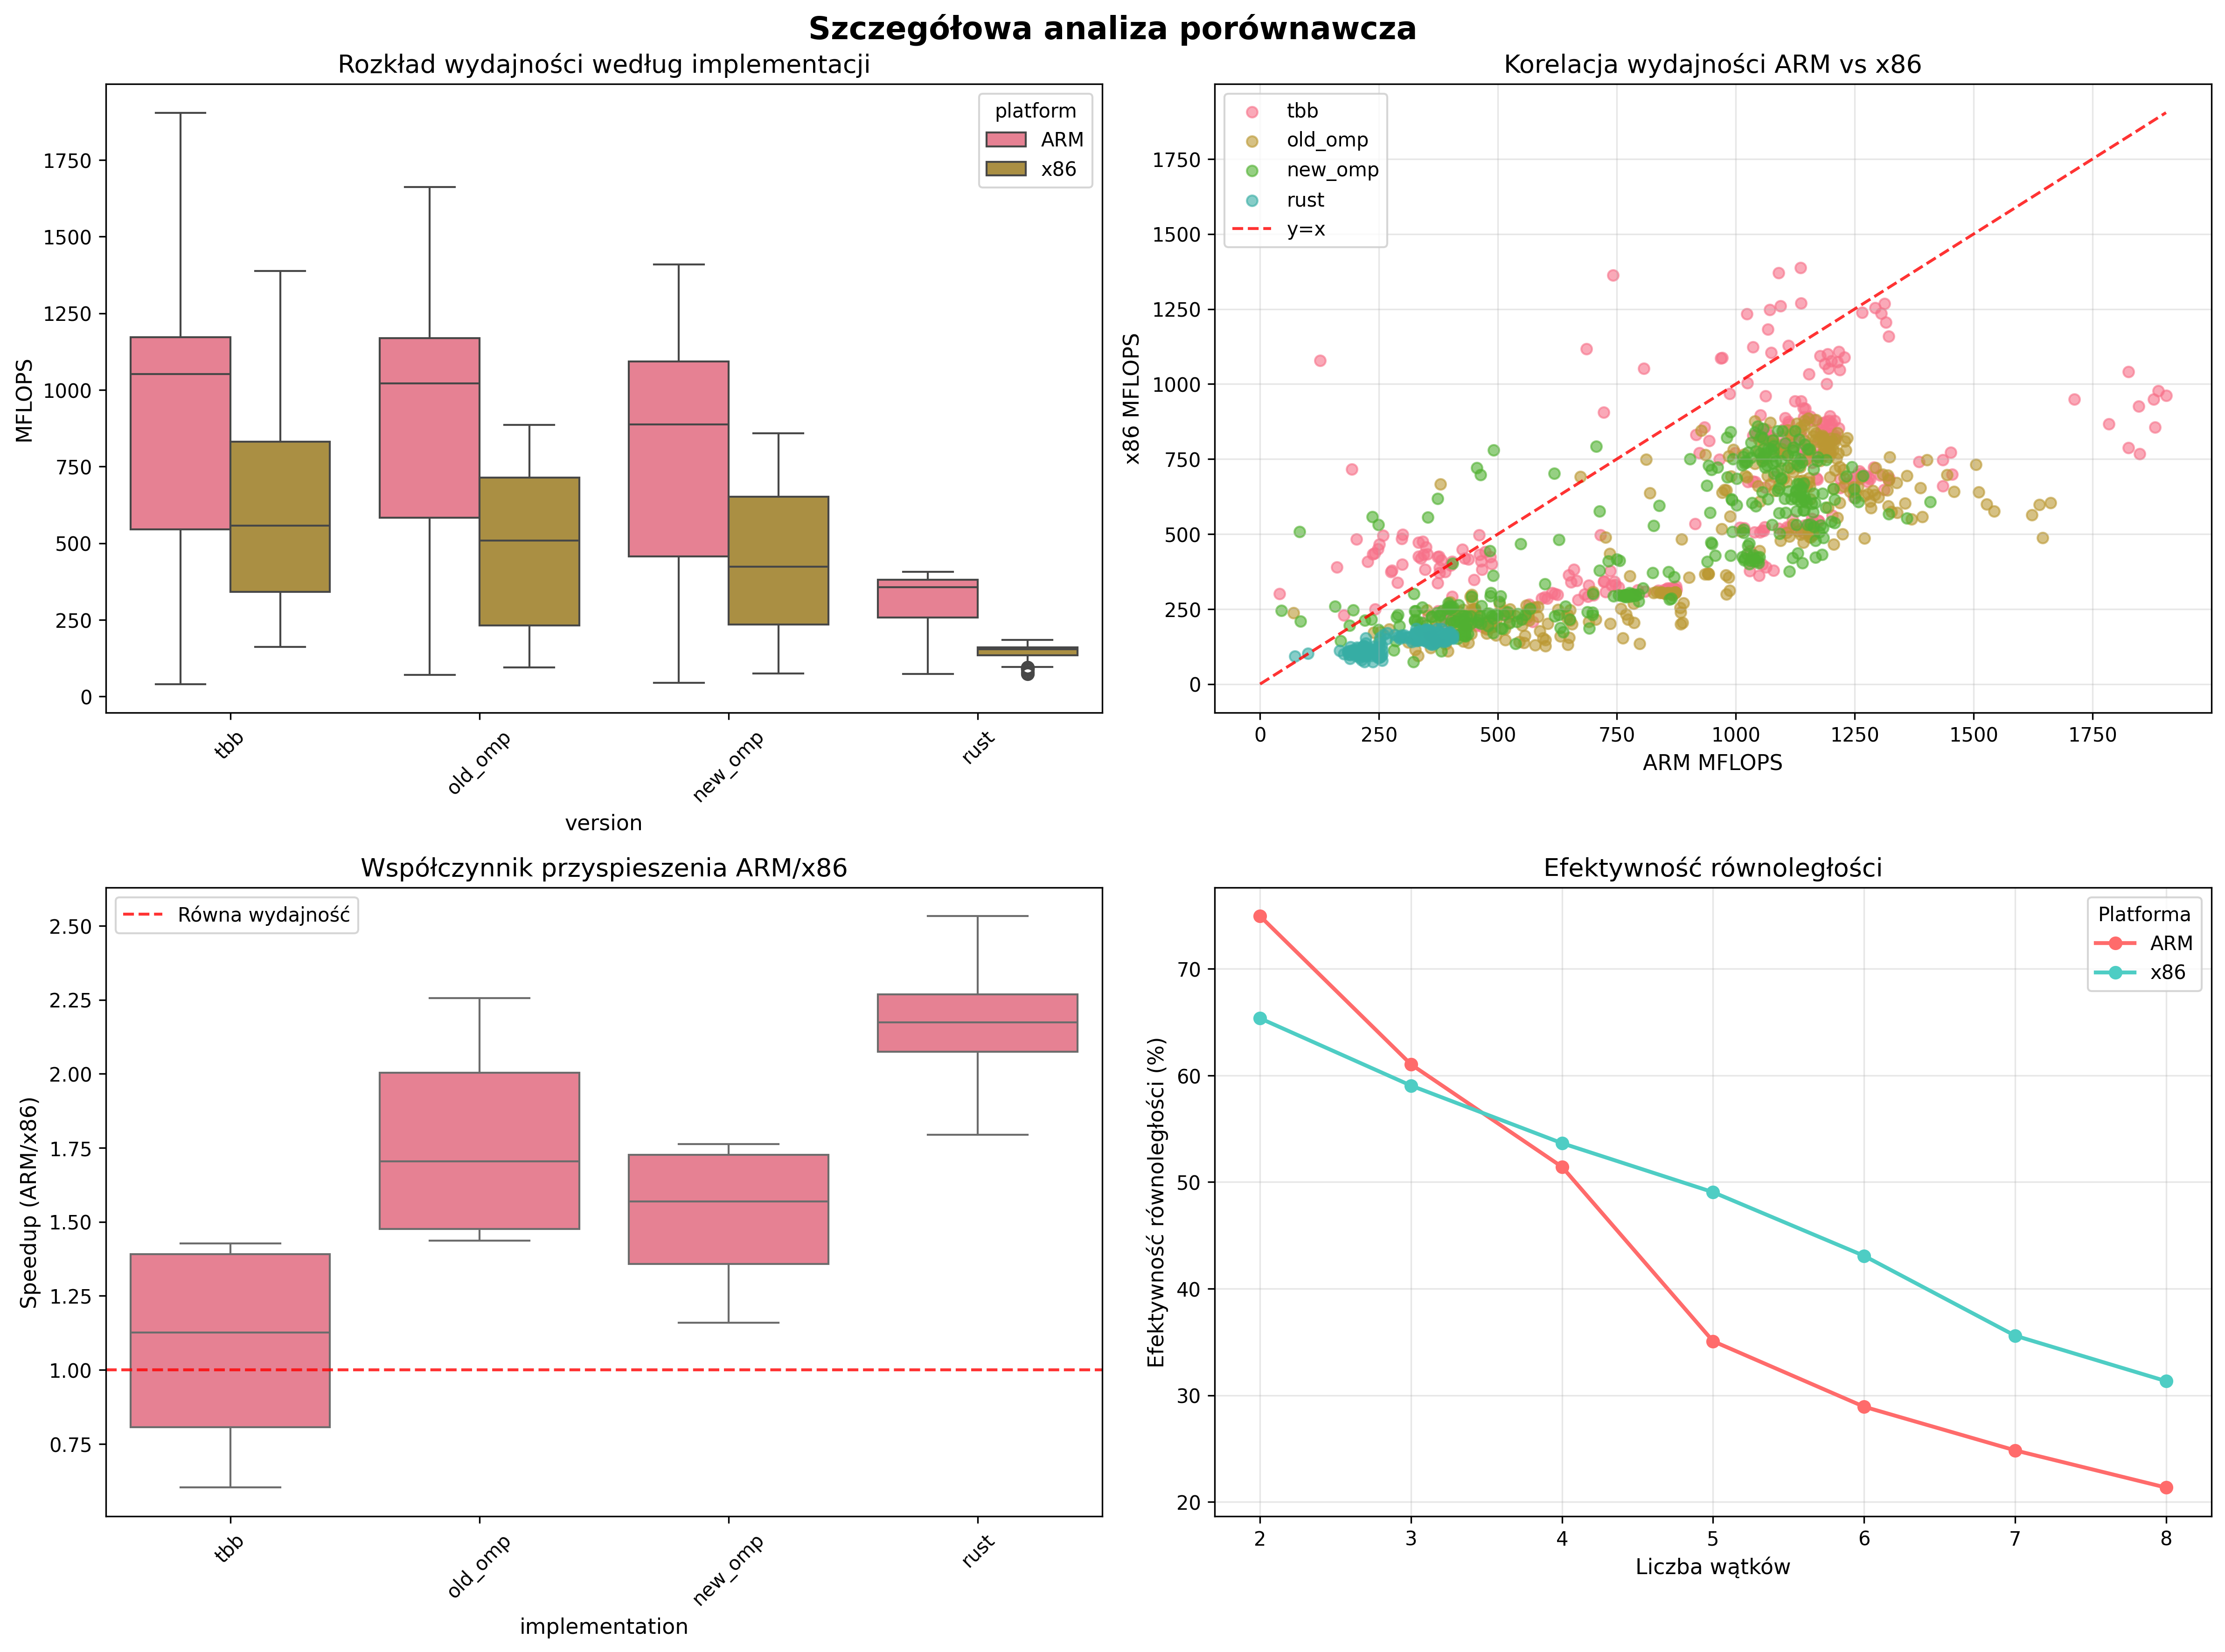
\includegraphics[width=0.9\textwidth]{analiza/images/parallel/is/compare/is_szczegolowa_analiza_wydajnosci.png}
    \caption{Szczegółowa analiza wydajności benchmarku IS dla platform ARM64 i x86\_64}
    \label{is_szczegolowa_analiza_wydajnosci}
\end{figure}
Wykresy pudełkowe - rysunek \ref{is_szczegolowa_analiza_wydajnosci} potwierdzają, że mediana wydajności dla platformy ARM jest systematycznie wyższa niż dla x86\_64 we wszystkich implementacjach. Jednocześnie platforma ARM charakteryzuje się większym rozrzutem wyników, co sugeruje większą zmienność wydajności.

Wykres korelacji wydajności ARM a x86 z kodowaniem kolorystycznym różnych implementacji dodatkowo potwierdza, że większość punktów pomiarowych znajduje się powyżej linii równej wydajności, przy czym różne implementacje grupują się w odmiennych obszarach wydajnościowych.

Analiza współczynnika przyspieszenia wskazuje, że implementacja Rust osiąga najwyższy medianowy współczynnik przyspieszenia (około 2,2x), natomiast implementacja \texttt{tbb} wykazuje największą zmienność, z niektórymi przypadkami osiągającymi wartości poniżej 1,0.

Ostatni wykres przedstawia efektywność równoległości w zależności od liczby wątków. Architektura ARM rozpoczyna z wyższą efektywnością przy małej liczbie wątków, jednak doświadcza szybszego spadku efektywności wraz ze wzrostem liczby wątków. Przy 8 wątkach obie platformy osiągają efektywność około 30\%, przy czym x86\_64 wypada nieznacznie lepiej, co wskazuje na lepsze zachowanie skalowalności przy wyższej liczbie wątków.
\begin{figure}[H]
    \centering
    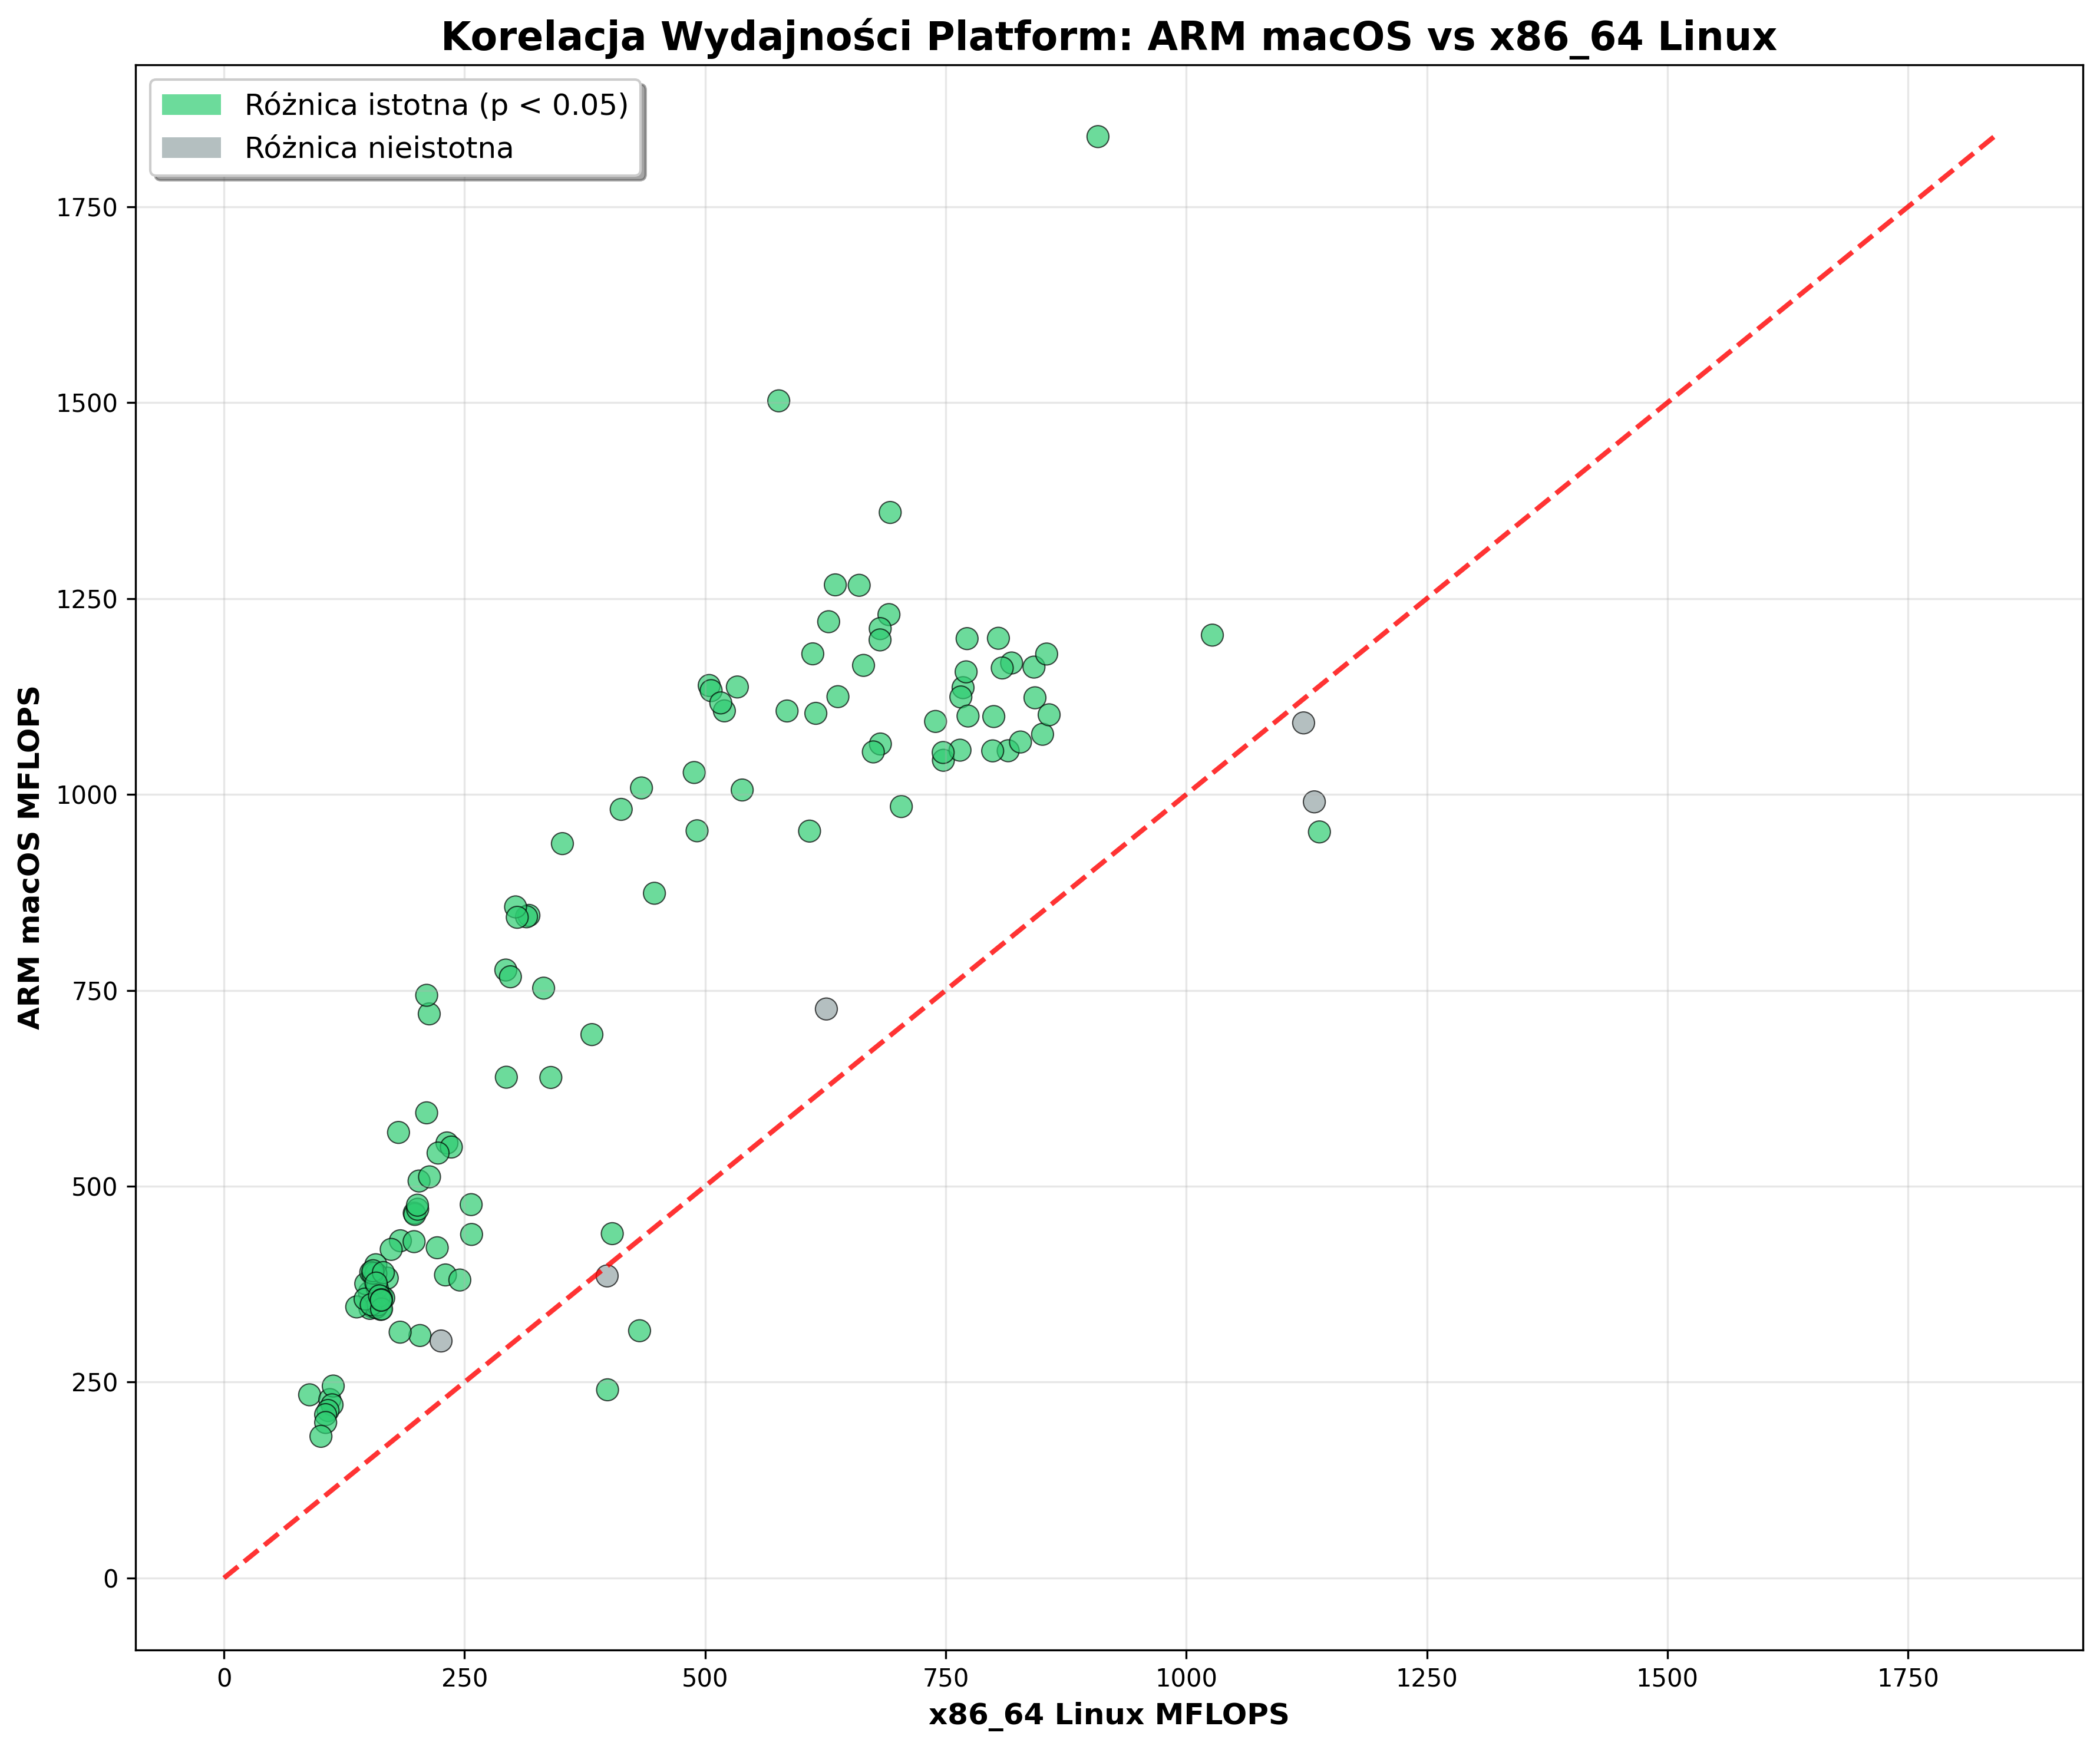
\includegraphics[width=0.9\textwidth]{analiza/images/parallel/is/compare/is_analiza_istotnosci_statystycznej.png}
    \caption{Analiza istotności statystycznej benchmarku IS dla platform ARM64 i x86\_64}
    \label{is_analiza_istotnosci_statystycznej}
\end{figure}
Przedstawiony na wykresie rozkład punktów obrazuje korelację między wydajnością (mierzoną w MFLOPS - miliony operacji zmiennoprzecinkowych na sekundę) - rysunek \ref{is_szczegolowa_analiza_wydajnosci} na platformie ARM macOS względem x86\_64 Linux. Punkty oznaczone kolorem zielonym wskazują na statystycznie istotne różnice (p < 0,05), natomiast punkty szare reprezentują różnice nieistotne statystycznie. Czerwona przerywana linia reprezentuje teoretyczną równą wydajność obu platform (y=x). Zdecydowana większość punktów znajduje się powyżej tej linii, co jednoznacznie wskazuje na przewagę wydajnościową architektury ARM macOS nad x86\_64 Linux w badanych przypadkach.

